% Options for packages loaded elsewhere
% Options for packages loaded elsewhere
\PassOptionsToPackage{unicode}{hyperref}
\PassOptionsToPackage{hyphens}{url}
\PassOptionsToPackage{dvipsnames,svgnames,x11names}{xcolor}
%
\documentclass[
  letterpaper,
  DIV=11,
  numbers=noendperiod]{scrartcl}
\usepackage{xcolor}
\usepackage{amsmath,amssymb}
\setcounter{secnumdepth}{5}
\usepackage{iftex}
\ifPDFTeX
  \usepackage[T1]{fontenc}
  \usepackage[utf8]{inputenc}
  \usepackage{textcomp} % provide euro and other symbols
\else % if luatex or xetex
  \usepackage{unicode-math} % this also loads fontspec
  \defaultfontfeatures{Scale=MatchLowercase}
  \defaultfontfeatures[\rmfamily]{Ligatures=TeX,Scale=1}
\fi
\usepackage{lmodern}
\ifPDFTeX\else
  % xetex/luatex font selection
\fi
% Use upquote if available, for straight quotes in verbatim environments
\IfFileExists{upquote.sty}{\usepackage{upquote}}{}
\IfFileExists{microtype.sty}{% use microtype if available
  \usepackage[]{microtype}
  \UseMicrotypeSet[protrusion]{basicmath} % disable protrusion for tt fonts
}{}
\makeatletter
\@ifundefined{KOMAClassName}{% if non-KOMA class
  \IfFileExists{parskip.sty}{%
    \usepackage{parskip}
  }{% else
    \setlength{\parindent}{0pt}
    \setlength{\parskip}{6pt plus 2pt minus 1pt}}
}{% if KOMA class
  \KOMAoptions{parskip=half}}
\makeatother
% Make \paragraph and \subparagraph free-standing
\makeatletter
\ifx\paragraph\undefined\else
  \let\oldparagraph\paragraph
  \renewcommand{\paragraph}{
    \@ifstar
      \xxxParagraphStar
      \xxxParagraphNoStar
  }
  \newcommand{\xxxParagraphStar}[1]{\oldparagraph*{#1}\mbox{}}
  \newcommand{\xxxParagraphNoStar}[1]{\oldparagraph{#1}\mbox{}}
\fi
\ifx\subparagraph\undefined\else
  \let\oldsubparagraph\subparagraph
  \renewcommand{\subparagraph}{
    \@ifstar
      \xxxSubParagraphStar
      \xxxSubParagraphNoStar
  }
  \newcommand{\xxxSubParagraphStar}[1]{\oldsubparagraph*{#1}\mbox{}}
  \newcommand{\xxxSubParagraphNoStar}[1]{\oldsubparagraph{#1}\mbox{}}
\fi
\makeatother


\usepackage{longtable,booktabs,array}
\newcounter{none} % for unnumbered tables
\usepackage{calc} % for calculating minipage widths
% Correct order of tables after \paragraph or \subparagraph
\usepackage{etoolbox}
\makeatletter
\patchcmd\longtable{\par}{\if@noskipsec\mbox{}\fi\par}{}{}
\makeatother
% Allow footnotes in longtable head/foot
\IfFileExists{footnotehyper.sty}{\usepackage{footnotehyper}}{\usepackage{footnote}}
\makesavenoteenv{longtable}
\usepackage{graphicx}
\makeatletter
\newsavebox\pandoc@box
\newcommand*\pandocbounded[1]{% scales image to fit in text height/width
  \sbox\pandoc@box{#1}%
  \Gscale@div\@tempa{\textheight}{\dimexpr\ht\pandoc@box+\dp\pandoc@box\relax}%
  \Gscale@div\@tempb{\linewidth}{\wd\pandoc@box}%
  \ifdim\@tempb\p@<\@tempa\p@\let\@tempa\@tempb\fi% select the smaller of both
  \ifdim\@tempa\p@<\p@\scalebox{\@tempa}{\usebox\pandoc@box}%
  \else\usebox{\pandoc@box}%
  \fi%
}
% Set default figure placement to htbp
\def\fps@figure{htbp}
\makeatother


% definitions for citeproc citations
\NewDocumentCommand\citeproctext{}{}
\NewDocumentCommand\citeproc{mm}{%
  \begingroup\def\citeproctext{#2}\cite{#1}\endgroup}
\makeatletter
 % allow citations to break across lines
 \let\@cite@ofmt\@firstofone
 % avoid brackets around text for \cite:
 \def\@biblabel#1{}
 \def\@cite#1#2{{#1\if@tempswa , #2\fi}}
\makeatother
\newlength{\cslhangindent}
\setlength{\cslhangindent}{1.5em}
\newlength{\csllabelwidth}
\setlength{\csllabelwidth}{3em}
\newenvironment{CSLReferences}[2] % #1 hanging-indent, #2 entry-spacing
 {\begin{list}{}{%
  \setlength{\itemindent}{0pt}
  \setlength{\leftmargin}{0pt}
  \setlength{\parsep}{0pt}
  % turn on hanging indent if param 1 is 1
  \ifodd #1
   \setlength{\leftmargin}{\cslhangindent}
   \setlength{\itemindent}{-1\cslhangindent}
  \fi
  % set entry spacing
  \setlength{\itemsep}{#2\baselineskip}}}
 {\end{list}}
\usepackage{calc}
\newcommand{\CSLBlock}[1]{\hfill\break\parbox[t]{\linewidth}{\strut\ignorespaces#1\strut}}
\newcommand{\CSLLeftMargin}[1]{\parbox[t]{\csllabelwidth}{\strut#1\strut}}
\newcommand{\CSLRightInline}[1]{\parbox[t]{\linewidth - \csllabelwidth}{\strut#1\strut}}
\newcommand{\CSLIndent}[1]{\hspace{\cslhangindent}#1}



\setlength{\emergencystretch}{3em} % prevent overfull lines

\providecommand{\tightlist}{%
  \setlength{\itemsep}{0pt}\setlength{\parskip}{0pt}}



 


% load packages
\usepackage{geometry}
\usepackage{xcolor}
\usepackage{eso-pic}
\usepackage{fancyhdr}
\usepackage{sectsty}
\usepackage{fontspec}
\usepackage{titlesec}
\usepackage{graphicx}
\usepackage{tikz}
\usepackage{amsmath}
\usepackage{amssymb}
\usepackage{unicode-math}
  
%% Set page size with a wider right margin
\geometry{a4paper, total={170mm,257mm}, left=25mm, top=20mm, bottom=20mm, right=25mm}

%% Let's define some colours
\definecolor{light}{HTML}{F4F6F8}   % code-block background (_extension.yml: code-block-bg: light)
\definecolor{highlight}{HTML}{4F5B66}   % links (dark slate grey)
\definecolor{dark}{HTML}{000000}
\definecolor{acecyan}{HTML}{03E5FF}
\definecolor{acemagenta}{HTML}{E262E2}
\definecolor{acegrey}{HTML}{5A6570}   % caption/note grey, same as the site

% ---- Tables (tinytable / tabularray) in the site's look ---------------------
% Cyan top rule, light grey header and bottom rules (table notes are styled
% further down, with the captions). tabularray refuses to redefine a table command, so the booktabs rules
% are recolored by replacing their implementations; every step is guarded, so
% a tabularray version with other internals just keeps its default rules.
\definecolor{acerule}{HTML}{BFC5CA}
\ExplSyntaxOn
\AtBeginDocument{
  \bool_lazy_and:nnT
    { \cs_if_exist_p:c { __tblr_table_command_toprule:w } }
    { \cs_if_exist_p:c { tblr@booktabs@hline } }
    {
      \RenewDocumentCommand \__tblr_table_command_toprule:w { O{} }
        { \use:c { tblr@booktabs@hline } [wd=0.12em, fg=acecyan, #1] }
      \RenewDocumentCommand \__tblr_table_command_midrule:w { O{} }
        { \use:c { tblr@booktabs@hline } [wd=0.05em, fg=acerule, #1] }
      \RenewDocumentCommand \__tblr_table_command_bottomrule:w { O{} }
        { \use:c { tblr@booktabs@hline } [wd=0.05em, fg=acerule, #1] }
    }
  \bool_lazy_and:nnT
    { \cs_if_exist_p:c { __tblr_table_command_cmidrule:w } }
    { \cs_if_exist_p:c { tblr@booktabs@cline } }
    {
      \RenewDocumentCommand \__tblr_table_command_cmidrule:w { O{} m }
        { \use:c { tblr@booktabs@cline } [wd=\cmidrulewidth, endpos, fg=acerule, #1] {#2} }
    }
}
\ExplSyntaxOff

% ---- Markdown (pandoc longtable) tables in the same look --------------------
% booktabs colours its rules with \CT@arc@ (colortbl's hook, empty without
% colortbl), so each rule sets it first: a 0.12em cyan top rule, 0.05em light
% grey rules otherwise (pandoc never passes these rules a width of its own). tabularray's own copies of these commands are handled above.
% \aceTableHead is inserted by _filters/ace-tables.lua.
\definecolor{acelabel}{HTML}{767676}
\definecolor{acehair}{HTML}{E6E9EC}
% Table type sizes, the same for both kinds of table: body at 0.9em and column
% labels at 0.85em of the normal size (what ace_tt_pdf() and yesno_tt() give
% tinytable), notes and captions \small (set below with the captions).
\newcommand{\aceTableHead}{\normalsize\ttfamily\fontsize{0.85em}{1.1em}\selectfont\color{acelabel}}
\makeatletter
\AtBeginDocument{%
  \@ifundefined{@BTrule}{}{%
    \providecommand*\CT@arc@{}%
    \let\aceBT@toprule\toprule
    \let\aceBT@midrule\midrule
    \let\aceBT@bottomrule\bottomrule
    \let\aceBT@cmidrule\cmidrule
    \def\toprule{\noalign{\gdef\CT@arc@{\color{acecyan}}}\aceBT@toprule[0.12em]}%
    \def\midrule{\noalign{\gdef\CT@arc@{\color{acerule}}}\aceBT@midrule[0.05em]}%
    \def\bottomrule{\noalign{\gdef\CT@arc@{\color{acerule}}}\aceBT@bottomrule[0.05em]}%
    \def\cmidrule{\noalign{\gdef\CT@arc@{\color{acerule}}}\aceBT@cmidrule}%
  }%
}
\makeatother
% Body size and a little more air between rows of a Markdown table, to match tinytable.
\makeatletter
\@ifundefined{AddToHook}{}{\AddToHook{env/longtable/begin}{\fontsize{0.9em}{1.2em}\selectfont\renewcommand{\arraystretch}{1.3}}}
\makeatother


% Facet badges on the cover, matching the chips on the website: the fill is
% the site's translucent tint flattened onto white, the line is the facet
% hue, the ink is the darker text tone used for the facet key.
% The badges live on the cover, which is dark, so these are the site's dark
% theme values: the tint flattened onto the cover's background, the hue
% itself for the outline, and the brighter ink the site uses on dark.
\definecolor{acefacetpopfill}{HTML}{0D3941}\definecolor{acefacetpopline}{HTML}{03E5FF}\definecolor{acefacetpopink}{HTML}{03E5FF}
\definecolor{acefacettrtfill}{HTML}{1A313F}\definecolor{acefacettrtline}{HTML}{4DB9F5}\definecolor{acefacettrtink}{HTML}{6CC4FF}
\definecolor{acefacetoutfill}{HTML}{28293D}\definecolor{acefacetoutline}{HTML}{978EEC}\definecolor{acefacetoutink}{HTML}{A99EF2}
\definecolor{acefacetdesfill}{HTML}{35213C}\definecolor{acefacetdesline}{HTML}{E262E2}\definecolor{acefacetdesink}{HTML}{E39BE0}
\definecolor{acefacettext}{HTML}{F2F2F2}   % term text, as on the site in dark
\definecolor{aceink}{HTML}{111418}     % body text on the light interior pages

% The cover is dark, and carries its own small palette. Everything on it is
% drawn in these colors, so the interior pages are untouched by them.
\definecolor{acecoverbg}{HTML}{0F1317}    % the page itself
\definecolor{acecoverink}{HTML}{F4F6F7}   % titles, names, values
\definecolor{acecovermute}{HTML}{9AA4AE}  % keys, affiliations, notes
\definecolor{acecoversub}{HTML}{C7D1D9}   % the subtitle, a step brighter
\definecolor{acecoverlink}{HTML}{6CC4FF}  % links
% Band behind the cover title: a shade lifted off the page, not a panel.
\definecolor{acetitleband}{HTML}{1B2127}
\definecolor{aceecg}{HTML}{2C2F33}      % cover ECG trace, a step above the band
% Mono caps, letterspaced, as the chips and the sidebar facet titles are.
\newcommand{\aceFacetKeyFont}{\fontsize{9}{10.5}\selectfont\ttfamily\bfseries\addfontfeature{LetterSpace=14}}
\newcommand{\aceCoverLabelFont}{\fontsize{10}{12}\selectfont\ttfamily\bfseries\addfontfeature{LetterSpace=18}}
\newcommand{\aceCoverIDFont}{\fontsize{9.5}{11}\selectfont\ttfamily\addfontfeature{LetterSpace=12}}
\newcommand{\aceCoverDateFont}{\fontsize{11.5}{13.5}\selectfont\ttfamily\bfseries\addfontfeature{LetterSpace=4}}
\newcommand{\aceInfoValueFont}{\fontsize{9.5}{12}\selectfont}
\newcommand{\aceInfoMonoFont}{\fontsize{9.5}{11}\selectfont\ttfamily}
\newcommand{\aceInfoNoteFont}{\fontsize{8.5}{10.5}\selectfont}
\newcommand{\aceFacetTermFont}{\fontsize{9.4}{11}\selectfont\ttfamily\bfseries\addfontfeature{LetterSpace=5}}

% ---------------------------------------------------------
% CODE BLOCKS AND SYNTAX COLOURS
% Same palette as the site's light theme (see "CODE: inline and
% blocks" in styles.css): a very light panel, near-black text,
% and the ACE token colours.
% ---------------------------------------------------------
\definecolor{acecodebg}{HTML}{F4F6F8}    % panel
\definecolor{acecodefg}{HTML}{1F2933}    % normal text, variables
\definecolor{acecodefun}{HTML}{1A1F24}   % functions, builtins
\definecolor{acecodekw}{HTML}{8A2D8A}    % keywords, control flow, types
\definecolor{acecodestr}{HTML}{0B6B8F}   % strings
\definecolor{acecodenum}{HTML}{B0296F}   % numbers, constants
\definecolor{acecodecom}{HTML}{7B8590}   % comments
\definecolor{acecodeop}{HTML}{5B6670}    % operators, attributes, other
\definecolor{acecodeerr}{HTML}{C92A2A}   % alerts and errors

\makeatletter
% The token macros exist only when a document contains highlighted code, so
% every override is guarded and applied at the start of the document, after
% pandoc has defined them.
\newcommand{\aceTokPlain}[1]{#1}
\newcommand{\aceSetTok}[3]{%
  \@ifundefined{#1}{}{%
    \expandafter\renewcommand\csname #1\endcsname[1]{\textcolor{#2}{#3{##1}}}}}
\AtBeginDocument{%
  \definecolor{shadecolor}{HTML}{F4F6F8}%
  \definecolor{codeblockbg}{HTML}{F4F6F8}%
  \@ifundefined{fvset}{}{\fvset{fontsize=\small}}%
  \aceSetTok{NormalTok}{acecodefg}{\aceTokPlain}%
  \aceSetTok{VariableTok}{acecodefg}{\aceTokPlain}%
  \aceSetTok{FunctionTok}{acecodefun}{\textbf}%
  \aceSetTok{BuiltInTok}{acecodefun}{\textbf}%
  \aceSetTok{ExtensionTok}{acecodefun}{\textbf}%
  \aceSetTok{KeywordTok}{acecodekw}{\aceTokPlain}%
  \aceSetTok{ControlFlowTok}{acecodekw}{\aceTokPlain}%
  \aceSetTok{ImportTok}{acecodekw}{\aceTokPlain}%
  \aceSetTok{DataTypeTok}{acecodekw}{\aceTokPlain}%
  \aceSetTok{StringTok}{acecodestr}{\aceTokPlain}%
  \aceSetTok{VerbatimStringTok}{acecodestr}{\aceTokPlain}%
  \aceSetTok{SpecialStringTok}{acecodestr}{\aceTokPlain}%
  \aceSetTok{CharTok}{acecodestr}{\aceTokPlain}%
  \aceSetTok{DecValTok}{acecodenum}{\aceTokPlain}%
  \aceSetTok{FloatTok}{acecodenum}{\aceTokPlain}%
  \aceSetTok{BaseNTok}{acecodenum}{\aceTokPlain}%
  \aceSetTok{ConstantTok}{acecodenum}{\aceTokPlain}%
  \aceSetTok{CommentTok}{acecodecom}{\textit}%
  \aceSetTok{DocumentationTok}{acecodecom}{\textit}%
  \aceSetTok{AnnotationTok}{acecodecom}{\textit}%
  \aceSetTok{CommentVarTok}{acecodecom}{\textit}%
  \aceSetTok{InformationTok}{acecodecom}{\textit}%
  \aceSetTok{OperatorTok}{acecodeop}{\aceTokPlain}%
  \aceSetTok{OtherTok}{acecodeop}{\aceTokPlain}%
  \aceSetTok{SpecialCharTok}{acecodeop}{\aceTokPlain}%
  \aceSetTok{AttributeTok}{acecodeop}{\aceTokPlain}%
  \aceSetTok{PreprocessorTok}{acecodeop}{\aceTokPlain}%
  \aceSetTok{AlertTok}{acecodeerr}{\textbf}%
  \aceSetTok{ErrorTok}{acecodeerr}{\textbf}%
  \aceSetTok{WarningTok}{acecodenum}{\textit}%
}
\makeatother

%% Figure and table captions: small grey text, bold grey label.
\usepackage{caption}
\captionsetup{font={small,color=acegrey}, labelfont={bf,color=acegrey}, labelsep=period}

%% Table notes (tinytable renders them through tabularray): same grey.
\makeatletter
\AtBeginDocument{%
  \@ifpackageloaded{tabularray}{%
    \SetTblrStyle{note}{font=\small\color{acegrey}}%
    \SetTblrStyle{note-tag}{font=\small\color{acegrey}}%
    \SetTblrStyle{remark}{font=\small\color{acegrey}}%
    \SetTblrStyle{remark-tag}{font=\small\color{acegrey}}%
    \SetTblrStyle{caption}{font=\small\color{acegrey}}%
    \SetTblrStyle{caption-tag}{font=\small\bfseries\color{acegrey}}%
    \SetTblrStyle{caption-sep}{font=\small\color{acegrey}}%
  }{}%
}
\makeatother
%% Free-text notes under tables (citation_table() emits \begin{acetablenote}).
\newenvironment{acetablenote}{\par\small\color{acegrey}\setlength{\parindent}{0pt}\noindent\ignorespaces}{\par}

% Report ID placeholder, populated from YAML by fields.lua
\providecommand{\aceID}{}
\providecommand{\aceDOI}{}
\providecommand{\aceConceptDOI}{}
\providecommand{\coverAuthorsBlock}{}
\providecommand{\coverCategoriesBlock}{}
\providecommand{\aceAuthorsLine}{}
\providecommand{\aceAffiliationsLine}{}
\newlength{\aceInfoY}
\newlength{\aceInfoTop}
\newsavebox{\aceTitleBox}
\newlength{\aceTitleHeight}
\newlength{\aceTitleWidth}
\newlength{\aceTitleRun}
\newlength{\aceBandTop}
\newlength{\aceBandBottom}
\newlength{\aceTitleMeasure}
\setlength{\aceTitleMeasure}{16.6cm}

% One PQRST beat for the cover trace, drawn from the current point and 3.2cm
% wide: baseline, a short P wave, the QRS spike, then a short T wave back to
% baseline. P and T are single Bezier curves, so they read as smooth humps and
% stay well under the spike; only the QRS complex is drawn with straight lines,
% because that part of the signal really is angular. \aceEcgStrip chains seven
% beats into ONE path: drawn as separate paths, the round caps where two beats
% met overlapped into a visible bright dot on the baseline.
\newcommand{\aceEcgBeat}{%
  -- ++(0.66,0)
  .. controls +(0.12,0.08) and +(-0.12,0.08) .. ++(0.34,0)
  -- ++(0.38,0)
  -- ++(0.07,-0.10) -- ++(0.09,0.86) -- ++(0.10,-1.02) -- ++(0.09,0.26)
  -- ++(0.36,0)
  .. controls +(0.17,0.11) and +(-0.17,0.11) .. ++(0.50,0)
  -- ++(0.61,0)}
\newcommand{\aceEcgStrip}{%
  \aceEcgBeat\aceEcgBeat\aceEcgBeat\aceEcgBeat\aceEcgBeat\aceEcgBeat\aceEcgBeat}

% The glitch corner wedge and the hexagon logo that used to be painted into
% the page background were removed: the interior pages carry the mark in the
% running head instead (see PAGE FURNITURE below), which keeps them aligned
% with the text block and out of the way of tables and figures.


% ---------------------------------------------------------
% PAGE NUMBERING & HEADER STYLING
% ---------------------------------------------------------

% The ACE mark sits in the top corner of every page after the cover, with the
% report ID tagged beneath it in white on grey; the folio sits alone at the
% foot. brand/logo_mark is the wordmark trimmed to its own ink, so the width
% below is the width that prints. The block is \smash-ed, so its height never
% reaches the text block, and \aceRunDrop is tuned to leave the mark about
% 6 mm from the trim and the tag about 3 mm clear of the first body line.
\newcommand{\aceRunMarkW}{1.7cm}
\newlength{\aceRunDrop}\setlength{\aceRunDrop}{3mm}
\newlength{\aceRunOut}\setlength{\aceRunOut}{19mm}  % how far the block hangs into the right margin
\newcommand{\aceRunIDBox}{%
  \setlength{\fboxsep}{3pt}%
  \colorbox{acegrey}{\textcolor{white}{\ttfamily\scriptsize\aceID}}}
\newcommand{\aceRunBlock}{%
  \smash{\raisebox{-\aceRunDrop}{\shortstack{%
    
\includegraphics[width=\aceRunMarkW]{brand/logo_mark.png}\\[3pt]
    \aceRunIDBox}}}}
% "Page x of N". lastpage records the final page number; \pageref* (the
% hyperref form) keeps the total from being drawn as a link.
\usepackage{lastpage}
% \needspace{<lines>} starts a new page when less room than that is left (keeps short tables whole).
\usepackage{needspace}
% No table or figure may float past the heading of the next section or
% subsection, so every float stays inside the (sub)section that refers to it.
\usepackage{placeins}
\usepackage{etoolbox}
\pretocmd{\section}{\FloatBarrier}{}{}
\pretocmd{\subsection}{\FloatBarrier}{}{}
\newcommand{\aceLastPage}{\ifdefined\hypersetup\pageref*{LastPage}\else\pageref{LastPage}\fi}
\newcommand{\aceFolio}{{\color{acegrey}\ttfamily\footnotesize Page \thepage\ of \aceLastPage}}

\setlength{\headheight}{26pt}
\setlength{\headsep}{14pt}
\setlength{\footskip}{18pt}   % folio ~12mm from the trim, two lines clear of the text

\fancypagestyle{mystyle}{
  \fancyhf{}
  \renewcommand\headrulewidth{0pt}
  \renewcommand\footrulewidth{0pt}
  \fancyheadoffset[R]{\aceRunOut}
  \fancyhead[R]{\aceRunBlock}
  \fancyfoot[C]{\aceFolio}
}

% Force the 'plain' style, used by TOC and chapter starts, to match 'mystyle'
\fancypagestyle{plain}{
  \fancyhf{}
  \renewcommand\headrulewidth{0pt}
  \renewcommand\footrulewidth{0pt}
  \fancyheadoffset[R]{\aceRunOut}
  \fancyhead[R]{\aceRunBlock}
  \fancyfoot[C]{\aceFolio}
}

\pagestyle{mystyle}


% ---------------------------------------------------------
% CHAPTER & SECTION FONTS
% ---------------------------------------------------------
\chapterfont{\color{dark}\fontsize{20}{16.8}\selectfont}

\setcounter{secnumdepth}{2}
\renewcommand{\thesection}{\arabic{section}}
\renewcommand{\thesubsection}{\thesection.\Alph{subsection}}

% Section headings, matching the site: the number in mono in the text
% cyan, a thin vertical divider, the title in bold sans, and a rule underneath
% made of a short cyan segment and a grey hairline. Subsections carry a
% mono number in the text cyan.
\definecolor{acecyantext}{HTML}{0B7F97}
\colorlet{acecyantint}{acecyan!22!white}
\newcommand{\aceSecNum}[1]{{\ttfamily\bfseries\color{acecyantext}#1}%
  \hspace{0.55em}{\color{acegrey!45}\rule[-0.22em]{1pt}{1.15em}}}
\newcommand{\aceSecRule}{\par\nobreak\vspace{-1.4ex}\noindent%
  {\color{acecyan}\rule[0.2pt]{2.4em}{1.4pt}}%
  {\color{acegrey!45}\rule[0.7pt]{\dimexpr\textwidth-2.4em\relax}{0.4pt}}\par\nobreak}

\titleformat{\section}
  {\sffamily\Large\bfseries}
  {\aceSecNum{\thesection}}
  {0.7em}
  {}
  [\aceSecRule]
\titlespacing*{\section}{0pt}{3.2ex plus 1ex minus .2ex}{1.8ex plus .2ex}

\titleformat{\subsection}
  {\sffamily\large\bfseries}
  {{\ttfamily\bfseries\color{acecyantext}\thesubsection}}
  {0.7em}
  {}

% ---------------------------------------------------------
% FRONT MATTER PAGE (title, authors, abstract, contents)
% The page after the cover. The title block repeats the title, subtitle and
% authors but not the dates, which the cover already carries. Each part is
% introduced by the same mono caps key used on the cover.
% ---------------------------------------------------------
% An exact vertical gap. Both of LaTeX's automatic skips are taken out of
% the way first: \parskip, which it adds when the next paragraph starts,
% and the interline glue, which otherwise stretches the gap out to a full
% baseline. What is asked for here is what lands on the page.
\newcommand{\aceFrontGap}[1]{\par\nobreak\nointerlineskip\vskip #1\relax}

% A section key with its rule tucked directly underneath, as on the cover.
\newcommand{\aceFrontKey}[1]{%
  \par\begingroup\parskip=0pt\parindent=0pt
  \noindent{\aceFacetKeyFont\color{acegrey}#1}%
  \aceFrontGap{0.13cm}%
  \noindent{\color{black!25}\rule{\textwidth}{0.4pt}}\par\nobreak
  \endgroup
  \nointerlineskip}

\makeatletter
\renewcommand{\maketitle}{%
  \thispagestyle{plain}%
  \begingroup\parskip=0pt\parindent=0pt
  \noindent{\fontsize{19}{23}\selectfont\bfseries\@title\par}%
  \@ifundefined{@subtitle}{}{%
    \ifx\@subtitle\@empty\else
      \aceFrontGap{0.20cm}%
      \noindent{\fontsize{12}{15}\selectfont\color{acegrey}\@subtitle\par}%
    \fi}%
  \ifx\aceAuthorsLine\@empty\else
    \aceFrontGap{0.62cm}%
    \aceFrontKey{AUTHORS}%
    \aceFrontGap{0.26cm}%
    \noindent{\fontsize{11}{14}\selectfont\bfseries\aceAuthorsLine\par}%
    \ifx\aceAffiliationsLine\@empty\else
      \aceFrontGap{0.20cm}%
      \noindent{\fontsize{8.5}{11}\selectfont\color{acegrey}\aceAffiliationsLine\par}%
    \fi
  \fi
  \endgroup
  \aceFrontGap{0.62cm}%
}

% The abstract, styled in place: Quarto emits it right after \maketitle.
\newcommand{\aceAbstractStart}{%
  \aceFrontKey{ABSTRACT}%
  \fontsize{9.5}{12.6}\selectfont
  \aceFrontGap{0.26cm}%
  \noindent\ignorespaces}
\newcommand{\aceAbstractEnd}{\aceFrontGap{0.62cm}}
\AtBeginDocument{%
  \@ifundefined{abstract}%
    {\newenvironment{abstract}{\aceAbstractStart}{\aceAbstractEnd}}%
    {\renewenvironment{abstract}{\aceAbstractStart}{\aceAbstractEnd}}%
}

% ---------------------------------------------------------
% CONTENTS THAT ALWAYS FIT THE PAGE
% The contents list is typeset into a box first and measured against the
% space left on the page. The largest setting that fits wins; the last
% resort is two columns, which holds roughly forty entries. Nothing here
% changes what is listed, only how tightly it is set.
% ---------------------------------------------------------
\usepackage{multicol}
\newsavebox{\aceTocBox}
\newlength{\aceTocSpace}
\newlength{\aceTocNeed}

% The entries themselves, read back from the .toc written on the last pass.
\newcommand{\aceTocEntries}{\@input{\jobname.toc}}

% Last resort for a very long report: list the numbered sections only.
\newcommand{\aceTocSectionsOnly}{%
  \let\l@subsection\@gobbletwo
  \let\l@subsubsection\@gobbletwo}

% Measure the list at a given type size and leading factor.
% #1 size, #2 leading, #3 extra setup (e.g. dropping the subsections)
\newcommand{\aceTocMeasure}[3]{%
  \sbox{\aceTocBox}{%
    \begin{minipage}{\textwidth}%
      \fontsize{#1}{#2}\selectfont #3%
      \aceTocEntries
    \end{minipage}}%
  \setlength{\aceTocNeed}{\dimexpr\ht\aceTocBox+\dp\aceTocBox\relax}}

\newcommand{\aceTocMeasureTwoCol}[3]{%
  \sbox{\aceTocBox}{%
    \begin{minipage}{\textwidth}%
      \fontsize{#1}{#2}\selectfont #3%
      \setlength{\columnsep}{1.2em}%
      \begin{multicols}{2}\aceTocEntries\end{multicols}%
    \end{minipage}}%
  \setlength{\aceTocNeed}{\dimexpr\ht\aceTocBox+\dp\aceTocBox\relax}}

% \@starttoc also opens the stream the next run reads back, so that has to
% happen even though the entries are placed by hand.
\newcommand{\aceTocOpenWrite}{%
  \if@filesw
    \expandafter\newwrite\csname tf@toc\endcsname
    \immediate\openout \csname tf@toc\endcsname \jobname.toc\relax
  \fi}

\renewcommand{\tableofcontents}{%
  \par
  % Space left on this page, guarding against being called before the page
  % has any material on it.
  \setlength{\aceTocSpace}{\dimexpr\pagegoal-\pagetotal\relax}%
  \ifdim\pagegoal=\maxdimen
    \setlength{\aceTocSpace}{\dimexpr\textheight-\pagetotal\relax}%
  \fi
  \aceFrontKey{SECTIONS}%
  \aceFrontGap{0.26cm}%
  % what the key, its rule and the bottom margin have already taken
  \addtolength{\aceTocSpace}{-1.3cm}%
  % Largest setting that fits, in order: full size, tighter, two columns,
  % and finally the numbered sections on their own.
  \aceTocMeasure{10}{15}{}%
  \ifdim\aceTocNeed>\aceTocSpace \aceTocMeasure{9}{13.2}{}\fi
  \ifdim\aceTocNeed>\aceTocSpace \aceTocMeasure{8}{11.6}{}\fi
  \ifdim\aceTocNeed>\aceTocSpace \aceTocMeasureTwoCol{8.5}{12}{}\fi
  \ifdim\aceTocNeed>\aceTocSpace \aceTocMeasureTwoCol{7.5}{10.5}{}\fi
  \ifdim\aceTocNeed>\aceTocSpace \aceTocMeasure{9.5}{14}{\aceTocSectionsOnly}\fi
  \ifdim\aceTocNeed>\aceTocSpace \aceTocMeasure{8}{11.6}{\aceTocSectionsOnly}\fi
  \ifdim\aceTocNeed>\aceTocSpace \aceTocMeasureTwoCol{8}{11.6}{\aceTocSectionsOnly}\fi
  \noindent\usebox{\aceTocBox}\par
  \aceTocOpenWrite
}
\makeatother

% ---------------------------------------------------------
% BUILD THE COVER PAGE
% ---------------------------------------------------------
\makeatletter
\AtBeginDocument{
    \thispagestyle{empty} % Ensure no headers/footers on the cover

    % Title and subtitle are set into a box, and their width measured, before
    % the picture starts: TeX cannot measure anything inside a tikzpicture.
    % The band behind them then takes its height from the type rather than
    % from a guess, so a title that wraps to two lines makes the band taller
    % and pushes the dates down with it.
    \sbox{\aceTitleBox}{%
        \begin{minipage}{\aceTitleMeasure}\raggedright
        {\fontsize{28}{32}\selectfont\bfseries\color{acecoverink}\@title\par}%
        \vskip 0.24cm
        {\fontsize{15}{18}\selectfont\color{acecoversub}\@subtitle\par}%
        \end{minipage}}%
    \setlength{\aceTitleHeight}{\dimexpr\ht\aceTitleBox+\dp\aceTitleBox\relax}%

    % How far the band runs: the longer of the two lines, plus the margin it
    % starts from and a little air at the end. A title that fills the measure
    % stops the band at the measure.
    \settowidth{\aceTitleWidth}{\fontsize{28}{32}\selectfont\bfseries\@title}%
    \settowidth{\aceTitleRun}{\fontsize{15}{18}\selectfont\@subtitle}%
    \ifdim\aceTitleRun>\aceTitleWidth \setlength{\aceTitleWidth}{\aceTitleRun}\fi
    \ifdim\aceTitleWidth>\aceTitleMeasure \setlength{\aceTitleWidth}{\aceTitleMeasure}\fi
    \addtolength{\aceTitleWidth}{2.9cm}% 2cm margin plus 0.9cm of air
    \setlength{\aceBandTop}{-8.70cm}%
    \setlength{\aceBandBottom}{\dimexpr -9.2cm - \aceTitleHeight - 0.50cm\relax}%

    % Links are lighter on the dark cover than in the body; restored below.
    \hypersetup{urlcolor=acecoverlink}

    \begin{tikzpicture}[remember picture,overlay]

        % The cover is a dark page, edge to edge. The rectangle is bled 3mm
        % past every edge: a fill that stops exactly on the page boundary
        % leaves viewers a hairline of white where the edge pixel is blended
        % with the page background. Anything outside the page is clipped.
        \fill[acecoverbg] ([xshift=-3mm, yshift=-3mm]current page.south west)
            rectangle ([xshift=3mm, yshift=3mm]current page.north east);
        
        % --- Masthead -------------------------------------------------------
        % The cover is a dark page: logo top left, document label top right,
        % then the title block on a band that bleeds off the left edge. The
        % glitch band that used to fill the middle was removed; scripts/
        % gen_cover_band.py still generates it if it is ever wanted back.
        \node at ([xshift=2cm, yshift=-3.1cm]current page.north west) [anchor=west]
            {
\includegraphics[width=5.6cm]{brand/logo_blackbg_text.png}};

        % Document label, balancing the logo across the page. The rule is cut
        % to the width of the label itself.
        \node (aceCoverLabel) at ([xshift=-2cm, yshift=-2.95cm]current page.north east)
            [anchor=south east, text=acecoverink] {\aceCoverLabelFont AUDIT REPORT};
        \draw[acecyan, line width=1.4pt] (aceCoverLabel.south west) -- (aceCoverLabel.south east);
        \node at ([xshift=-2cm, yshift=-3.48cm]current page.north east)
            [anchor=north east, text=acecovermute] {\aceCoverIDFont \aceID};

        % --- ECG trace ------------------------------------------------------
        % A rhythm strip sitting just above the title band, bleeding off the
        % left edge with it and stopping at the same right edge. Drawn in a flat
        % grey a step above the band's own value, rather than in white at low
        % opacity: transparency made every overlap brighter than the line. The
        % clip keeps the trace out of the band however wide the title runs.
        \begin{scope}
            \clip ([xshift=-3mm, yshift=\dimexpr\aceBandTop+1.70cm\relax]current page.north west)
               rectangle ([xshift=\aceTitleWidth, yshift=\aceBandTop]current page.north west);
            \draw[aceecg, line width=1.4pt, line cap=round, line join=round]
              ([xshift=-0.3cm, yshift=\dimexpr\aceBandTop+0.55cm\relax]current page.north west)
              \aceEcgStrip;
        \end{scope}

        % --- Title block ----------------------------------------------------
        % The band bleeds off the left edge and stops just past the longer of
        % the two lines; its height and width were measured above.
        \fill[acetitleband]
            ([xshift=-3mm, yshift=\aceBandTop]current page.north west) rectangle
            ([xshift=\aceTitleWidth, yshift=\aceBandBottom]current page.north west);

        \node at ([xshift=2cm, yshift=-9.2cm]current page.north west)
            [anchor=north west, inner sep=0pt] {\usebox{\aceTitleBox}};

        % Dates, a fixed distance below the band whatever its height.
        \node at ([xshift=2cm, yshift=\dimexpr\aceBandBottom-0.62cm\relax]current page.north west)
            [anchor=north west, inner sep=0pt, text=acecoverink] {%
            \begin{tabular}{@{}l@{\hspace{1.5cm}}l@{}}
            {\aceFacetKeyFont\color{acefacetpopink}PUBLISHED} & {\aceFacetKeyFont\color{acefacetdesink}MODIFIED}\\[0.16cm]
            {\aceCoverDateFont\@date} & {\aceCoverDateFont\dateModified}
            \end{tabular}};

        \coverAuthorsBlock

        % Facet badges, left side, generated by fields.lua from the report's
        % population/treatment/outcome/design fields. Centered in the same
        % white space as the author block.
        \coverCategoriesBlock
        
        % --- Document information -------------------------------------------
        % A key column and a value column between two hairlines, with the
        % disclaimer running as prose underneath. The report ID is not
        % repeated here: it is set in the corner with the document label.
        %
        % The block is anchored at its bottom rule (-12.71cm) and rows are
        % stacked upward, so it stays contiguous whichever DOI fields a
        % report has. \aceInfoY ends one row above the topmost row, which is
        % what places the top rule. fields.lua mirrors this arithmetic to
        % know where the author column has to stop.
        \setlength{\aceInfoY}{-12.05cm}
        \node at ([xshift=2cm, yshift=\aceInfoY]current page.west) [anchor=north west, inner sep=0pt, text=acecovermute] {\aceFacetKeyFont LICENSE};
        \node at ([xshift=6.6cm, yshift=\aceInfoY]current page.west) [anchor=north west, text=acecoverink] {\aceInfoValueFont Creative Commons Attribution 4.0 International (CC BY 4.0)};
        \addtolength{\aceInfoY}{0.62cm}
        \node at ([xshift=2cm, yshift=\aceInfoY]current page.west) [anchor=north west, inner sep=0pt, text=acecovermute] {\aceFacetKeyFont COPYRIGHT};
        \node at ([xshift=6.6cm, yshift=\aceInfoY]current page.west) [anchor=north west, text=acecoverink] {\aceInfoValueFont © 2026 Matthew B. Jané};
        \addtolength{\aceInfoY}{0.62cm}
        \ifx\aceConceptDOI\empty\else
        \node at ([xshift=2cm, yshift=\aceInfoY]current page.west) [anchor=north west, inner sep=0pt, text=acecovermute] {\aceFacetKeyFont ALL VERSIONS};
        \node at ([xshift=6.6cm, yshift=\aceInfoY]current page.west) [anchor=north west] {\aceInfoMonoFont\href{https://doi.org/\aceConceptDOI}{https://doi.org/\aceConceptDOI}};
        \addtolength{\aceInfoY}{0.62cm}
        \fi
        \ifx\aceDOI\empty\else
        \node at ([xshift=2cm, yshift=\aceInfoY]current page.west) [anchor=north west, inner sep=0pt, text=acecovermute] {\aceFacetKeyFont VERSION DOI};
        \node at ([xshift=6.6cm, yshift=\aceInfoY]current page.west) [anchor=north west] {\aceInfoMonoFont\href{https://doi.org/\aceDOI}{https://doi.org/\aceDOI}};
        \addtolength{\aceInfoY}{0.62cm}
        \fi

        \setlength{\aceInfoTop}{\aceInfoY}\addtolength{\aceInfoTop}{-0.14cm}
        \draw[acecovermute!55, line width=0.5pt] ([xshift=2cm, yshift=\aceInfoTop]current page.west) -- ([xshift=-2cm, yshift=\aceInfoTop]current page.east);
        \draw[acecovermute!55, line width=0.5pt] ([xshift=2cm, yshift=-12.71cm]current page.west) -- ([xshift=-2cm, yshift=-12.71cm]current page.east);
        \node at ([xshift=2cm, yshift=-12.91cm]current page.west) [anchor=north west, text width=16.6cm, text=acecovermute]
            {\aceInfoNoteFont The views expressed herein are solely those of the authors and do not represent their affiliated organizations. Full disclaimers and editorial policy at \href{https://auditclinicalevidence.org/disclaimers.html}{auditclinicalevidence.org/disclaimers}.};

    \end{tikzpicture}

    \hypersetup{urlcolor=highlight}

    % End the cover page
    \clearpage
    
    % Force the NEXT page to be labeled as Page 1
    \setcounter{page}{1}
}
\makeatother

% ---------------------------------------------------------
% CUSTOM FONTS
% ---------------------------------------------------------
\setmainfont{Roboto}[
    Path=../_extensions/ace-formatting/acePDF/Roboto/static/,
    Scale=0.9,
    Extension = .ttf,
    UprightFont=*-Regular,
    BoldFont=*-Bold,
    ItalicFont=*-Italic,
    ]
    
\setsansfont{Roboto}[
    Path=../_extensions/ace-formatting/acePDF/Roboto/static/,
    Scale=0.9,
    Extension = .ttf,
    UprightFont=*-Regular,
    BoldFont=*-Bold,
    ItalicFont=*-Italic,
    ]

\setmonofont{RobotoMono}[
    Path=../_extensions/ace-formatting/acePDF/Roboto_Mono/static/,
    Scale=0.9,
    Extension = .ttf,
    UprightFont=*-Medium,
    BoldFont=*-Bold,
    ItalicFont=*-Italic,
    ]
    
\setmathfont{Concrete-Math.otf}[
  % Concrete Math: Knuth's low-contrast Concrete, the same math font as the
  % website (styles.css, "MATH"). Even strokes that sit at Roboto's weight.
  % Bundled in the extension's fonts/ folder, like Roboto - no tlmgr needed.
  Path = ../_extensions/ace-formatting/acePDF/fonts/,
  Scale = MatchLowercase
]

% Calligraphic capitals come from Euler Math, Concrete's original partner: Zapf's Euler
% Script is upright-leaning with a uniform stroke, so it stays legible and
% sturdy beside a sans body where Computer Modern's hairlines look wispy.
% Alternatives, same line: STIXTwoMath-Regular.otf (formal roundhand),
% latinmodern-math.otf (Computer Modern).
\setmathfont{Euler-Math.otf}[
  range = {cal, bfcal},
  Path = ../_extensions/ace-formatting/acePDF/fonts/,
  Scale = MatchLowercase
]

% A float that gets a page to itself (a large table or figure) sits at the
% top of that page, not centered vertically with white space above it.
\makeatletter
\setlength{\@fptop}{0pt}
\setlength{\@fpsep}{12pt plus 2fil}
\setlength{\@fpbot}{0pt plus 1fil}
\makeatother
\usepackage{float}
\usepackage{tabularray}
\usepackage[normalem]{ulem}
\usepackage{graphicx}
\usepackage{rotating}
\UseTblrLibrary{booktabs}
\UseTblrLibrary{siunitx}
\NewTableCommand{\tinytableDefineColor}[3]{\definecolor{#1}{#2}{#3}}
\newcommand{\tinytableTabularrayUnderline}[1]{\underline{#1}}
\newcommand{\tinytableTabularrayStrikeout}[1]{\sout{#1}}
\KOMAoption{captions}{tableheading}
\graphicspath{{./}{../}{../../}}
\providecommand{\aceID}{}
\providecommand{\outputFile}{}
\providecommand{\dateModified}{}
\providecommand{\aceDOI}{}
\providecommand{\aceConceptDOI}{}
\providecommand{\reportStatus}{}
\providecommand{\reportJournal}{}
\providecommand{\coverAuthorOne}{}
\providecommand{\coverAffiliationOne}{}
\providecommand{\coverEmailOne}{}
\providecommand{\coverAuthorTwo}{}
\providecommand{\coverAffiliationTwo}{}
\providecommand{\coverEmailTwo}{}
\providecommand{\coverAuthorsBlock}{}
\providecommand{\aceAuthorsLine}{}
\providecommand{\aceAffiliationsLine}{}
\renewcommand{\aceID}{ACE2026002}
\renewcommand{\outputFile}{}
\renewcommand{\dateModified}{2026-10-12}
\renewcommand{\aceDOI}{}
\renewcommand{\aceConceptDOI}{}
\renewcommand{\reportStatus}{}
\renewcommand{\reportJournal}{Audit Clinical Evidence}
\renewcommand{\coverAuthorOne}{Matthew B. Jané}
\renewcommand{\coverAffiliationOne}{University of Connecticut (Storrs, CT, USA)}
\renewcommand{\coverEmailOne}{matthew@auditclinicalevidence.org}
\renewcommand{\coverAuthorTwo}{Kutenda F. Mvududu}
\renewcommand{\coverAffiliationTwo}{University of Massachusetts Boston (Boston, MA, USA)}
\renewcommand{\coverEmailTwo}{kutenda@auditclinicalevidence.org}
\renewcommand{\coverAuthorsBlock}{\node (aceAuthorsKey) at ([xshift=-2cm, yshift=-4.12cm]current page.east) [anchor=north east, inner sep=0pt, text=acecovermute] {\aceFacetKeyFont AUTHORS};
\draw[acecovermute!45, line width=0.4pt] ([xshift=-2cm, yshift=-4.49cm]current page.east) -- ([xshift=-11.60cm, yshift=-4.49cm]current page.east);
\node at ([xshift=-2cm, yshift=-5.08cm]current page.east) [anchor=north east, text=acecoverink] {\fontsize{13.5}{16.2}\selectfont\bfseries Matthew B. Jané};
\node at ([xshift=-2cm, yshift=-5.78cm]current page.east) [anchor=north east, text=acecovermute] {\fontsize{10.5}{13.1}\selectfont University of Connecticut (Storrs, CT, USA)};
\node at ([xshift=-2cm, yshift=-6.36cm]current page.east) [anchor=north east, text=acecovermute] {\fontsize{9.5}{11.4}\selectfont\ttfamily matthew@auditclinicalevidence.org};
\node at ([xshift=-2cm, yshift=-7.31cm]current page.east) [anchor=north east, text=acecoverink] {\fontsize{13.5}{16.2}\selectfont\bfseries Kutenda F. Mvududu};
\node at ([xshift=-2cm, yshift=-8.01cm]current page.east) [anchor=north east, text=acecovermute] {\fontsize{10.5}{13.1}\selectfont University of Massachusetts Boston (Boston, MA, USA)};
\node at ([xshift=-2cm, yshift=-8.59cm]current page.east) [anchor=north east, text=acecovermute] {\fontsize{9.5}{11.4}\selectfont\ttfamily kutenda@auditclinicalevidence.org};}
\renewcommand{\coverCategoriesBlock}{\node[anchor=north west, inner sep=0pt, text=acefacetpopink] at ([xshift=2cm, yshift=-3.40cm]current page.west) {\aceFacetKeyFont POPULATION};
\node[anchor=north west, fill=acefacetpopfill, draw=acefacetpopline, line width=0.35pt, rounded corners=2.7mm, inner xsep=5.2pt, inner ysep=3.6pt, text=acefacettext, minimum height=0.56cm] at ([xshift=2cm, yshift=-3.88cm]current page.west) {\aceFacetTermFont \MakeUppercase{Older Adults}};
\node[anchor=north west, inner sep=0pt, text=acefacettrtink] at ([xshift=2cm, yshift=-5.02cm]current page.west) {\aceFacetKeyFont TREATMENT};
\node[anchor=north west, fill=acefacettrtfill, draw=acefacettrtline, line width=0.35pt, rounded corners=2.7mm, inner xsep=5.2pt, inner ysep=3.6pt, text=acefacettext, minimum height=0.56cm] at ([xshift=2cm, yshift=-5.50cm]current page.west) {\aceFacetTermFont \MakeUppercase{Exercise}};
\node[anchor=north west, inner sep=0pt, text=acefacetoutink] at ([xshift=2cm, yshift=-6.64cm]current page.west) {\aceFacetKeyFont OUTCOME};
\node[anchor=north west, fill=acefacetoutfill, draw=acefacetoutline, line width=0.35pt, rounded corners=2.7mm, inner xsep=5.2pt, inner ysep=3.6pt, text=acefacettext, minimum height=0.56cm] at ([xshift=2cm, yshift=-7.12cm]current page.west) {\aceFacetTermFont \MakeUppercase{Depression}};
\node[anchor=north west, inner sep=0pt, text=acefacetdesink] at ([xshift=2cm, yshift=-8.26cm]current page.west) {\aceFacetKeyFont DESIGN};
\node[anchor=north west, fill=acefacetdesfill, draw=acefacetdesline, line width=0.35pt, rounded corners=2.7mm, inner xsep=5.2pt, inner ysep=3.6pt, text=acefacettext, minimum height=0.56cm] at ([xshift=2cm, yshift=-8.74cm]current page.west) {\aceFacetTermFont \MakeUppercase{RCT}};}
\renewcommand{\aceAuthorsLine}{Matthew B. Jané\textsuperscript{\rmfamily 1}\quad Kutenda F. Mvududu\textsuperscript{\rmfamily 2}}
\renewcommand{\aceAffiliationsLine}{\textsuperscript{\rmfamily 1}University of Connecticut (Storrs, CT, USA)\quad \textsuperscript{\rmfamily 2}University of Massachusetts Boston (Boston, MA, USA)}
\makeatletter
\@ifpackageloaded{caption}{}{\usepackage{caption}}
\AtBeginDocument{%
\ifdefined\contentsname
  \renewcommand*\contentsname{Table of contents}
\else
  \newcommand\contentsname{Table of contents}
\fi
\ifdefined\listfigurename
  \renewcommand*\listfigurename{List of Figures}
\else
  \newcommand\listfigurename{List of Figures}
\fi
\ifdefined\listtablename
  \renewcommand*\listtablename{List of Tables}
\else
  \newcommand\listtablename{List of Tables}
\fi
\ifdefined\figurename
  \renewcommand*\figurename{Figure}
\else
  \newcommand\figurename{Figure}
\fi
\ifdefined\tablename
  \renewcommand*\tablename{Table}
\else
  \newcommand\tablename{Table}
\fi
}
\@ifpackageloaded{float}{}{\usepackage{float}}
\floatstyle{ruled}
\@ifundefined{c@chapter}{\newfloat{codelisting}{h}{lop}}{\newfloat{codelisting}{h}{lop}[chapter]}
\floatname{codelisting}{Listing}
\newcommand*\listoflistings{\listof{codelisting}{List of Listings}}
\makeatother
\makeatletter
\makeatother
\makeatletter
\@ifpackageloaded{caption}{}{\usepackage{caption}}
\@ifpackageloaded{subcaption}{}{\usepackage{subcaption}}
\makeatother
\makeatletter
\@ifpackageloaded{tcolorbox}{}{\usepackage[skins,breakable]{tcolorbox}}
\makeatother
\makeatletter
\@ifundefined{shadecolor}{\definecolor{shadecolor}{rgb}{.97, .97, .97}}{}
\makeatother
\makeatletter
\@ifundefined{codebgcolor}{\definecolor{codebgcolor}{named}{light}}{}
\makeatother
\makeatletter
\ifdefined\Shaded\renewenvironment{Shaded}{\begin{tcolorbox}[boxrule=0pt, breakable, colback={codebgcolor}, enhanced, frame hidden, sharp corners]}{\end{tcolorbox}}\fi
\makeatother
\providecolor{acerivblue}{HTML}{2F6F8F}
\usepackage{bookmark}
\IfFileExists{xurl.sty}{\usepackage{xurl}}{} % add URL line breaks if available
\urlstyle{same}
% fallback for those not using the hyperref driver hyperxmp:
\makeatletter
\@ifundefined{xmpquote}{\newcommand{\xmpquote}[1]{#1}}{}
\makeatother
\hypersetup{
  pdftitle={Audit of Singh et al.~(1997): A randomized controlled trial
of progressive resistance training in depressed elders},
  pdfauthor={Matthew B. Jané; Kutenda F. Mvududu},
  pdfsubject={Audit Clinical Evidence, report ACE2026002},
  pdfkeywords={\xmpquote{Audit Clinical
Evidence}, \xmpquote{ACE2026002}},
  colorlinks=true,
  linkcolor={highlight},
  filecolor={Maroon},
  citecolor={highlight},
  urlcolor={highlight},
  pdfcreator={LaTeX via pandoc}}


\title{Audit of Singh et al.~(1997)}
\usepackage{etoolbox}
\makeatletter
\providecommand{\subtitle}[1]{% add subtitle to \maketitle
  \apptocmd{\@title}{\par {\large #1 \par}}{}{}
}
\makeatother
\subtitle{A randomized controlled trial of progressive resistance
training in depressed elders}
\author{Matthew B. Jané \and Kutenda F. Mvududu}
\date{2026-10-12}
\begin{document}
\maketitle
\begin{abstract}
This report audits a randomized controlled trial by Singh, Clements, and
Fiatarone (\citeproc{ref-singh1997}{1997}) that compared 10 weeks of
progressive resistance training with an attention control condition in
32 community-dwelling adults aged 60 and over with major depression,
minor depression, or dysthymia. Every table in the article labels the
values reported in parentheses as standard deviations, yet the Methods
state that they are standard errors. The article's test statistic values
support the Methods (i.e., the parenthetical values are standard
errors). The reported age ranges are impossible under the reported
standard deviations. Additionally, the depression subgroup means in
Table 4 are impossible under the whole-group standard deviations in
Table 3. The largest post-test standardized mean difference that the
article can support on any depression outcome is −0.72. We located 24
meta-analyses that report a study-level effect size for this trial. Of
these, 19 meta-analyses assign Singh (\citeproc{ref-singh1997}{1997}) a
value larger than any possibly correct extraction of the effect size.
The median assigned value is −2.74 and the largest is −5.04. Four report
exactly −1.75, which is due to meta-analysts treating the parenthetical
values of the BDI scores as standard deviations. One of these
meta-analyses is a Cochrane review. Furthermore, five of the 10
categorical baseline p values can not be reproduced by any standard test
of the reported contingency table cells. Later in the paper there is a
reported subgroup mean that is impossible given its sample size. In
total, this audit identifies 110 instances of Research Integrity
Violations across two categories. Due to the pervasive contamination the
misreporting has had on the evidence syntheses in this field, we
recommend retraction.
\end{abstract}

\pagestyle{mystyle}

\renewcommand*\contentsname{Sections}
{
\setcounter{tocdepth}{3}
\tableofcontents
}

\clearpage

\section{Executive summary}\label{executive-summary}

\subsection{Description of audited
study}\label{description-of-audited-study}

This report audits Singh (\citeproc{ref-singh1997}{1997}), a highly
cited RCT of progressive resistance training as a treatment for
depression in older adults. The trial has two arms. The exercise arm
received 10 weeks of high-intensity resistance training, three sessions
per week (\(n = 17\)). The attention control arm attended an interactive
health education program twice a week for 10 weeks (\(n = 15\)).
Subjects were community-dwelling volunteers aged 60 to 84 who met DSM-IV
criteria for major depression, minor depression, or dysthymia.
Depression was measured at baseline and at 10 weeks (post-intervention)
with the Beck Depression Inventory (BDI), the Hamilton Rating Scale for
Depression (HRSD), the Geriatric Depression Scale (GDS), and a count of
DSM-IV symptoms. The article also reports quality of life (SF-36),
self-efficacy, morale, strength, and physical function. All 32 subjects
completed the trial. The authors conclude that resistance training is an
effective antidepressant in depressed elders.

The trial was one of the first RCTs of resistance training for
depression. Meta-analyses of exercise and depression have included Singh
(\citeproc{ref-singh1997}{1997}) for nearly three decades. The problems
documented in this report concern how the summary statistics are labeled
and reported. Those summary statistics are the values that meta-analyses
extract.

\subsection{Impact of audited study}\label{impact-of-audited-study}

We call a work that cites the audited study \emph{infected}, because its
findings incorporate results that this report identifies as unreliable.
According to OpenAlex (retrieved 2026-09-20), 440 articles cite the
study (infected articles). Of these, 77 are meta-analyses or reviews
(infected reviews). The infected reviews have themselves been cited
12450 times, which measures how far the audited results have spread
through the evidence base. The audited study or an infected review is
cited by 4 clinical guidelines or consensus statements (see
\hyperref[tbl-impact]{Table~\ref*{tbl-impact}}).

\begin{longtable}[]{@{}
  >{\raggedright\arraybackslash}p{(\linewidth - 8\tabcolsep) * \real{0.4182}}
  >{\centering\arraybackslash}p{(\linewidth - 8\tabcolsep) * \real{0.1455}}
  >{\centering\arraybackslash}p{(\linewidth - 8\tabcolsep) * \real{0.1455}}
  >{\centering\arraybackslash}p{(\linewidth - 8\tabcolsep) * \real{0.1455}}
  >{\centering\arraybackslash}p{(\linewidth - 8\tabcolsep) * \real{0.1455}}@{}}
\caption{Citation counts for the audited
study}\label{tbl-impact}\tabularnewline
\toprule\noalign{}
\begin{minipage}[b]{\linewidth}\raggedright
{\aceTableHead Study}
\end{minipage} & \begin{minipage}[b]{\linewidth}\centering
{\aceTableHead Infected articles}
\end{minipage} & \begin{minipage}[b]{\linewidth}\centering
{\aceTableHead Infected reviews}
\end{minipage} & \begin{minipage}[b]{\linewidth}\centering
{\aceTableHead Spread via reviews}
\end{minipage} & \begin{minipage}[b]{\linewidth}\centering
{\aceTableHead Spread to guidelines}
\end{minipage} \\
\midrule\noalign{}
\endfirsthead
\toprule\noalign{}
\begin{minipage}[b]{\linewidth}\raggedright
{\aceTableHead Study}
\end{minipage} & \begin{minipage}[b]{\linewidth}\centering
{\aceTableHead Infected articles}
\end{minipage} & \begin{minipage}[b]{\linewidth}\centering
{\aceTableHead Infected reviews}
\end{minipage} & \begin{minipage}[b]{\linewidth}\centering
{\aceTableHead Spread via reviews}
\end{minipage} & \begin{minipage}[b]{\linewidth}\centering
{\aceTableHead Spread to guidelines}
\end{minipage} \\
\midrule\noalign{}
\endhead
\bottomrule\noalign{}
\endlastfoot
Singh (\citeproc{ref-singh1997}{1997}) & 440 & 77 & 12450 & 4 \\
\textbf{Total} & \textbf{440} & \textbf{77} & \textbf{12450} &
\textbf{4} \\
\end{longtable}

\begin{acetablenote}
\emph{Note.} Counts are from OpenAlex, retrieved 2026-09-20, and depend on its coverage; other databases (Scopus, Web of Science, Google Scholar) give different totals. A work that cites an audited paper is described here as infected, meaning its findings incorporate that paper's results. \emph{Infected articles} is the number of works indexed by OpenAlex that cite the paper. \emph{Infected reviews} is the subset of those works that OpenAlex types as a review or whose title indicates a meta-analysis or review. \emph{Spread via reviews} is the total number of citations received by the infected reviews in that row, as a measure of how far the paper's results have propagated; a review that cites more than one audited paper is counted in each row, and a work citing several of those reviews is counted once per review, so rows and the total can overlap. \emph{Spread to guidelines} is the number of distinct works whose title indicates a clinical guideline, consensus, or position statement and that cite the paper directly or cite one of its infected reviews; only guidelines published in journals are indexed, so policy documents from agencies such as WHO or NICE are not counted, and a guideline reached from more than one audited paper appears in each row.
\end{acetablenote}

The values in parentheses in the article's tables are standard errors
(SEs), although every table labels them as standard deviations (SDs), as
\hyperref[sec-se-sd]{Section~\ref*{sec-se-sd}} shows. An SD describes
how widely the subjects' scores are spread around their group mean,
whereas an SE describes how precisely that mean has been estimated and
equals the SD divided by the square root of the group size, so in groups
of 15 and 17 subjects the SE is about a quarter of the SD. A
meta-analyst extracts the mean, the SD, and the sample size of each
group from a results table such as Table 3 of Singh
(\citeproc{ref-singh1997}{1997}), whose footnote reads ``Means and
(\emph{SD})'', and computes a standardized mean difference (SMD), the
difference between the two group means divided by their pooled SD, so
that the effect is expressed in SD units. Taken at face value, the
post-intervention BDI scores of 9.8 (2.4) and 13.8 (2.0) give an SMD of
−1.75 (negative values favor exercise throughout). Read as SEs, the same
scores give −0.44. The two readings differ by a factor of about four on
every depression measure, because dividing by an SE in place of an SD
shrinks the denominator by \(\sqrt{17}\) or \(\sqrt{15}\), both close to
four. Across the six depression outcomes and under Cohen's \emph{d},
Hedges' \emph{g}, or Glass's delta, the three SMD formulas in common
use, the largest post-test SMD that the article's own numbers can
support is −0.72. A post-test effect size beyond −0.72 did not come from
a correct reading of the article.

We located 24 meta-analyses that include Singh
(\citeproc{ref-singh1997}{1997}) and report a study-level effect size
for the trial (see
\hyperref[tbl-ma-effects]{Table~\ref*{tbl-ma-effects}} and
\hyperref[fig-ma-effects]{Figure~\ref*{fig-ma-effects}}). Most extracted
post-test effects, which compare the two groups' scores at 10 weeks.
Three, Gordon (\citeproc{ref-gordon2018}{2018}), Dai
(\citeproc{ref-dai2024}{2024}), and Li (\citeproc{ref-li2026}{2026}),
extracted change-score SMDs, which compare how much each group's scores
changed between baseline and 10 weeks. A change-score SMD can be larger
than the post-test SMD from the same trial, here because the exercise
group started with higher depression scores and fell further. Gordon's
value of −1.03 is the difference between the groups in GDS change
divided by the pooled baseline SD. Dai's value of −1.28 is the
difference in BDI change divided by the SD of the change scores, which
depends on the correlation between each subject's baseline and 10-week
scores, at a correlation of 0.8. Both reproduce exactly when the values
in parentheses are read as SEs. Li does not report the correlation it
assumed, but its value of −1.62 is consistent with a change-score SMD
under the correct reading at a high correlation. We count all three as
defensible, together with the two post-test values within the bound
(\citeproc{ref-lawlor2001}{Lawlor 2001}; \citeproc{ref-liu2011}{Liu
2011}). The other 19 meta-analyses extracted post-test effects and
assign values beyond −0.72, which no correct post-test extraction can
produce. A change-score extraction would not rescue most of them either.
A change score standardized by the baseline SD can reach at most −1.72
on any outcome, whereas one standardized by the SD of the change can
reach at most −1.89 at a correlation of 0.8. Of the 19, 15 are beyond
both bounds. The other four report exactly −1.75, the value that the
post-test misreading produces, as the next paragraph shows. The median
effect assigned to this trial is −2.74 and the largest is −5.04
(\citeproc{ref-yu2022}{Yu 2022}).

The values that recur across meta-analyses show how the error was made.
Four meta-analyses (\citeproc{ref-cooney2013}{Cooney 2013};
\citeproc{ref-heinzel2015}{Heinzel 2015};
\citeproc{ref-rhyner2016}{Rhyner 2016}; \citeproc{ref-kvam2016}{Kvam
2016}), one of them the Cochrane review, report exactly −1.75, the
Hedges' \emph{g} that results when a meta-analyst treats the values in
parentheses for the post-intervention BDI scores as SDs. The values of
−2.70 and −2.77 (\citeproc{ref-krogh2017}{Krogh 2017};
\citeproc{ref-silveira2013}{Silveira 2013}) are Hedges' \emph{g} and
Cohen's \emph{d} for the post-intervention HRSD scores under the same
misreading. In these cases the arithmetic is correct and only the input
is wrong, because the meta-analysts did what the table told them to do.
The other values beyond the bound can not be reproduced from any single
outcome in Table 3 under either reading, so their inputs can not be
identified from the values alone. Four of them
(\citeproc{ref-schuch2016a}{Schuch 2016a},
\citeproc{ref-schuch2016b}{2016b}; \citeproc{ref-hooper2018}{Hooper
2018}; \citeproc{ref-rossi2024}{Rossi 2024}) report −3.11 or −3.10. The
network meta-analysis of 218 trials by Noetel
(\citeproc{ref-noetel2024}{2024}) publishes its extracted data, in which
the baseline and 10-week values of this trial appear with the values in
parentheses entered as SDs (1.8, 2.4, 1.7, and 2.0 for the BDI). Its
model is arm-based, with each arm's change from baseline divided by that
arm's baseline SD and corrected for small samples, and gives the
exercise arm a standardized change of −6.06 on the BDI against −2.55 for
the control arm, a difference of −3.52 (−5.03 on the HRSD). All of these
values are larger than any reading of the article's tables can produce.

\begin{table}

\caption{\label{tbl-ma-effects}Effect sizes assigned to Singh, Clements,
and Fiatarone (1997) by meta-analyses that include it, against the
largest value the article's own numbers support.}

\centering{

\centering
\begin{talltblr}[         %% tabularray outer open
entry=none,label=none,
note{}={\textit{Note.} SMD assigned is the effect size each meta-analysis reports for this trial in its forest plot or data table, signed so that negative values favor exercise. Defensible is Yes when the assigned value is not beyond −0.72, the largest post-test SMD that any of the article's six depression outcomes can produce under the correct reading, or when the meta-analysis extracted a change-score SMD that the correct reading can produce (Gordon 2018, Dai 2024, Li 2026). Noetel 2024 is an arm-based network meta-analysis. Its value is the exercise arm's standardized change from baseline on the BDI minus the control arm's, from the published data file.},
]                     %% tabularray outer close
{                     %% tabularray inner open
width={1\linewidth},
colspec={X[0.27]X[0.16]X[0.12]X[0.45]},
cell{1}{1}={}{font=\fontsize{0.9em}{1.2em}\selectfont, font=\ttfamily, fg=c767676, font=\fontsize{0.85em}{1.15em}\selectfont,},
cell{1}{2}={}{halign=c, font=\fontsize{0.9em}{1.2em}\selectfont, font=\ttfamily, fg=c767676, font=\fontsize{0.85em}{1.15em}\selectfont,},
cell{1}{3}={}{halign=c, font=\fontsize{0.9em}{1.2em}\selectfont, font=\ttfamily, fg=c767676, font=\fontsize{0.85em}{1.15em}\selectfont,},
cell{1}{4}={}{font=\fontsize{0.9em}{1.2em}\selectfont, font=\ttfamily, fg=c767676, font=\fontsize{0.85em}{1.15em}\selectfont,},
cell{2-20}{3}={}{halign=c, font=\fontsize{0.9em}{1.2em}\selectfont, font=\bfseries, fg=ccf50cf, bg=cfbe4fb,},
cell{2-25}{1}={}{font=\fontsize{0.9em}{1.2em}\selectfont,},
cell{2-25}{2}={}{halign=c, font=\fontsize{0.9em}{1.2em}\selectfont,},
cell{2-25}{4}={}{font=\fontsize{0.9em}{1.2em}\selectfont,},
cell{21-25}{3}={}{halign=c, font=\fontsize{0.9em}{1.2em}\selectfont, fg=c0e9cb0,},
}                     %% tabularray inner close
\tinytableDefineColor{c767676}{HTML}{767676}
\tinytableDefineColor{cfbe4fb}{HTML}{fbe4fb}
\tinytableDefineColor{ccf50cf}{HTML}{cf50cf}
\tinytableDefineColor{c0e9cb0}{HTML}{0e9cb0}
\toprule
Meta-analysis & SMD assigned & Defensible & DOI \\ \midrule %% TinyTableHeader
\citeproc{ref-yu2022}{Yu (2022)} & −5.04 & No & \href{https://doi.org/10.1186/s40798-022-00529-5}{10.1186/s40798-022-00529-5} \\
\citeproc{ref-cunha2024}{Cunha (2024)} & −3.98 & No & \href{https://doi.org/10.1016/j.psychres.2024.115746}{10.1016/j.psychres.2024.115746} \\
\citeproc{ref-nebiker2018}{Nebiker (2018)} & −3.83 & No & \href{https://doi.org/10.3389/fpsyt.2018.00305}{10.3389/fpsyt.2018.00305} \\
\citeproc{ref-noetel2024}{Noetel (2024)} & −3.52 & No & \href{https://doi.org/10.1136/bmj-2023-075847}{10.1136/bmj-2023-075847} \\
\citeproc{ref-heissel2023}{Heissel (2023)} & −3.46 & No & \href{https://doi.org/10.1136/bjsports-2022-106282}{10.1136/bjsports-2022-106282} \\
\citeproc{ref-dauwan2021}{Dauwan (2021)} & −3.38 & No & \href{https://doi.org/10.1007/s00415-019-09493-9}{10.1007/s00415-019-09493-9} \\
\citeproc{ref-schuch2016a}{Schuch (2016a)} & −3.11 & No & \href{https://doi.org/10.1016/j.jpsychires.2016.02.023}{10.1016/j.jpsychires.2016.02.023} \\
\citeproc{ref-schuch2016b}{Schuch (2016b)} & −3.11 & No & \href{https://doi.org/10.1590/1516-4446-2016-1915 }{10.1590/1516-4446-2016-1915 } \\
\citeproc{ref-hooper2018}{Hooper (2018)} & −3.11 & No & ProQuest (thesis) \\
\citeproc{ref-rossi2024}{Rossi (2024)} & −3.10 & No & \href{https://doi.org/10.1016/j.psychres.2024.115805}{10.1016/j.psychres.2024.115805} \\
\citeproc{ref-rosenbaum2014}{Rosenbaum (2014)} & −3.05 & No & \href{https://doi.org/10.4088/JCP.13r08765}{10.4088/JCP.13r08765} \\
\citeproc{ref-silveira2013}{Silveira (2013)} & −2.77 & No & \href{https://doi.org/10.1159/000345160}{10.1159/000345160} \\
\citeproc{ref-krogh2017}{Krogh (2017)} & −2.70 & No & \href{https://doi.org/10.1136/bmjopen-2016-014820}{10.1136/bmjopen-2016-014820} \\
\citeproc{ref-stubbs2016}{Stubbs (2016)} & −2.42 & No & \href{https://doi.org/10.1007/s40279-015-0441-5}{10.1007/s40279-015-0441-5} \\
\citeproc{ref-rethorst2009}{Rethorst (2009)} & −2.20 & No & \href{https://doi.org/10.2165/00007256-200939060-00004}{10.2165/00007256-200939060-00004} \\
\citeproc{ref-kvam2016}{Kvam (2016)} & −1.75 & No & \href{https://doi.org/10.1016/j.jad.2016.03.063}{10.1016/j.jad.2016.03.063} \\
\citeproc{ref-cooney2013}{Cooney (2013)} & −1.75 & No & \href{https://doi.org/10.1002/14651858.CD004366.pub6}{10.1002/14651858.CD004366.pub6} \\
\citeproc{ref-heinzel2015}{Heinzel (2015)} & −1.75 & No & \href{https://doi.org/10.1024/1662-9647/a000133}{10.1024/1662-9647/a000133} \\
\citeproc{ref-rhyner2016}{Rhyner (2016)} & −1.75 & No & \href{https://doi.org/10.1123/japa.2015-0146}{10.1123/japa.2015-0146} \\
\citeproc{ref-li2026}{Li (2026)} & −1.62 & Yes & \href{https://doi.org/10.3389/fpsyg.2026.1815160}{10.3389/fpsyg.2026.1815160} \\
\citeproc{ref-dai2024}{Dai (2024)} & −1.28 & Yes & \href{https://doi.org/10.3390/healthcare12151498}{10.3390/healthcare12151498} \\
\citeproc{ref-gordon2018}{Gordon (2018)} & −1.03 & Yes & \href{https://doi.org/10.1001/jamapsychiatry.2018.0572}{10.1001/jamapsychiatry.2018.0572} \\
\citeproc{ref-liu2011}{Liu (2011)} & −0.52 & Yes & \href{https://doi.org/10.3109/09638288.2010.487145}{10.3109/09638288.2010.487145} \\
\citeproc{ref-lawlor2001}{Lawlor (2001)} & −0.45 & Yes & \href{https://doi.org/10.1136/bmj.322.7289.763}{10.1136/bmj.322.7289.763} \\
\bottomrule
\end{talltblr}

}

\end{table}%

\begin{figure}[H]

\centering{

\pandocbounded{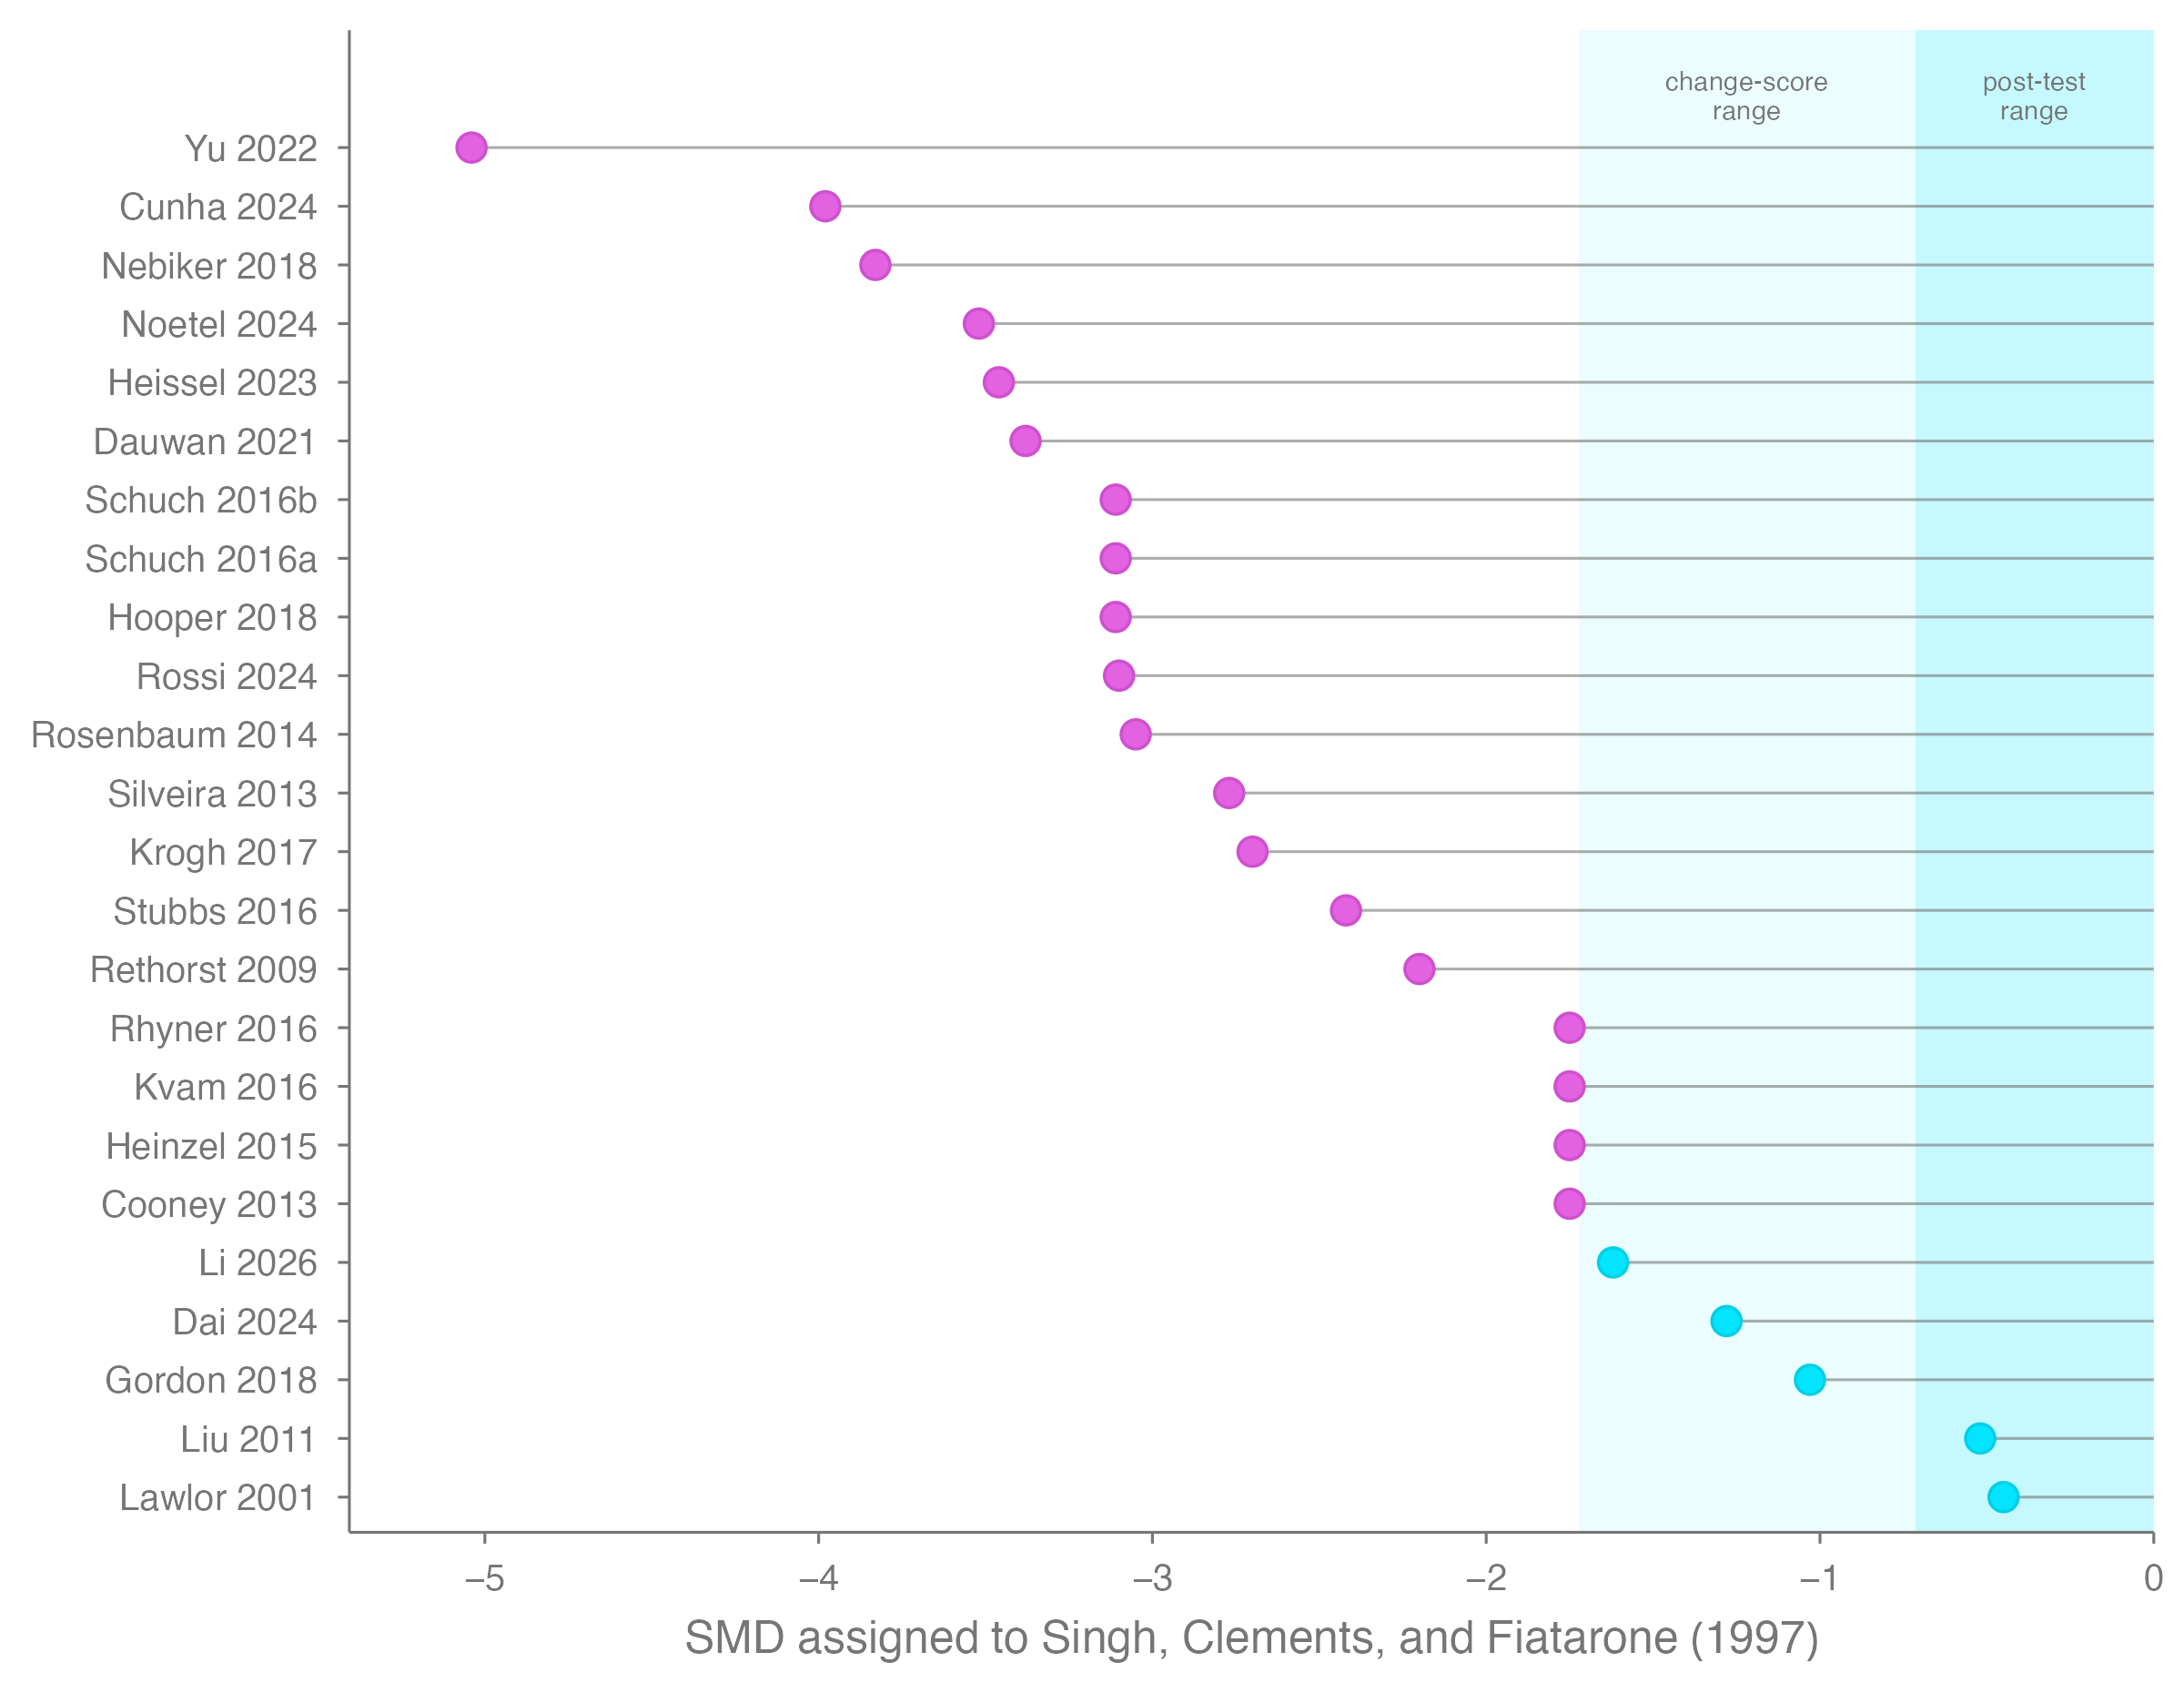
\includegraphics[keepaspectratio]{index_files/figure-pdf/fig-ma-effects-1.png}}

}

\caption{\label{fig-ma-effects}The effect size assigned to Singh,
Clements, and Fiatarone (1997) by each of the meta-analyses in
\hyperref[tbl-ma-effects]{Table~\ref*{tbl-ma-effects}}. Negative values
favor exercise. The blue ribbon covers the range of post-test SMDs (0 to
−0.72) that the article's own numbers support on any depression outcome.
The lighter ribbon extends that range to the largest change-score SMD
standardized by the baseline SD (−1.72). Blue points are defensible
extractions. Magenta points fall beyond any defensible extraction.}

\end{figure}%

Two forest plots, the figures in which a meta-analysis lists each
study's effect size beside the pooled estimate, show where this trial's
effect sits inside a published synthesis. In the meta-analysis of
exercise for depression in older adults by Cunha
(\citeproc{ref-cunha2024}{2024}), this trial enters three times, as
``Singh et al., 1997a'', ``1997b.1'', and ``1997b.2'', with effect sizes
of −3.02, −3.55, and −3.98
(\hyperref[fig-cunha]{Figure~\ref*{fig-cunha}}). These are the three
largest effects in the analysis, where the next largest is −1.34 and the
pooled estimate is −0.94. In the meta-analysis of neuromuscular exercise
interventions by Nebiker (\citeproc{ref-nebiker2018}{2018}), this trial
has an effect of −3.83 and a control group of 19 subjects, four more
than the trial had (\hyperref[fig-nebiker]{Figure~\ref*{fig-nebiker}}).
This entry is the largest effect in the analysis, more than twice the
next largest.

\begin{figure}[H]

\centering{

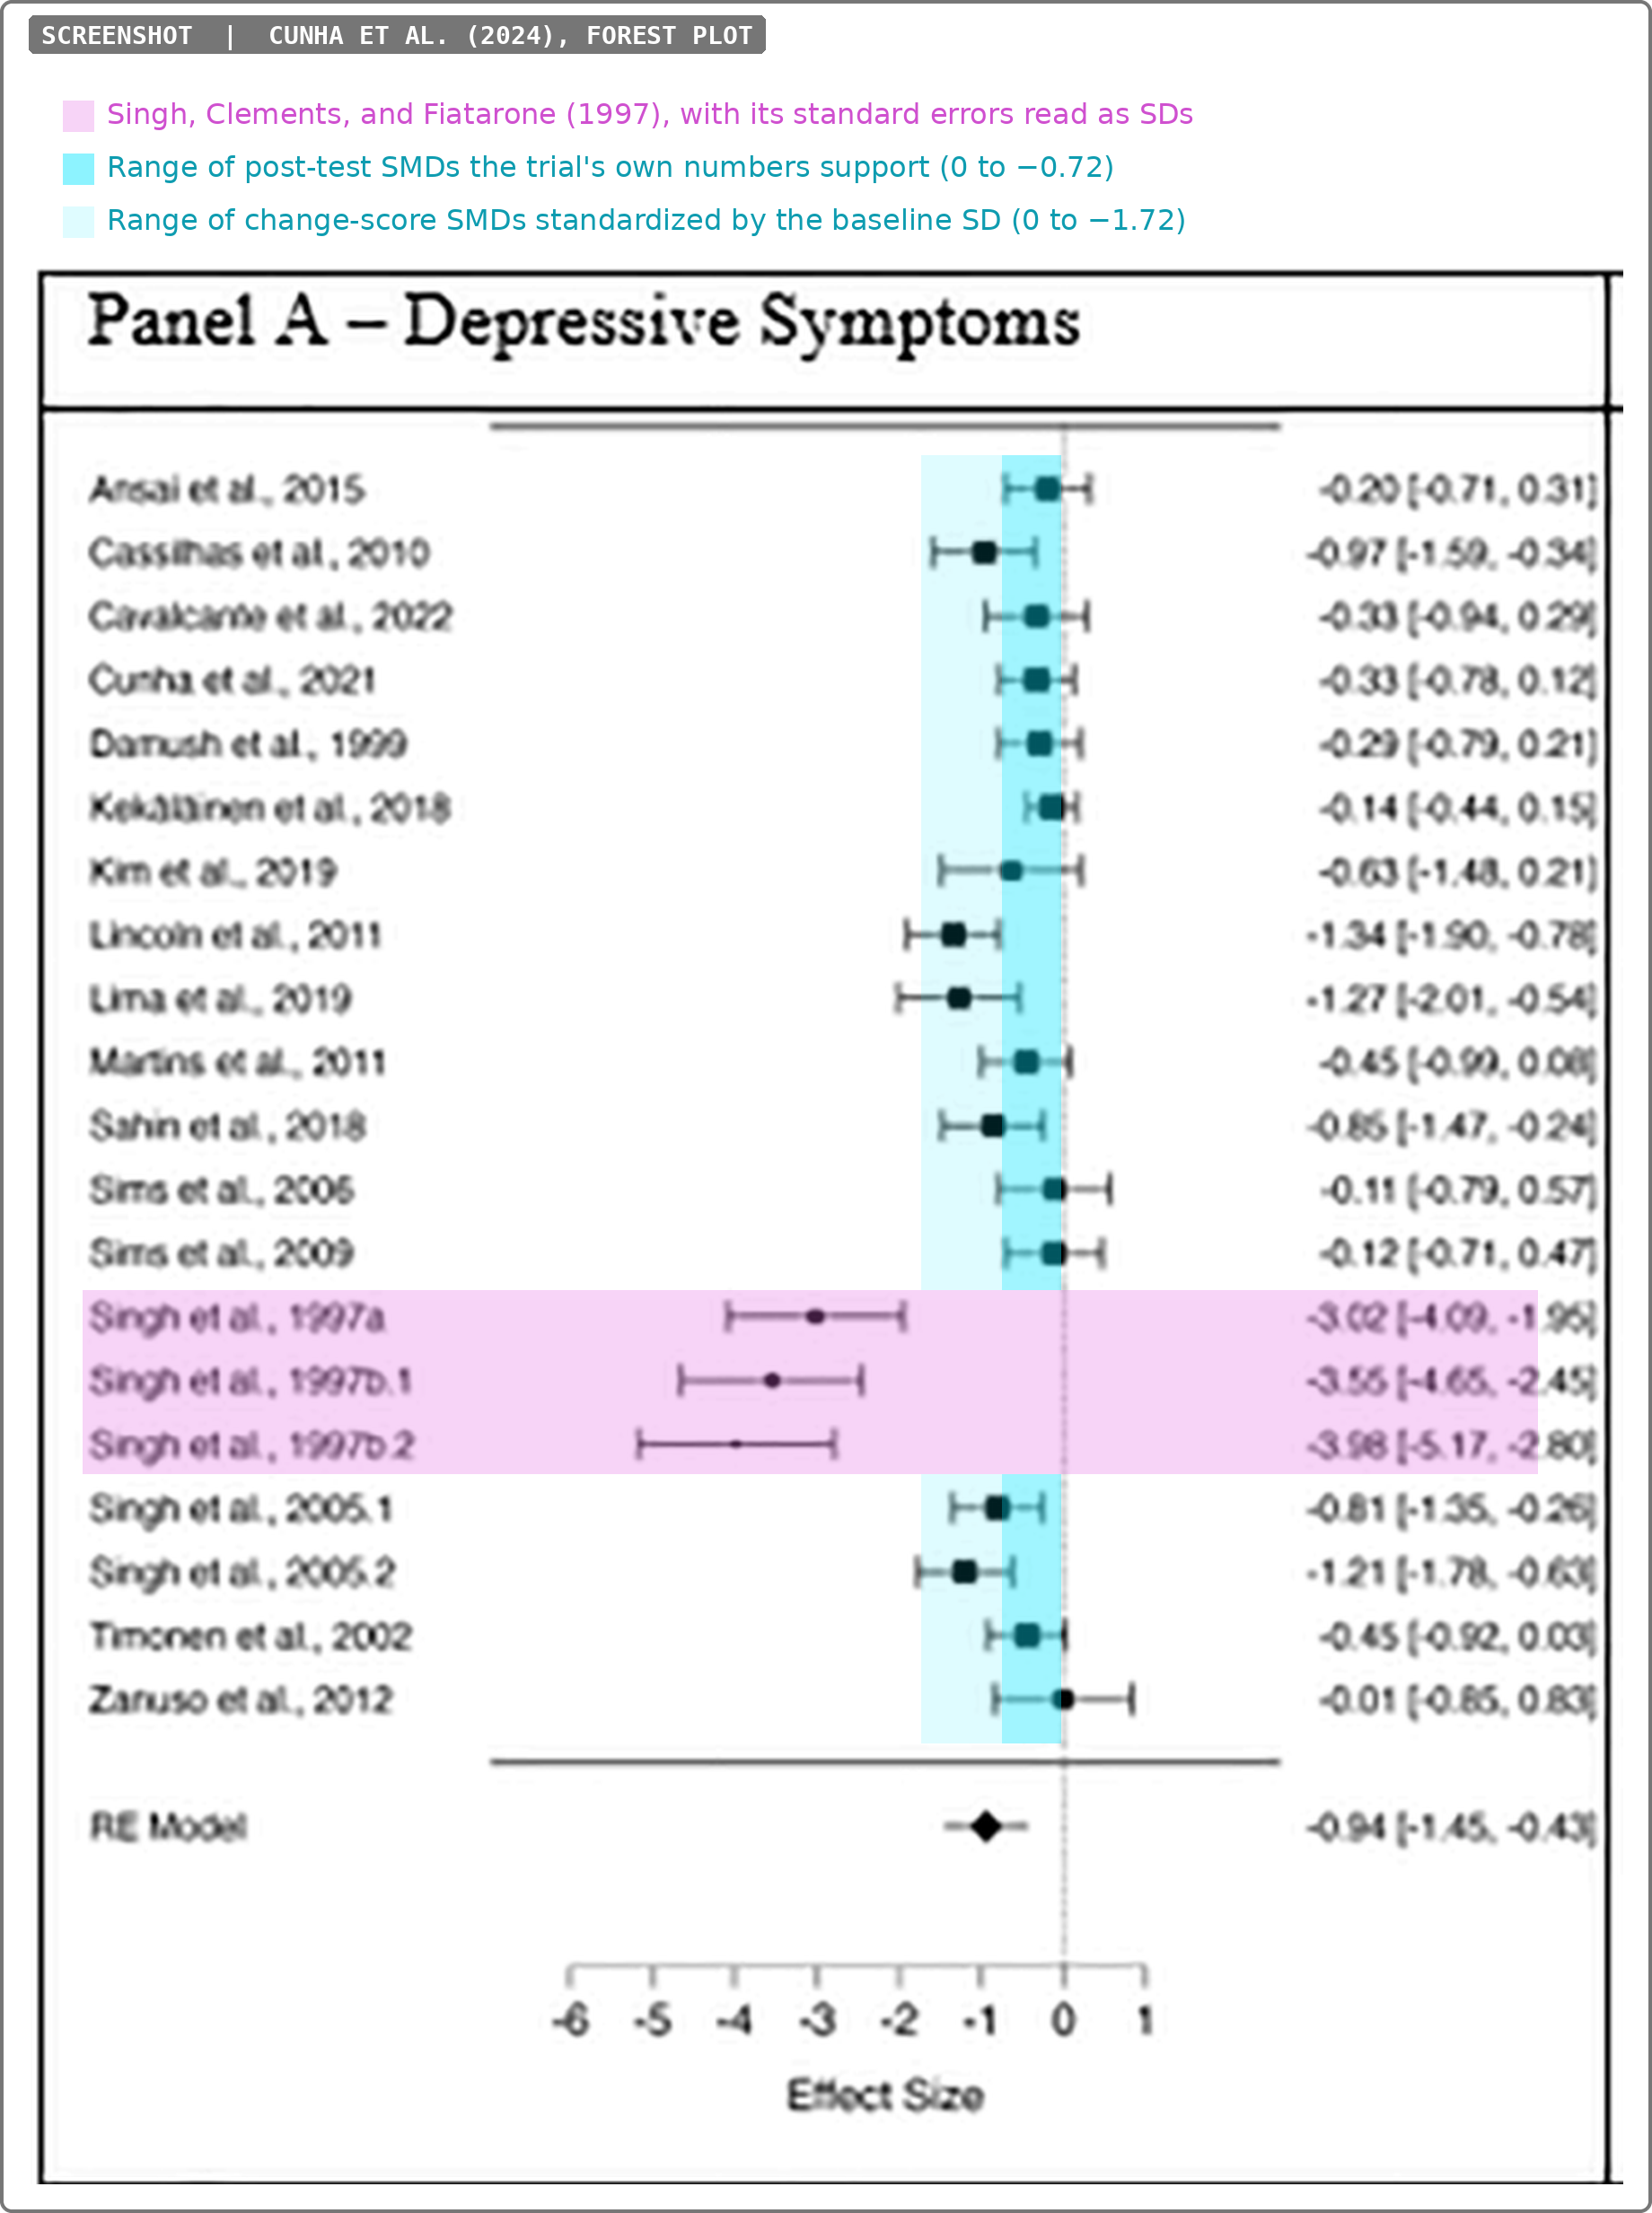
\includegraphics[width=0.78\linewidth,height=\textheight,keepaspectratio]{images/Cunha2024_forest_annotated.png}

}

\caption{\label{fig-cunha}The forest plot from Cunha
(\citeproc{ref-cunha2024}{2024}) for depressive symptoms, annotated. The
three entries for this trial are highlighted. The darker band marks the
range of post-test SMDs that a correct extraction of the article can
reach, and the lighter band the range that a change-score SMD
standardized by the baseline SD can reach (0 to −1.72).}

\end{figure}%

\begin{figure}[H]

\centering{

\pandocbounded{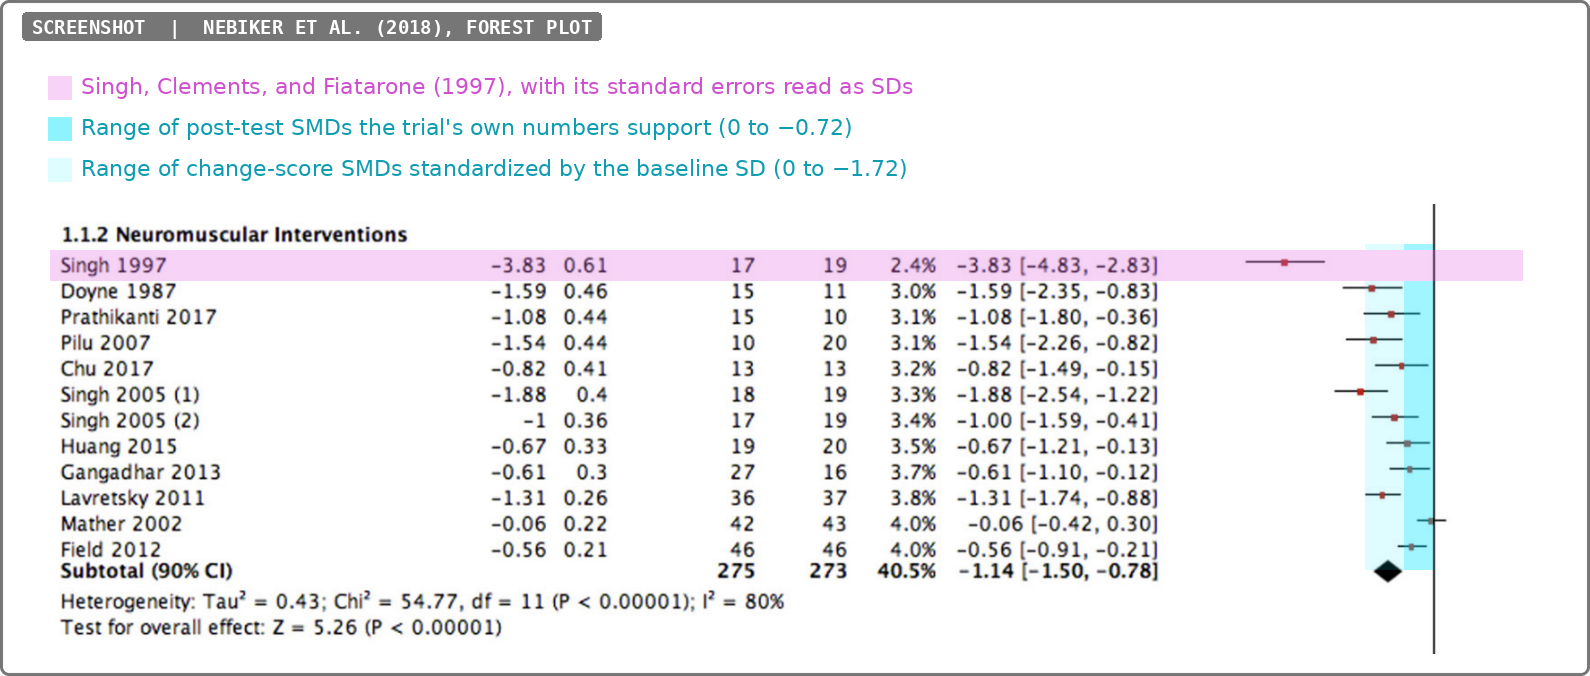
\includegraphics[keepaspectratio]{images/Nebiker2018_forest_annotated.png}}

}

\caption{\label{fig-nebiker}The neuromuscular interventions subgroup of
the forest plot from Nebiker (\citeproc{ref-nebiker2018}{2018}),
annotated in the same way. This trial is the first row.}

\end{figure}%

For nearly three decades, the evidence base on exercise as a treatment
for depression has carried this small trial as one of its largest
effects. Read correctly, the trial shows a moderate effect, but its
tables label the standard errors as standard deviations and
meta-analysts extracted them as labeled.

\subsection{Summary of findings}\label{summary-of-findings}

The values in parentheses throughout the article are standard errors,
although every table labels them as standard deviations. The article's
own age ranges, subgroup means, and test statistics show this
(\hyperref[sec-se-sd]{Section~\ref*{sec-se-sd}}). Read as labeled, the
trial's effect on depression is about four times larger than the data
support. Of the 24 meta-analyses we located, 19 carry the inflated
effect. Separately, the column labeled ``Baseline \emph{p}-value'' in
the outcome tables does not report baseline comparisons, 8 other
reported \emph{p} values can not be reproduced under any reading, two
reported SDs are impossible given their ranges, and one subgroup mean is
impossible given its sample size
(\hyperref[sec-unrecoverable]{Section~\ref*{sec-unrecoverable}}). In
total, this audit identifies 110 instances of Research Integrity
Violations. We recommend retraction
(\hyperref[sec-conclusion]{Section~\ref*{sec-conclusion}}).

\section{The values in parentheses are standard errors}\label{sec-se-sd}

Findings in this report are labeled using version 1.0 of the
\href{https://auditclinicalevidence.org/riv.html}{ACE Research Integrity
Violations taxonomy (ACE-RIV)}. A reported value that is wrong as
labeled but consistent with the rest of the article once the statistic
is read as what it actually is (here, a standard error labeled as a
standard deviation) is recorded under RIV 2.4, Data Miscalculation or
Erroneous Reporting. A reported value that no reading makes consistent
with the article's other numbers, such as a \emph{p} value that no test
of the reported data can return or an SD larger than its range allows,
is recorded under RIV 2.2, Statistical Inconsistencies and Impossible
Data Sets. Every finding in this section is recorded under RIV 2.4.

\subsection{The labels and the Methods disagree}\label{sec-labels}

Tables 1, 2, 3, 4, 6, and 7 of Singh (\citeproc{ref-singh1997}{1997})
report the summary statistics for the baseline characteristics and
outcomes. The footnote of each of these tables states that the values
are ``Means and (\emph{SD})''. Yet the statistical analysis section of
the Methods states that they are standard errors (see
\hyperref[fig-methods]{Figure~\ref*{fig-methods}}).

\begin{quote}
Continuous data are described as the mean (standard error) or median and
range as appropriate, except for quality of life measures which are
presented as mean (standard deviation) to allow comparison with reported
normal values.
\end{quote}

Both statements can not be true, but the article reports enough to
determine which one is correct.

\begin{figure}[H]

\centering{

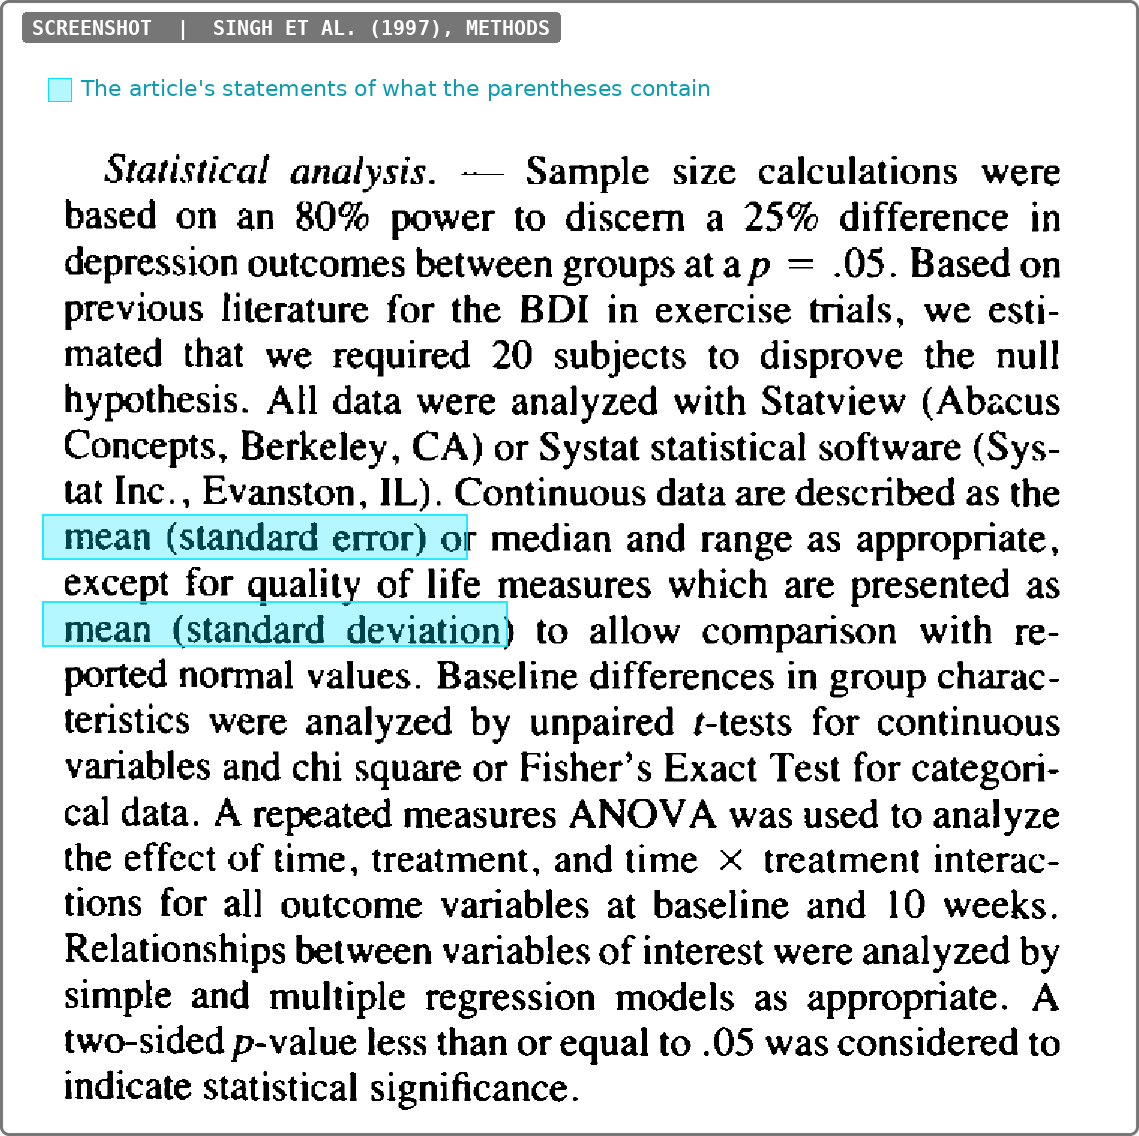
\includegraphics[width=0.7\linewidth,height=\textheight,keepaspectratio]{images/singh_methods_annotated.png}

}

\caption{\label{fig-methods}The statistical analysis paragraph of the
Methods of Singh (\citeproc{ref-singh1997}{1997}). Blue marks the two
statements of what the parentheses contain, standard errors for
continuous data and standard deviations for the quality of life
measures.}

\end{figure}%

\subsection{Values that can not be standard
deviations}\label{sec-not-sd}

Beneath the mean age of each group, Table 1 reports the age range, 61 to
82 years in the exercise group and 60 to 84 years in the control group.
A standard deviation limits how far apart the youngest and oldest
subjects can be. The widest range a group can have for a given SD arises
when one subject sits at each end of the range and every other subject
sits exactly at the mean, because that arrangement spreads the ages as
far as possible while adding the least to the SD. For a group of \(n\)
subjects with standard deviation \(s\), that widest possible range is
\(s\sqrt{2(n-1)}\). A reported range wider than this can not come from a
group with that SD. If the value of 1.5 for the exercise group is an SD,
even one as large as 1.55 before rounding, the ages of its 17 subjects
could span at most 8.8 years, against a reported span of 21 years. If
the value of 2.0 for the control group is an SD, the ages of its 15
subjects could span at most 10.8 years, against a reported 24 years. If
the value of 1.2 in the abstract is an SD, the ages of all 32 subjects
could span at most 9.8 years, against a reported 24 years. The values in
parentheses can not be SDs. If they are standard errors (SEs), the
implied SDs are 6.2, 7.7, and 6.8 years, which fit the reported ranges.

\begin{figure}[H]

\centering{

\pandocbounded{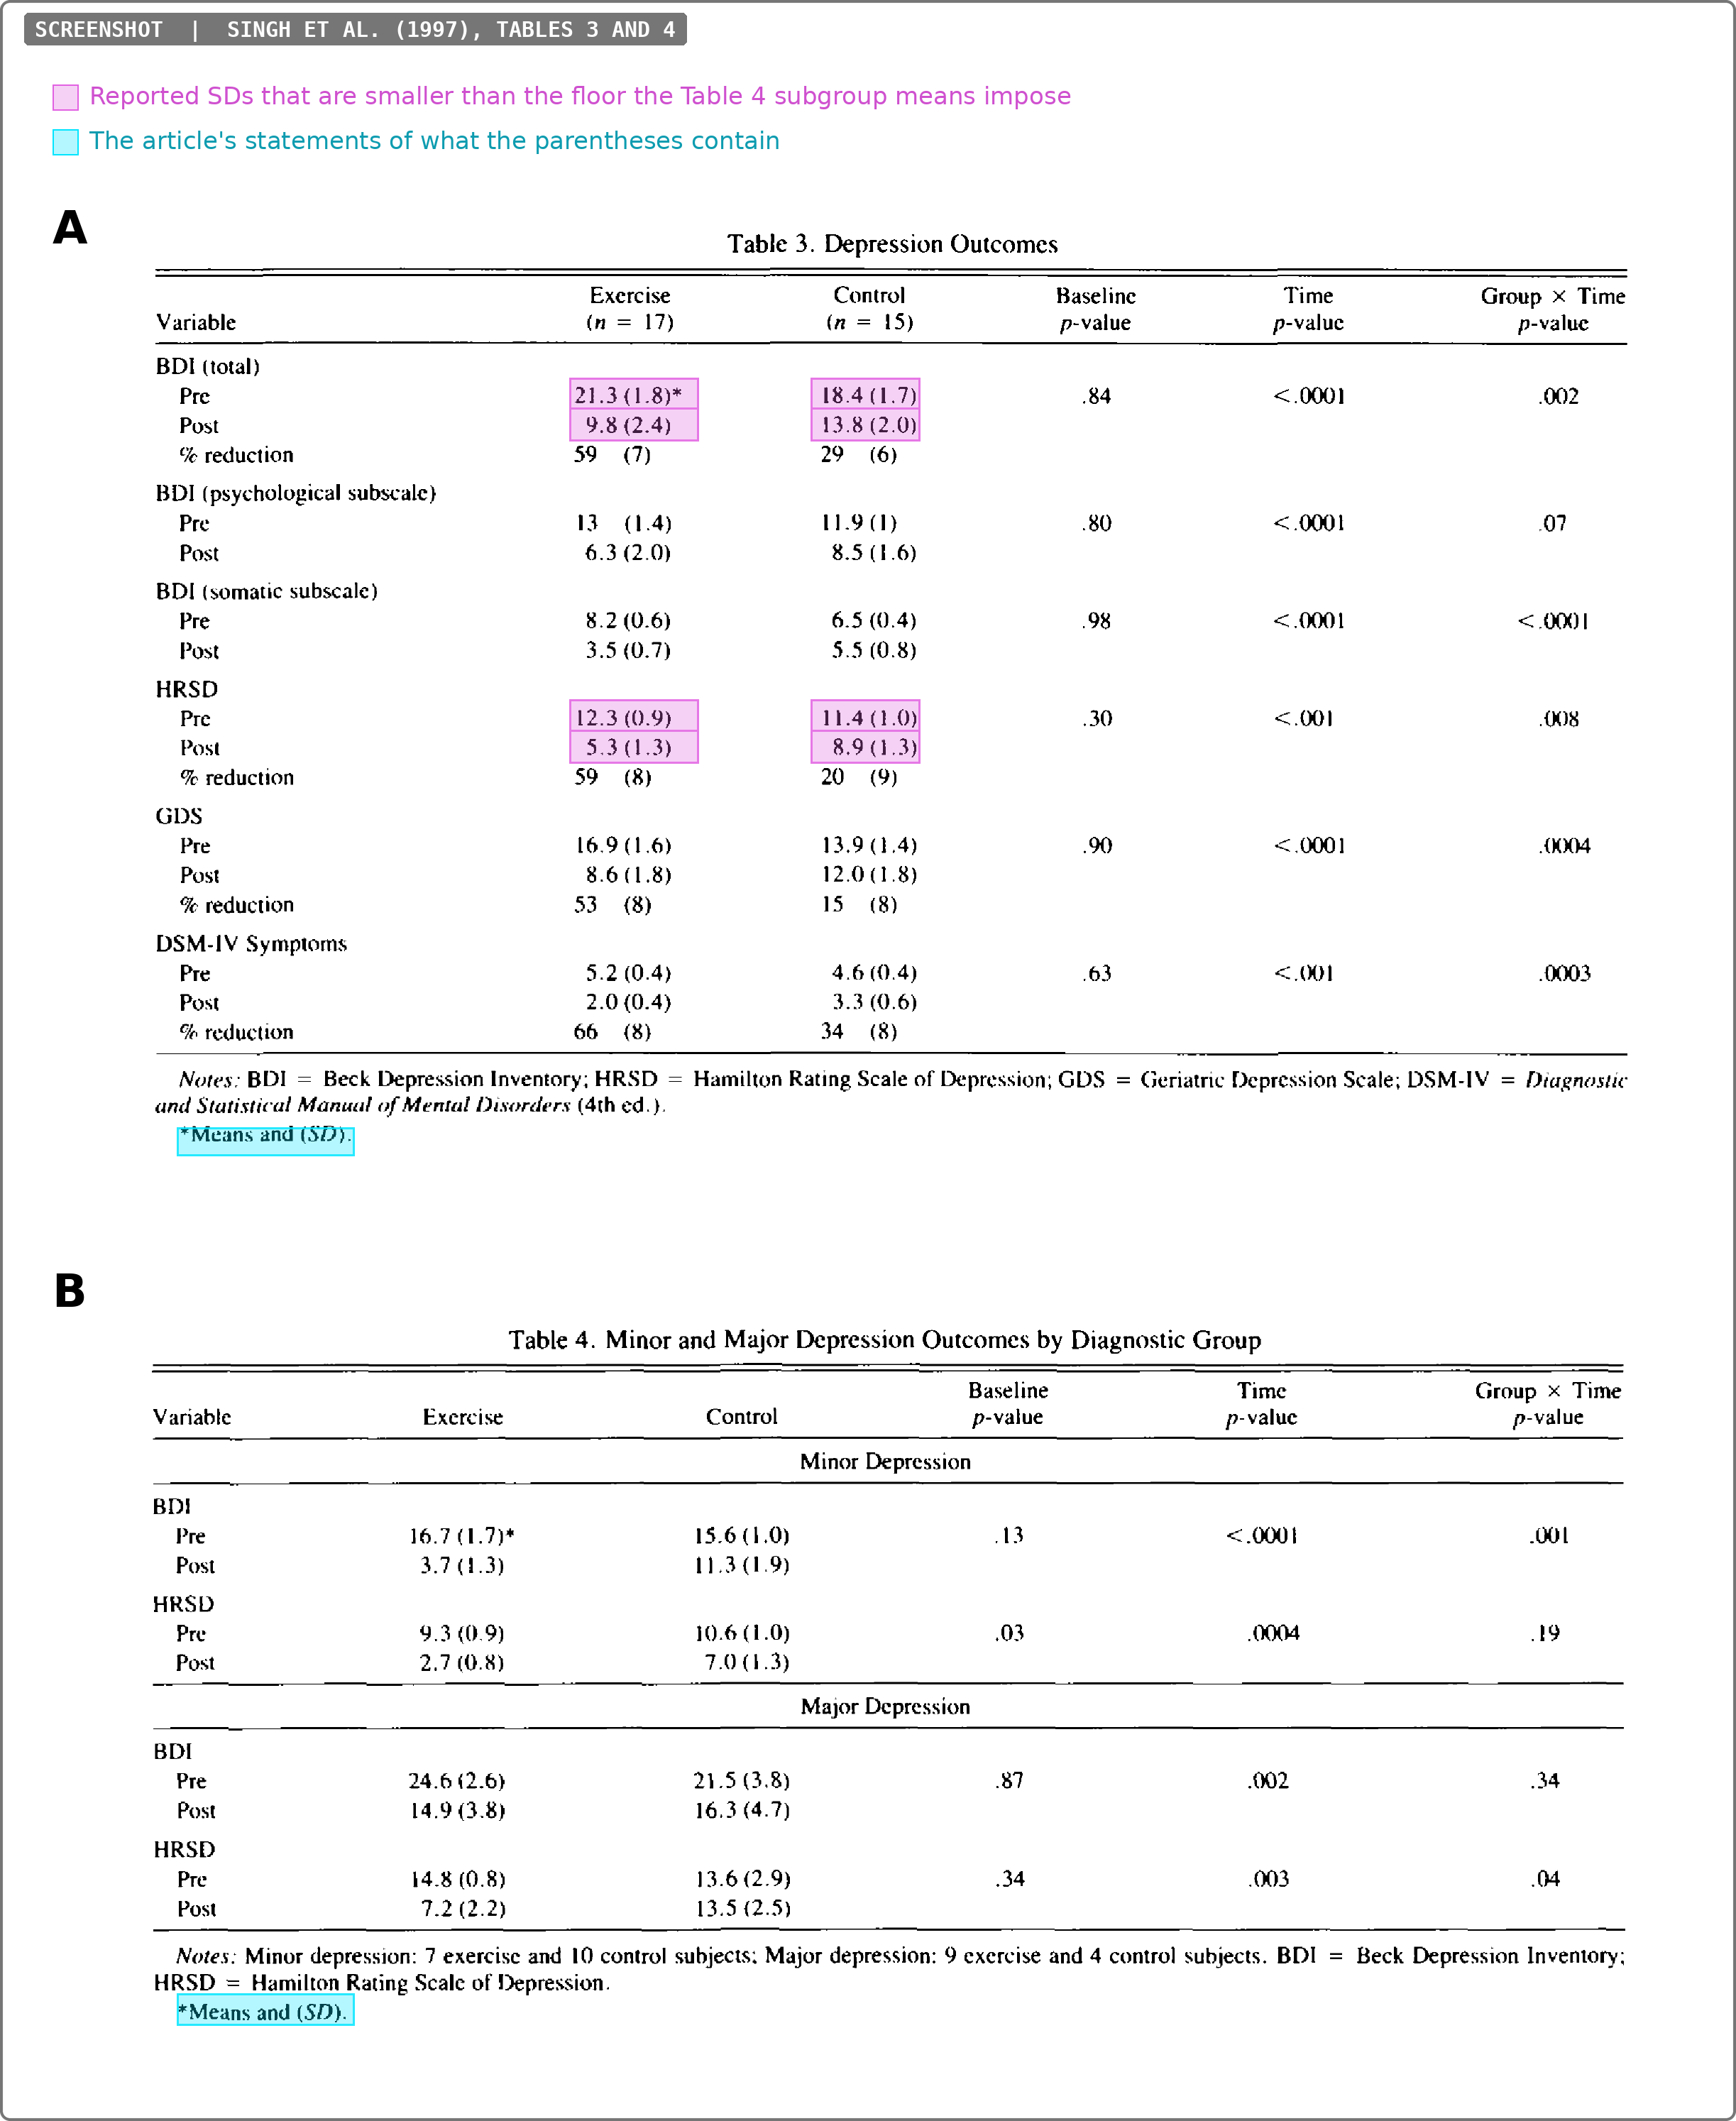
\includegraphics[keepaspectratio]{images/singh_tables_3_4_annotated.png}}

}

\caption{\label{fig-tables-3-4}Panel A shows Table 3 of Singh
(\citeproc{ref-singh1997}{1997}), the depression outcomes for the whole
groups. Panel B shows Table 4, the same outcomes by diagnostic subgroup.
Pink marks the BDI and HRSD parentheticals in Table 3, every one of
which is below the smallest standard deviation that the subgroup means
in Table 4 allow. Blue marks the footnotes stating what the parentheses
contain.}

\end{figure}%

The outcome tables can also be checked against each other, because Table
4 breaks the BDI and HRSD outcomes of Table 3 down by diagnostic
subgroup, with 7 exercise and 10 control subjects with minor depression
and 9 exercise and 4 control subjects with major depression (see panel B
of \hyperref[fig-tables-3-4]{Figure~\ref*{fig-tables-3-4}}). The one
dysthymic subject in each group is in neither subgroup. The variance of
a whole group (the square of its SD) equals the variance within the
subgroups plus the variance between the subgroup means. Neither part can
be negative, so the spread of the subgroup means alone puts a lower
bound on the SD of the whole group, whatever the spread within each
subgroup. For the exercise group at baseline, the subgroup BDI means of
16.7 and 24.6 around a whole-group mean of 21.3 require a whole-group SD
of at least 3.87. Table 3 reports 1.8. This bound holds with every
reported mean free to fall anywhere within its rounding interval (the
values that round to the reported one, 21.25 to 21.35 for a reported
21.3), in whichever direction lowers the bound, with the reported value
taken at the top of its own interval, and with the dysthymic subject
ignored. The same calculation for all 8 BDI and HRSD values in Table 3
gives lower bounds from 1.31 to 5.51, and every reported value, from 0.9
to 2.4, is below its bound. None of these values can be SDs. Read as
SEs, the implied SDs, from 3.7 to 9.9, are all above their bounds.

\subsection{\texorpdfstring{Reported \emph{p} values reproduce only as
standard
errors}{Reported p values reproduce only as standard errors}}\label{sec-sdse}

Every reported \emph{p} value in these tables can be recalculated from
the reported means, the values in parentheses, and the group sizes. We
recalculated each one twice, once reading the values in parentheses as
standard deviations (SDs) and once as standard errors (SEs). Every
reported value is rounded, so each mean and parenthetical value may sit
anywhere in its rounding interval. Table 1 and Table 2 report unpaired
comparisons, which we tested with Student's and Welch's \emph{t} tests.
Each outcome table reports a Group × Time \emph{p} value for every
variable, which tests whether the two groups changed by different
amounts over the 10 weeks. In a repeated measures ANOVA with two groups
and two time points, that \emph{p} value is the \emph{t} test comparing
the change scores (each subject's 10-week score minus their baseline
score) of the two groups. The SD of a change score depends on the
correlation between the baseline and 10-week scores, which the article
does not report. We therefore let that correlation take any value from
−1 to 1, separately in each group, which gives the widest range of
\emph{p} values each reading could produce. Allowing every correlation
can only make the test more lenient. Under either reading the range runs
from near zero, where the correlation is close to 1 and the change
scores are tightly clustered, up to a ceiling set by a correlation of
−1, where they are most spread out. A reading is ruled out only when the
reported \emph{p} value lies above that ceiling, so that no correlation
could have produced it. Each range is rounded outward to the precision
of the reported value. A reading is possible when the reported \emph{p}
value falls inside its range (see
\hyperref[tbl-sdse-a]{Table~\ref*{tbl-sdse-a}} and
\hyperref[tbl-sdse-b]{Table~\ref*{tbl-sdse-b}}). Table 5 serves as a
check on the method, because the Methods identify its parenthetical
values as SDs. Read as SDs, all 8 of its Group × Time \emph{p} values
reproduce, whereas three of them do not reproduce with the values read
as SEs.

For 25 variables in Tables 1, 2, 3, 4, 6, and 7, no reading of the
parenthetical values as SDs can return the reported \emph{p} value,
whereas every one of them reproduces with the values read as SEs. For
medications per day in Table 1, the SD reading gives .00--.01 against a
reported .36, and the SE reading gives .25--.46. For HRSD in Table 3,
the SD reading gives .000--.001 against a reported .008. For lifting
self-efficacy in Table 6, it gives .00--.55 against a reported .59. For
the other variables the test does not separate the two readings, either
because the reported \emph{p} value is very small or very large or
because the range under the SD reading is wide enough to contain it. ADL
in Table 7 reproduces only as SDs, because the control group's baseline
parenthetical value of 0.1 is far smaller than the other three values in
the row (0.8, 0.8, and 0.9). It is described but not counted.

\begin{table}

\caption{\label{tbl-sdse-a}Reported p-values in Tables 1 through 4
against the p-values each reading of the parenthetical values can
produce.}

\centering{

\centering
\begin{talltblr}[         %% tabularray outer open
entry=none,label=none,
note{}={\textit{Note.} Unpaired is Student's and Welch's two-sample t tests. Group × Time is the t test on change scores, which is the interaction of a two-group, two-time repeated measures ANOVA. Its range allows any pre-post correlation from −1 to 1 in each group. Every mean and parenthetical value may sit anywhere in its rounding interval, and each range is rounded outward to the precision of the reported value. As SD uses the parenthetical values as reported. As SE multiplies each by the square root of its group size (exercise 17, control 15, or 14 in Table 7, and the subgroup sizes in Table 4). Possible is No when the reported p-value falls outside the range that reading can produce.},
]                     %% tabularray outer close
{                     %% tabularray inner open
colspec={Q[]Q[]Q[]Q[]Q[]Q[]Q[]},
cell{1,4-10,12-15,17-22,24-27}{1}={}{font=\fontsize{0.9em}{1.2em}\selectfont,},
cell{1,4-10,12-15,17-22,24-27}{2}={}{halign=c, font=\fontsize{0.9em}{1.2em}\selectfont,},
cell{1,4-10,12-15,17-22,24-27}{3}={}{halign=c, font=\fontsize{0.9em}{1.2em}\selectfont,},
cell{1,4-10,12-15,17-22,24-27}{5}={}{halign=c, font=\fontsize{0.9em}{1.2em}\selectfont,},
cell{1}{4}={c=2,}{halign=c, font=\fontsize{0.9em}{1.2em}\selectfont, halign=c,},
cell{1}{6}={}{halign=c, font=\fontsize{0.9em}{1.2em}\selectfont,},
cell{1}{7}={}{halign=c, font=\fontsize{0.9em}{1.2em}\selectfont,},
cell{12,19,24,26}{6}={}{halign=c, font=\fontsize{0.9em}{1.2em}\selectfont, fg=c0e9cb0,},
cell{2}{1}={}{font=\fontsize{0.9em}{1.2em}\selectfont, font=\ttfamily, fg=c767676, font=\fontsize{0.85em}{1.15em}\selectfont, font=\ttfamily, fg=c767676, font=\fontsize{0.85em}{1.15em}\selectfont,},
cell{2}{2}={}{halign=c, font=\fontsize{0.9em}{1.2em}\selectfont, font=\ttfamily, fg=c767676, font=\fontsize{0.85em}{1.15em}\selectfont, font=\ttfamily, fg=c767676, font=\fontsize{0.85em}{1.15em}\selectfont,},
cell{2}{3}={}{halign=c, font=\fontsize{0.9em}{1.2em}\selectfont, font=\ttfamily, fg=c767676, font=\fontsize{0.85em}{1.15em}\selectfont, font=\ttfamily, fg=c767676, font=\fontsize{0.85em}{1.15em}\selectfont,},
cell{2}{4}={}{halign=c, font=\fontsize{0.9em}{1.2em}\selectfont, font=\ttfamily, fg=c767676, font=\fontsize{0.85em}{1.15em}\selectfont, font=\ttfamily, fg=c767676, font=\fontsize{0.85em}{1.15em}\selectfont,},
cell{2}{5}={}{halign=c, font=\fontsize{0.9em}{1.2em}\selectfont, font=\ttfamily, fg=c767676, font=\fontsize{0.85em}{1.15em}\selectfont, font=\ttfamily, fg=c767676, font=\fontsize{0.85em}{1.15em}\selectfont,},
cell{2}{6}={}{halign=c, font=\fontsize{0.9em}{1.2em}\selectfont, font=\ttfamily, fg=c767676, font=\fontsize{0.85em}{1.15em}\selectfont, font=\ttfamily, fg=c767676, font=\fontsize{0.85em}{1.15em}\selectfont,},
cell{2}{7}={}{halign=c, font=\fontsize{0.9em}{1.2em}\selectfont, font=\ttfamily, fg=c767676, font=\fontsize{0.85em}{1.15em}\selectfont, font=\ttfamily, fg=c767676, font=\fontsize{0.85em}{1.15em}\selectfont,},
cell{3,11,16,23}{1}={c=7,}{font=\itshape, font=\fontsize{0.9em}{1.2em}\selectfont,},
cell{3,11,16,23}{2}={}{font=\itshape, halign=c, font=\fontsize{0.9em}{1.2em}\selectfont,},
cell{3,11,16,23}{3}={}{font=\itshape, halign=c, font=\fontsize{0.9em}{1.2em}\selectfont,},
cell{3,11,16,23}{4}={}{font=\itshape, halign=c, font=\fontsize{0.9em}{1.2em}\selectfont,},
cell{3,11,16,23}{5}={}{font=\itshape, halign=c, font=\fontsize{0.9em}{1.2em}\selectfont,},
cell{3,11,16,23}{6}={}{font=\itshape, halign=c, font=\fontsize{0.9em}{1.2em}\selectfont,},
cell{3,11,16,23}{7}={}{font=\itshape, halign=c, font=\fontsize{0.9em}{1.2em}\selectfont,},
cell{4-10,12-15,17-22,24-27}{4}={}{halign=c, font=\fontsize{0.9em}{1.2em}\selectfont,},
cell{4-10,13-15,17-18,20-22,25,27}{6}={}{halign=c, font=\fontsize{0.9em}{1.2em}\selectfont, font=\bfseries, fg=ccf50cf, bg=cfbe4fb,},
cell{4-5,7-9,12-13,15,17-22,24-27}{7}={}{halign=c, font=\fontsize{0.9em}{1.2em}\selectfont, fg=c0e9cb0,},
cell{6,10,14}{7}={}{halign=c, font=\fontsize{0.9em}{1.2em}\selectfont, font=\bfseries, fg=ccf50cf, bg=cfbe4fb,},
}                     %% tabularray inner close
\tinytableDefineColor{c767676}{HTML}{767676}
\tinytableDefineColor{cfbe4fb}{HTML}{fbe4fb}
\tinytableDefineColor{ccf50cf}{HTML}{cf50cf}
\tinytableDefineColor{c0e9cb0}{HTML}{0e9cb0}
\toprule
&  &  & Reproduced \textit{p} &  &  &  \\ \cmidrule[lr]{4-5}
Variable & Test & Reported \textit{p} & As SD & As SE & Possible as SD & Possible as SE \\ \midrule %% TinyTableHeader
Table 1, baseline characteristics &  &  &  &  &  &  \\
Age (years) & Unpaired & .34 & .00–.14 & .21–.71 & No & Yes \\
Education (years) & Unpaired & .65 & .02–.18 & .55–.73 & No & Yes \\
Ethanol (g per day) & Unpaired & .34 & .02–.07 & .56–.63 & No & No \\
Medications per day & Unpaired & .36 & .00–.01 & .25–.46 & No & Yes \\
Chronic diseases & Unpaired & .10 & .00–.01 & .01–.17 & No & Yes \\
Mini-Mental State Exam & Unpaired & .70 & .00–.50 & .48–.87 & No & Yes \\
Duration of symptoms (months) & Unpaired & .45 & .01–.06 & .50–.62 & No & No \\
Table 2, adverse events &  &  &  &  &  &  \\
Visits to a health professional & Unpaired & .90 & .16–1.00 & .72–1.00 & Yes & Yes \\
Minor illness & Unpaired & .50 & .00–.07 & .37–.64 & No & Yes \\
Hospital days & Unpaired & .40 & .00–.05 & .41–.60 & No & No \\
Musculoskeletal pain & Unpaired & .80 & .20–.71 & .74–.93 & No & Yes \\
Table 3, depression outcomes &  &  &  &  &  &  \\
BDI total & Group × Time & .002 & .000–.001 & .000–.258 & No & Yes \\
BDI psychological & Group × Time & .07 & .00–.04 & .00–.59 & No & Yes \\
BDI somatic & Group × Time & <.0001 & .0000–.0001 & .0000–.0794 & Yes & Yes \\
HRSD & Group × Time & .008 & .000–.001 & .000–.207 & No & Yes \\
GDS & Group × Time & .0004 & .0000–.0001 & .0000–.2108 & No & Yes \\
DSM-IV symptoms & Group × Time & .0003 & .0000–.0001 & .0000–.2370 & No & Yes \\
Table 4, diagnostic subgroups &  &  &  &  &  &  \\
Minor depression, BDI & Group × Time & .001 & .000–.001 & .000–.075 & Yes & Yes \\
Minor depression, HRSD & Group × Time & .19 & .00–.02 & .00–.41 & No & Yes \\
Major depression, BDI & Group × Time & .34 & .00–.34 & .02–.72 & Yes & Yes \\
Major depression, HRSD & Group × Time & .04 & .00–.01 & .00–.25 & No & Yes \\
\bottomrule
\end{talltblr}

}

\end{table}%

\begin{table}

\caption{\label{tbl-sdse-b}Reported p-values in Tables 5 through 7
against the p-values each reading of the parenthetical values can
produce. Table 5 is the control, the one table whose values the Methods
identify as standard deviations.}

\centering{

\centering
\begin{talltblr}[         %% tabularray outer open
entry=none,label=none,
note{}={\textit{Note.} Unpaired is Student's and Welch's two-sample t tests. Group × Time is the t test on change scores, which is the interaction of a two-group, two-time repeated measures ANOVA. Its range allows any pre-post correlation from −1 to 1 in each group. Every mean and parenthetical value may sit anywhere in its rounding interval, and each range is rounded outward to the precision of the reported value. As SD uses the parenthetical values as reported. As SE multiplies each by the square root of its group size (exercise 17, control 15, or 14 in Table 7, and the subgroup sizes in Table 4). Possible is No when the reported p-value falls outside the range that reading can produce.},
]                     %% tabularray outer close
{                     %% tabularray inner open
colspec={Q[]Q[]Q[]Q[]Q[]Q[]Q[]},
cell{1,4-11,13-21,23-30}{1}={}{font=\fontsize{0.9em}{1.2em}\selectfont,},
cell{1,4-11,13-21,23-30}{2}={}{halign=c, font=\fontsize{0.9em}{1.2em}\selectfont,},
cell{1,4-11,13-21,23-30}{3}={}{halign=c, font=\fontsize{0.9em}{1.2em}\selectfont,},
cell{1,4-11,13-21,23-30}{5}={}{halign=c, font=\fontsize{0.9em}{1.2em}\selectfont,},
cell{1}{4}={c=2,}{halign=c, font=\fontsize{0.9em}{1.2em}\selectfont, halign=c,},
cell{1}{6}={}{halign=c, font=\fontsize{0.9em}{1.2em}\selectfont,},
cell{1}{7}={}{halign=c, font=\fontsize{0.9em}{1.2em}\selectfont,},
cell{13-20,27-29}{6}={}{halign=c, font=\fontsize{0.9em}{1.2em}\selectfont, font=\bfseries, fg=ccf50cf, bg=cfbe4fb,},
cell{2}{1}={}{font=\fontsize{0.9em}{1.2em}\selectfont, font=\ttfamily, fg=c767676, font=\fontsize{0.85em}{1.15em}\selectfont, font=\ttfamily, fg=c767676, font=\fontsize{0.85em}{1.15em}\selectfont,},
cell{2}{2}={}{halign=c, font=\fontsize{0.9em}{1.2em}\selectfont, font=\ttfamily, fg=c767676, font=\fontsize{0.85em}{1.15em}\selectfont, font=\ttfamily, fg=c767676, font=\fontsize{0.85em}{1.15em}\selectfont,},
cell{2}{3}={}{halign=c, font=\fontsize{0.9em}{1.2em}\selectfont, font=\ttfamily, fg=c767676, font=\fontsize{0.85em}{1.15em}\selectfont, font=\ttfamily, fg=c767676, font=\fontsize{0.85em}{1.15em}\selectfont,},
cell{2}{4}={}{halign=c, font=\fontsize{0.9em}{1.2em}\selectfont, font=\ttfamily, fg=c767676, font=\fontsize{0.85em}{1.15em}\selectfont, font=\ttfamily, fg=c767676, font=\fontsize{0.85em}{1.15em}\selectfont,},
cell{2}{5}={}{halign=c, font=\fontsize{0.9em}{1.2em}\selectfont, font=\ttfamily, fg=c767676, font=\fontsize{0.85em}{1.15em}\selectfont, font=\ttfamily, fg=c767676, font=\fontsize{0.85em}{1.15em}\selectfont,},
cell{2}{6}={}{halign=c, font=\fontsize{0.9em}{1.2em}\selectfont, font=\ttfamily, fg=c767676, font=\fontsize{0.85em}{1.15em}\selectfont, font=\ttfamily, fg=c767676, font=\fontsize{0.85em}{1.15em}\selectfont,},
cell{2}{7}={}{halign=c, font=\fontsize{0.9em}{1.2em}\selectfont, font=\ttfamily, fg=c767676, font=\fontsize{0.85em}{1.15em}\selectfont, font=\ttfamily, fg=c767676, font=\fontsize{0.85em}{1.15em}\selectfont,},
cell{3,12,22}{1}={c=7,}{font=\itshape, font=\fontsize{0.9em}{1.2em}\selectfont,},
cell{3,12,22}{2}={}{font=\itshape, halign=c, font=\fontsize{0.9em}{1.2em}\selectfont,},
cell{3,12,22}{3}={}{font=\itshape, halign=c, font=\fontsize{0.9em}{1.2em}\selectfont,},
cell{3,12,22}{4}={}{font=\itshape, halign=c, font=\fontsize{0.9em}{1.2em}\selectfont,},
cell{3,12,22}{5}={}{font=\itshape, halign=c, font=\fontsize{0.9em}{1.2em}\selectfont,},
cell{3,12,22}{6}={}{font=\itshape, halign=c, font=\fontsize{0.9em}{1.2em}\selectfont,},
cell{3,12,22}{7}={}{font=\itshape, halign=c, font=\fontsize{0.9em}{1.2em}\selectfont,},
cell{4-11,13-21,23-30}{4}={}{halign=c, font=\fontsize{0.9em}{1.2em}\selectfont,},
cell{4-11,21,23-26,30}{6}={}{halign=c, font=\fontsize{0.9em}{1.2em}\selectfont, fg=c0e9cb0,},
cell{4-6,9-10,13-21,24-30}{7}={}{halign=c, font=\fontsize{0.9em}{1.2em}\selectfont, fg=c0e9cb0,},
cell{7-8,11,23}{7}={}{halign=c, font=\fontsize{0.9em}{1.2em}\selectfont, font=\bfseries, fg=ccf50cf, bg=cfbe4fb,},
}                     %% tabularray inner close
\tinytableDefineColor{c767676}{HTML}{767676}
\tinytableDefineColor{cfbe4fb}{HTML}{fbe4fb}
\tinytableDefineColor{ccf50cf}{HTML}{cf50cf}
\tinytableDefineColor{c0e9cb0}{HTML}{0e9cb0}
\toprule
&  &  & Reproduced \textit{p} &  &  &  \\ \cmidrule[lr]{4-5}
Variable & Test & Reported \textit{p} & As SD & As SE & Possible as SD & Possible as SE \\ \midrule %% TinyTableHeader
Table 5, quality of life (SDs according to the Methods) &  &  &  &  &  &  \\
Physical functioning & Group × Time & .22 & .00–.54 & .07–.88 & Yes & Yes \\
Role physical & Group × Time & .16 & .00–.46 & .02–.86 & Yes & Yes \\
Bodily pain & Group × Time & .001 & .000–.109 & .000–.680 & Yes & Yes \\
General health & Group × Time & .06 & .00–.51 & .23–.87 & Yes & No \\
Vitality & Group × Time & .002 & .000–.234 & .016–.763 & Yes & No \\
Social functioning & Group × Time & .008 & .000–.100 & .000–.674 & Yes & Yes \\
Role emotional & Group × Time & .02 & .00–.27 & .00–.78 & Yes & Yes \\
Mental health & Group × Time & .24 & .00–.66 & .32–.92 & Yes & No \\
Table 6, self-efficacy and morale &  &  &  &  &  &  \\
Lifting & Group × Time & .59 & .00–.55 & .00–.88 & No & Yes \\
Climbing & Group × Time & .63 & .00–.43 & .00–.85 & No & Yes \\
Pushups & Group × Time & .48 & .00–.28 & .00–.79 & No & Yes \\
Jogging & Group × Time & .25 & .00–.05 & .00–.61 & No & Yes \\
Walking & Group × Time & .14 & .00–.02 & .00–.53 & No & Yes \\
Philadelphia Geriatric Morale Scale & Group × Time & .03 & .00–.01 & .00–.39 & No & Yes \\
Agitation & Group × Time & .17 & .00–.04 & .00–.60 & No & Yes \\
Attitude toward aging & Group × Time & .04 & .00–.01 & .00–.33 & No & Yes \\
Loneliness & Group × Time & .30 & .00–.45 & .00–.85 & Yes & Yes \\
Table 7, function and performance &  &  &  &  &  &  \\
ADL & Group × Time & .36 & .08–1.00 & .63–1.00 & Yes & No \\
IADL & Group × Time & .80 & .00–1.00 & .00–1.00 & Yes & Yes \\
SIP total & Group × Time & .84 & .00–.90 & .43–.98 & Yes & Yes \\
Gait speed & Group × Time & .32 & .00–1.00 & .00–1.00 & Yes & Yes \\
6-minute walk & Group × Time & .36 & .00–.31 & .04–.80 & No & Yes \\
Chair rise, single & Group × Time & .06 & .00–.01 & .00–.39 & No & Yes \\
Chair rise, 5 times & Group × Time & .10 & .00–.01 & .03–.47 & No & Yes \\
Strength & Group × Time & <.0001 & .0000–.0002 & .0000–.2633 & Yes & Yes \\
\bottomrule
\end{talltblr}

}

\end{table}%

The values reported in parentheses are standard errors, as the Methods
state, yet every table labels them as standard deviations. Each
parenthetical value whose label a reported \emph{p} value shows to be
wrong counts once. These values are correct once read as SEs, so they
are 86 instances of
\href{https://auditclinicalevidence.org/riv.html#riv-2-4}{\textcolor{acerivblue}{\textbf{Data Miscalculation or Erroneous Reporting (RIV 2.4)}}}.
Values whose test does not separate the two readings are described here
but not counted. So are the ``\% reduction'' and ``\% change'' rows,
which have no test, and the values the abstract and the Results give
without saying whether they are SDs or SEs. The three reported \emph{p}
values that reproduce under neither reading are counted in
\hyperref[sec-baseline-cat]{Section~\ref*{sec-baseline-cat}}.

\section{Reported statistics that no reading can
recover}\label{sec-unrecoverable}

The values in this section are wrong under either reading of the
parentheses, so each is recorded under RIV 2.2.

\subsection{\texorpdfstring{Baseline \emph{p} values that are not
baseline
comparisons}{Baseline p values that are not baseline comparisons}}\label{sec-baseline-column}

Tables 3 through 7 of Singh (\citeproc{ref-singh1997}{1997}) each
contain three \emph{p} value columns labeled ``Baseline'', ``Time'', and
``Group × Time''. The Methods state that a repeated measures ANOVA was
used ``to analyze the effect of time, treatment, and time × treatment
interactions'', which is three effects. A reader would take the first
column to be a comparison of the groups at baseline. The Methods name
three effects for three columns, so the first column most likely reports
the treatment main effect of that ANOVA, the average difference between
the groups across both time points, which is not a comparison of the
groups at baseline. Table 5 is the place to test whether the column is a
baseline comparison, because it is the only table where the Methods
identify the values in parentheses as SDs (see
\hyperref[fig-table-5]{Figure~\ref*{fig-table-5}}).

\begin{figure}[H]

\centering{

\pandocbounded{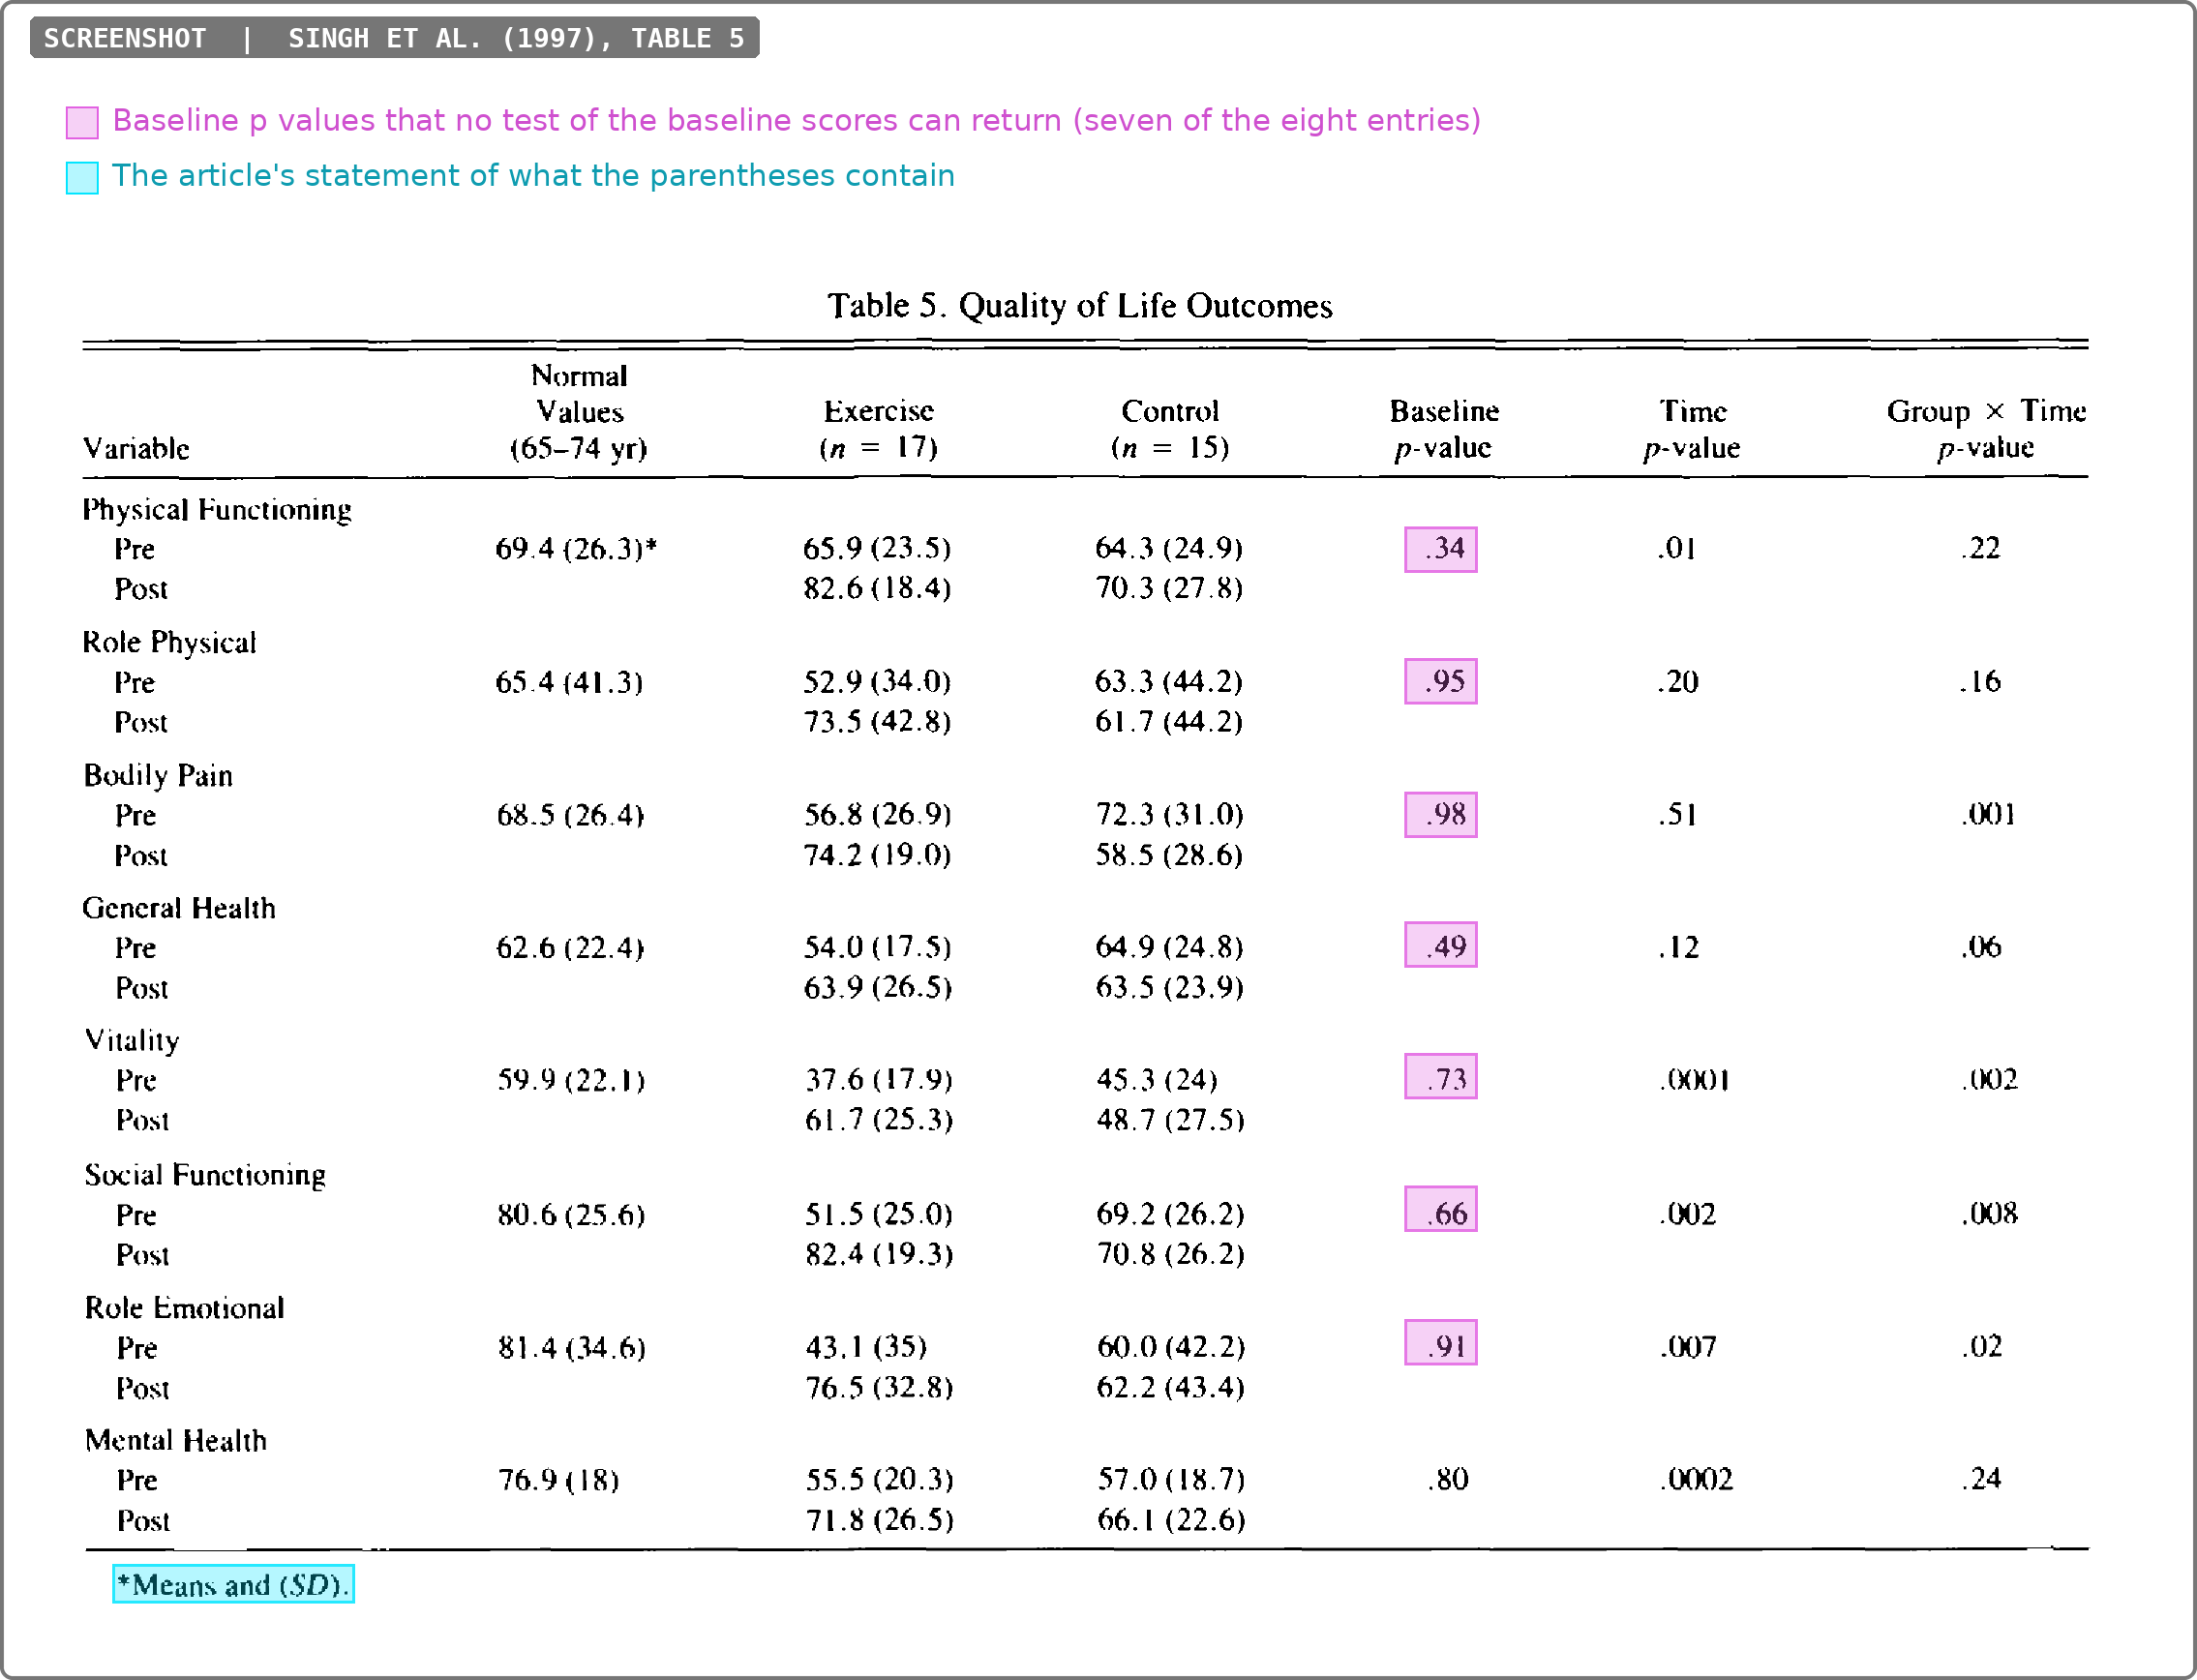
\includegraphics[keepaspectratio]{images/singh_table_5_annotated.png}}

}

\caption{\label{fig-table-5}Table 5 of Singh
(\citeproc{ref-singh1997}{1997}), quality of life outcomes on the SF-36.
Pink marks the 7 ``Baseline p-value'' entries that no test of the
baseline scores can return. Blue marks the footnote. This is the one
table whose parenthetical values the Methods identify as standard
deviations.}

\end{figure}%

We recalculated an unpaired \emph{t} test on the baseline scores of each
of the 8 SF-36 subscales from the reported means, SDs, and sample sizes
(see \hyperref[tbl-baseline]{Table~\ref*{tbl-baseline}}). With every
reported mean and SD free to sit anywhere within its rounding interval,
7 of the 8 reported \emph{p} values fall outside the range that either
\emph{t} test can return, each by more than 0.2. The exception is mental
health, where the groups start and end close together. Reading the SDs
as SEs does not reproduce any of the 8. For bodily pain, the baseline
means of 56.8 and 72.3 with SDs of about 30 give .14, against a reported
\emph{p} value of .98. For social functioning, the baseline means of
51.5 and 69.2 give .06, against a reported .66. For role emotional, the
baseline means of 43.1 and 60.0 give .23, against a reported .91.

The mislabel matters most where a baseline comparison matters. For
bodily pain, social functioning, and role emotional, the groups start 15
to 18 points apart and end close together. A reader of Table 5 would
take the reported values of .98, .66, and .91 to mean that the groups
started out alike.

\begin{figure}[H]

\centering{

\pandocbounded{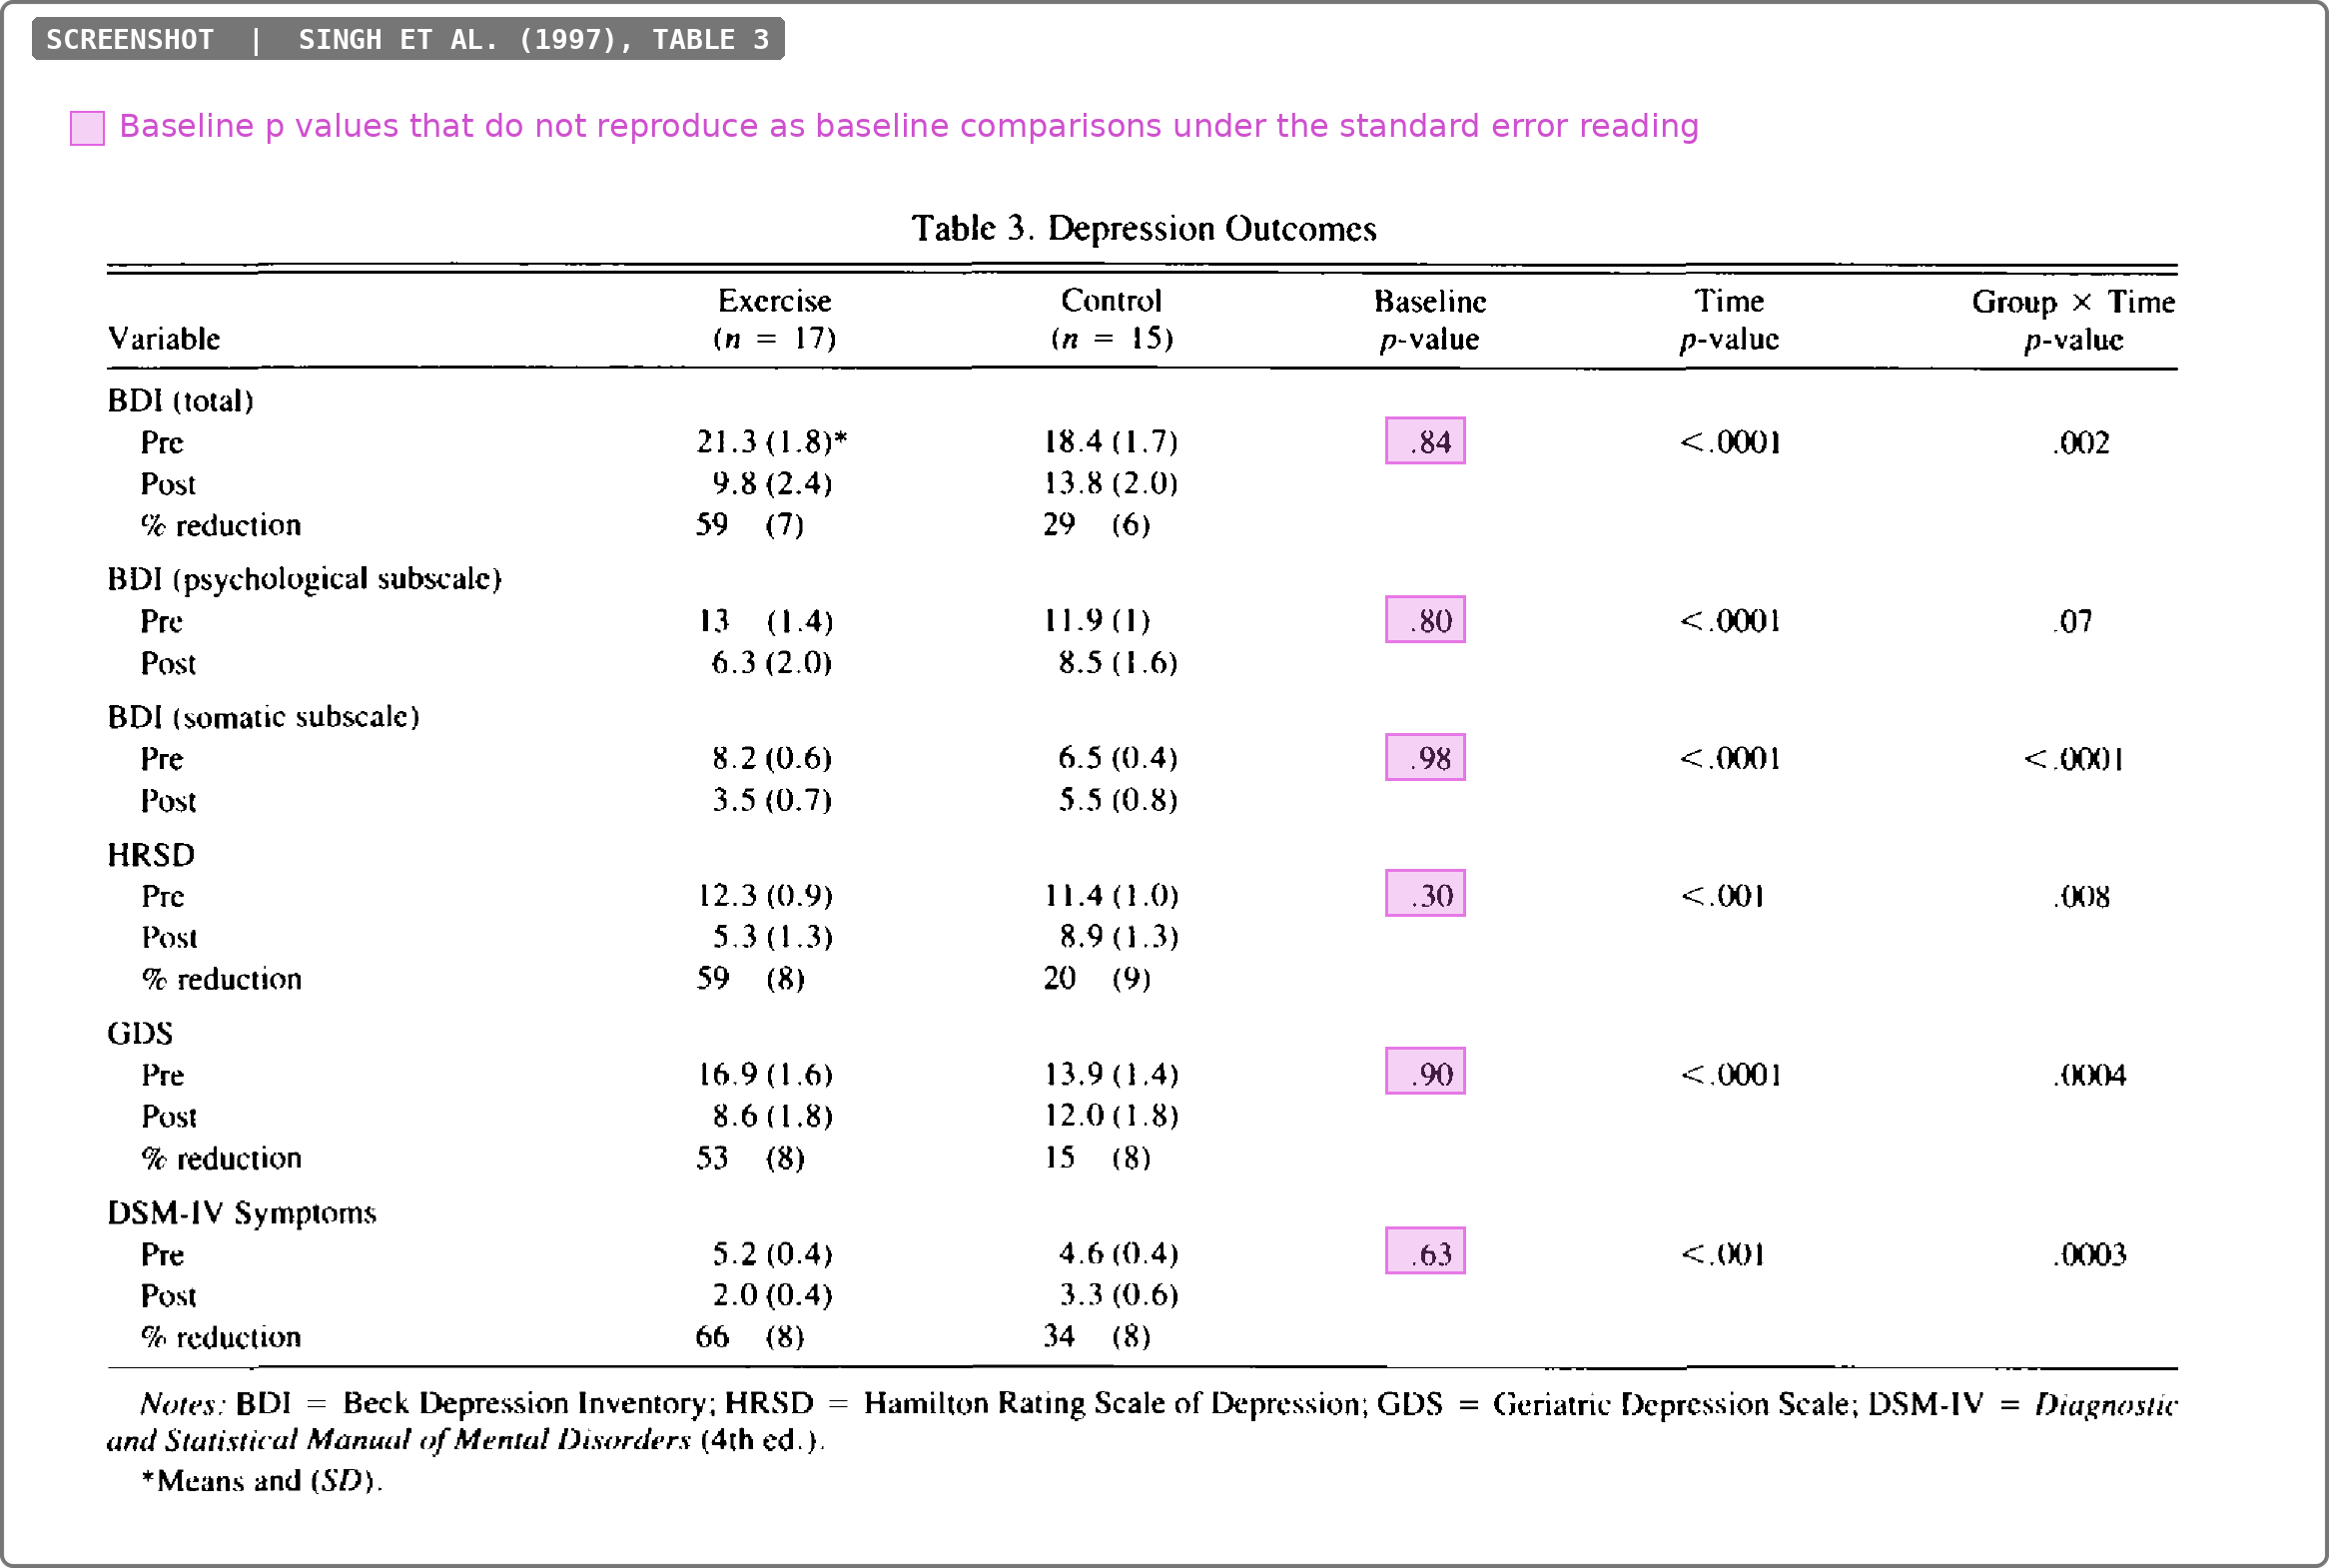
\includegraphics[keepaspectratio]{images/singh_table_3_baseline_annotated.png}}

}

\caption{\label{fig-table-3-baseline}Table 3 of Singh
(\citeproc{ref-singh1997}{1997}). Pink marks the six ``Baseline
p-value'' entries, none of which reproduce as a comparison of the
baseline scores.}

\end{figure}%

The same column appears in the depression outcomes in Table 3 (see
\hyperref[fig-table-3-baseline]{Figure~\ref*{fig-table-3-baseline}}). We
recalculated the baseline \emph{t} test for each of its six measures,
treating the values in parentheses as SEs (see
\hyperref[sec-se-sd]{Section~\ref*{sec-se-sd}} and
\hyperref[tbl-baseline]{Table~\ref*{tbl-baseline}}). None of the six
reported \emph{p} values can be reproduced under either reading of the
parentheticals. One of these discrepancies changes the article's account
of the trial. On the somatic subscale of the BDI, the exercise group
started at 8.2 and the control group at 6.5, with SEs of 0.6 and 0.4.
The baseline \emph{t} test returns a \emph{p} value of .029 (.026 with
Welch's test), against .98 in Table 3. The Results state that ``there
were no significant differences at baseline in any variables measured.''
The somatic subscale is also the outcome with the strongest reported
interaction (\(p < .0001\)), on which the group with the higher baseline
score improved the most. A group that starts with more symptoms has more
room to improve, so a baseline difference on this subscale bears on the
strongest result in the article.

\begin{table}

\caption{\label{tbl-baseline}The Baseline p-value column of Tables 5 and
3 against a test of the baseline scores. Table 5 is read as the Methods
describe it (standard deviations), Table 3 as standard errors.}

\centering{

\centering
\begin{talltblr}[         %% tabularray outer open
entry=none,label=none,
note{}={\textit{Note.} Baseline means and parenthetical values as reported, exercise (n = 17) and control (n = 15). Student is Student's two-sample t test (pooled variance) and Welch is Welch's two-sample t test (unequal variances), each applied to the baseline scores. Each gives the lowest and highest p-value the test can return once every reported value is allowed to sit anywhere in its rounding interval, rounded outward to the reported precision. Reproduces is Yes when the reported value falls inside either range.},
]                     %% tabularray outer close
{                     %% tabularray inner open
colspec={Q[]Q[]Q[]Q[]Q[]Q[]Q[]},
cell{1,4-11,13-18}{1}={}{font=\fontsize{0.9em}{1.2em}\selectfont,},
cell{1,4-11,13-18}{2}={}{halign=c, font=\fontsize{0.9em}{1.2em}\selectfont,},
cell{1,4-11,13-18}{3}={}{halign=c, font=\fontsize{0.9em}{1.2em}\selectfont,},
cell{1,4-11,13-18}{4}={}{halign=c, font=\fontsize{0.9em}{1.2em}\selectfont,},
cell{1,4-11,13-18}{6}={}{halign=c, font=\fontsize{0.9em}{1.2em}\selectfont,},
cell{1}{5}={c=2,}{halign=c, font=\fontsize{0.9em}{1.2em}\selectfont, halign=c,},
cell{1}{7}={}{halign=c, font=\fontsize{0.9em}{1.2em}\selectfont,},
cell{11}{7}={}{halign=c, font=\fontsize{0.9em}{1.2em}\selectfont, fg=c0e9cb0,},
cell{2}{1}={}{font=\fontsize{0.9em}{1.2em}\selectfont, font=\ttfamily, fg=c767676, font=\fontsize{0.85em}{1.15em}\selectfont, font=\ttfamily, fg=c767676, font=\fontsize{0.85em}{1.15em}\selectfont,},
cell{2}{2}={}{halign=c, font=\fontsize{0.9em}{1.2em}\selectfont, font=\ttfamily, fg=c767676, font=\fontsize{0.85em}{1.15em}\selectfont, font=\ttfamily, fg=c767676, font=\fontsize{0.85em}{1.15em}\selectfont,},
cell{2}{3}={}{halign=c, font=\fontsize{0.9em}{1.2em}\selectfont, font=\ttfamily, fg=c767676, font=\fontsize{0.85em}{1.15em}\selectfont, font=\ttfamily, fg=c767676, font=\fontsize{0.85em}{1.15em}\selectfont,},
cell{2}{4}={}{halign=c, font=\fontsize{0.9em}{1.2em}\selectfont, font=\ttfamily, fg=c767676, font=\fontsize{0.85em}{1.15em}\selectfont, font=\ttfamily, fg=c767676, font=\fontsize{0.85em}{1.15em}\selectfont,},
cell{2}{5}={}{halign=c, font=\fontsize{0.9em}{1.2em}\selectfont, font=\ttfamily, fg=c767676, font=\fontsize{0.85em}{1.15em}\selectfont, font=\ttfamily, fg=c767676, font=\fontsize{0.85em}{1.15em}\selectfont,},
cell{2}{6}={}{halign=c, font=\fontsize{0.9em}{1.2em}\selectfont, font=\ttfamily, fg=c767676, font=\fontsize{0.85em}{1.15em}\selectfont, font=\ttfamily, fg=c767676, font=\fontsize{0.85em}{1.15em}\selectfont,},
cell{2}{7}={}{halign=c, font=\fontsize{0.9em}{1.2em}\selectfont, font=\ttfamily, fg=c767676, font=\fontsize{0.85em}{1.15em}\selectfont, font=\ttfamily, fg=c767676, font=\fontsize{0.85em}{1.15em}\selectfont,},
cell{3,12}{1}={c=7,}{font=\itshape, font=\fontsize{0.9em}{1.2em}\selectfont,},
cell{3,12}{2}={}{font=\itshape, halign=c, font=\fontsize{0.9em}{1.2em}\selectfont,},
cell{3,12}{3}={}{font=\itshape, halign=c, font=\fontsize{0.9em}{1.2em}\selectfont,},
cell{3,12}{4}={}{font=\itshape, halign=c, font=\fontsize{0.9em}{1.2em}\selectfont,},
cell{3,12}{5}={}{font=\itshape, halign=c, font=\fontsize{0.9em}{1.2em}\selectfont,},
cell{3,12}{6}={}{font=\itshape, halign=c, font=\fontsize{0.9em}{1.2em}\selectfont,},
cell{3,12}{7}={}{font=\itshape, halign=c, font=\fontsize{0.9em}{1.2em}\selectfont,},
cell{4-10,13-18}{7}={}{halign=c, font=\fontsize{0.9em}{1.2em}\selectfont, font=\bfseries, fg=ccf50cf, bg=cfbe4fb,},
cell{4-11,13-18}{5}={}{halign=c, font=\fontsize{0.9em}{1.2em}\selectfont,},
}                     %% tabularray inner close
\tinytableDefineColor{c767676}{HTML}{767676}
\tinytableDefineColor{cfbe4fb}{HTML}{fbe4fb}
\tinytableDefineColor{ccf50cf}{HTML}{cf50cf}
\tinytableDefineColor{c0e9cb0}{HTML}{0e9cb0}
\toprule
&  &  &  & Reproduced \textit{p} &  &  \\ \cmidrule[lr]{5-6}
Variable & Exercise & Control & Reported \textit{p} & Student & Welch & Reproduces \\ \midrule %% TinyTableHeader
Table 5, baseline values read as standard deviations &  &  &  &  &  &  \\
Physical functioning & 65.9 (23.5) & 64.3 (24.9) & .34 & .84–.87 & .84–.87 & No \\
Role physical & 52.9 (34) & 63.3 (44.2) & .95 & .45–.47 & .45–.48 & No \\
Bodily pain & 56.8 (26.9) & 72.3 (31) & .98 & .13–.15 & .13–.16 & No \\
General health & 54 (17.5) & 64.9 (24.8) & .49 & .13–.18 & .14–.20 & No \\
Vitality & 37.6 (17.9) & 45.3 (24) & .73 & .29–.33 & .30–.34 & No \\
Social functioning & 51.5 (25) & 69.2 (26.2) & .66 & .05–.07 & .05–.07 & No \\
Role emotional & 43.1 (35) & 60 (42.2) & .91 & .20–.25 & .21–.25 & No \\
Mental health & 55.5 (20.3) & 57 (18.7) & .80 & .76–.90 & .76–.90 & Yes \\
Table 3, baseline values read as standard errors &  &  &  &  &  &  \\
BDI total & 21.3 (1.8) & 18.4 (1.7) & .84 & .22–.29 & .22–.29 & No \\
BDI psychological & 13 (1.4) & 11.9 (1) & .80 & .33–.77 & .32–.77 & No \\
BDI somatic & 8.2 (0.6) & 6.5 (0.4) & .98 & .01–.06 & .01–.06 & No \\
HRSD & 12.3 (0.9) & 11.4 (1) & .30 & .43–.58 & .43–.58 & No \\
GDS & 16.9 (1.6) & 13.9 (1.4) & .90 & .14–.21 & .14–.20 & No \\
DSM-IV symptoms & 5.2 (0.4) & 4.6 (0.4) & .63 & .16–.45 & .16–.44 & No \\
\bottomrule
\end{talltblr}

}

\end{table}%

The column is mislabeled in all five tables. The values in it can not be
recovered as baseline comparisons under any reading of the
parentheticals. Each one that no test of the baseline scores can return
is an instance, 7 in Table 5 and 6 in Table 3, for 13 instances of
\href{https://auditclinicalevidence.org/riv.html#riv-2-2}{\textcolor{acerivblue}{\textbf{Statistical Inconsistencies and Impossible Data Sets (RIV 2.2)}}}.
Tables 4, 6, and 7 contain the same column and are described here but
not counted. The article reports no baseline comparison for any outcome,
although it states that none differed at baseline. For at least one
outcome, the somatic subscale of the BDI, the article's own numbers show
a baseline difference.

\subsection{\texorpdfstring{\emph{p} values that can not be reproduced
under any
reading}{p values that can not be reproduced under any reading}}\label{sec-baseline-cat}

Three of the unpaired comparisons in
\hyperref[tbl-sdse-a]{Table~\ref*{tbl-sdse-a}} reproduce under neither
reading of the parentheticals. For ethanol intake in Table 1, the
reported \emph{p} value is .34, against .02--.07 as SDs and .56--.63 as
SEs. For the duration of depressive symptoms, it is .45, against
.01--.06 and .50--.62. For hospital days in Table 2, it is .40, against
.00--.05 and .41--.60. All three variables are skewed, with SEs close to
the size of the means, which points to a few subjects with large values.
Such variables may have been summarized and tested differently (the
Methods allow for medians and ranges ``as appropriate''). As reported,
they are three instances of
\href{https://auditclinicalevidence.org/riv.html#riv-2-2}{\textcolor{acerivblue}{\textbf{Statistical Inconsistencies and Impossible Data Sets (RIV 2.2)}}}.

Table 1 of Singh (\citeproc{ref-singh1997}{1997}) contains a \emph{p}
value for each of 10 categorical baseline characteristics (see
\hyperref[fig-table-1-categorical]{Figure~\ref*{fig-table-1-categorical}}).
The article states that \emph{p} values for categorical data come from
either a chi-square test or Fisher's exact test, without saying which
variable uses which. The Results identify the test through three
comparisons of proportions reported with their \emph{p} values: response
to treatment in 10/17 exercisers vs 4/15 controls (\(p = .067\)),
remission of minor depression in 6/7 vs 4/10 (\(p = .06\)), and
remission of major depression in 8/9 vs 2/4 (\(p = .12\)). Pearson's
chi-square test without a continuity correction reproduces all three
(.067, .059, and .125, respectively). Fisher's exact test reproduces
none of them (.087, .134, and .203, respectively). The authors therefore
used an uncorrected chi-square test, even for tables with expected cell
counts well below five, where the chi-square approximation is unreliable
and Fisher's exact test is the usual choice.

\begin{figure}[H]

\centering{

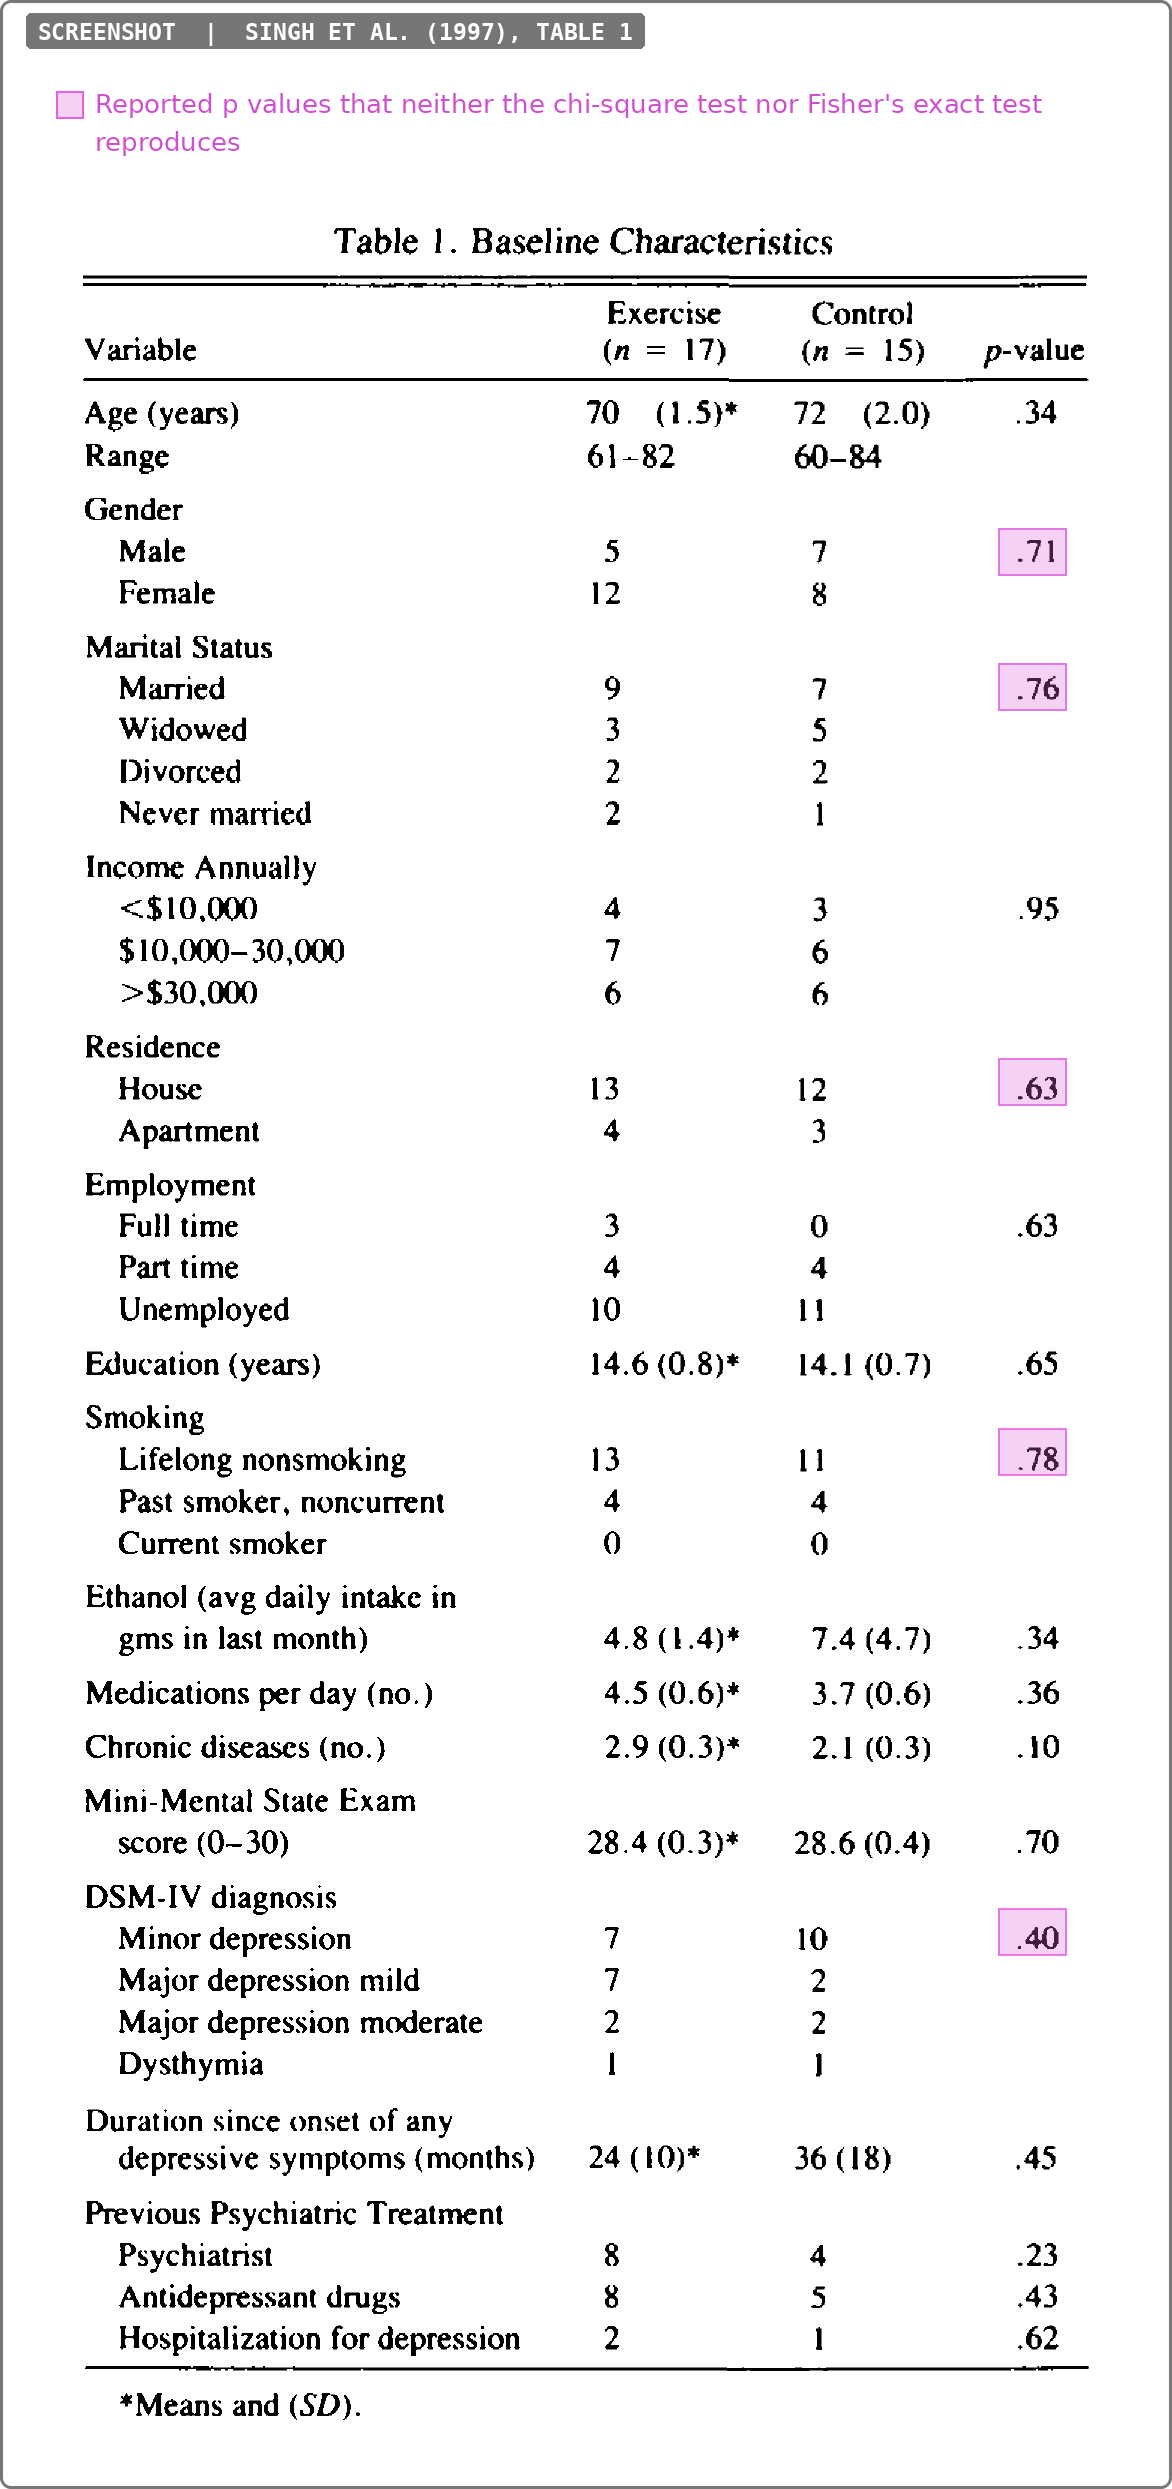
\includegraphics[width=0.62\linewidth,height=\textheight,keepaspectratio]{images/singh_table_1_categorical_annotated.png}

}

\caption{\label{fig-table-1-categorical}Table 1 of Singh
(\citeproc{ref-singh1997}{1997}). Pink marks the five categorical
\emph{p} values that neither the chi-square test nor Fisher's exact test
reproduces from the reported counts.}

\end{figure}%

We recalculated this test, and Fisher's exact test, from the contingency
table cells reported in Table 1 (see
\hyperref[tbl-t1-categorical]{Table~\ref*{tbl-t1-categorical}}). Four of
the 10 \emph{p} values reproduce under the uncorrected chi-square test,
those for annual income, previous treatment by a psychiatrist, previous
antidepressant drugs, and previous hospitalization. Neither test
reproduces the other six. For gender (5 men and 12 women vs 7 men and 8
women), the two tests return .31 and .47 against a reported \emph{p}
value of .71. For residence (13 house and 4 apartment vs 12 and 3), they
return .81 and 1.00 against a reported .63. Two variants of the
chi-square test, the Yates continuity correction and the likelihood
ratio test, do not change this. None of the six 2 by 2 tables returns
its reported value under the Yates corrected chi-square test. The
likelihood ratio test agrees with the uncorrected chi-square test to the
reported precision. Before counting a \emph{p} value as irreproducible,
we also tried every way of collapsing the categories of each variable
into fewer groups, under all four tests. This collapsing reproduces one
variable, employment. Collapsing full-time and part-time work into a
single employed category and applying the Yates correction returns .625,
which rounds to the reported value. The article describes no such
collapsing and uses a continuity correction nowhere else. No collapsing
of the marital status or DSM-IV diagnosis categories reproduces the
reported \emph{p} values under any of the four tests.

\begin{table}

\caption{\label{tbl-t1-categorical}Baseline p-values for the categorical
characteristics in Table 1, reproduced from the reported counts.}

\centering{

\centering
\begin{talltblr}[         %% tabularray outer open
entry=none,label=none,
note{}={\textit{Note.} Counts as reported in Table 1 of the article. Roman numerals are the levels of each characteristic in the article's row order: gender, I male, II female; marital status, I married, II widowed, III divorced, IV never married; income, I below \$10,000, II \$10,000 to \$30,000, III above \$30,000; residence, I house, II apartment; employment, I full time, II part time, III unemployed; smoking, I lifelong nonsmoker, II past smoker (the empty current smoker row is omitted); DSM-IV diagnosis, I minor depression, II major depression mild, III major depression moderate, IV dysthymia; previous psychiatrist, antidepressant drugs, and hospitalization, I yes, II no (the article reports the yes counts). Chi-squared is Pearson's test without a continuity correction, the test that reproduces the article's own comparisons of proportions in the Results; Fisher is the Fisher-Freeman-Halton exact test for tables larger than 2 by 2. None of the six 2 by 2 tables returns its reported value under the Yates corrected chi-square test either. Reproduces means that at least one test returns the reported value to within a unit in the last digit.},
]                     %% tabularray outer close
{                     %% tabularray inner open
colspec={Q[]Q[]Q[]Q[]Q[]Q[]Q[]Q[]Q[]Q[]Q[]Q[]Q[]},
cell{1,3-12}{1}={}{font=\fontsize{0.9em}{1.2em}\selectfont,},
cell{1,3-12}{10}={}{halign=c, font=\fontsize{0.9em}{1.2em}\selectfont,},
cell{1,3-12}{12}={}{halign=c, font=\fontsize{0.9em}{1.2em}\selectfont,},
cell{1,3-12}{3}={}{halign=c, font=\fontsize{0.9em}{1.2em}\selectfont,},
cell{1,3-12}{4}={}{halign=c, font=\fontsize{0.9em}{1.2em}\selectfont,},
cell{1,3-12}{5}={}{halign=c, font=\fontsize{0.9em}{1.2em}\selectfont,},
cell{1,3-12}{7}={}{halign=c, font=\fontsize{0.9em}{1.2em}\selectfont,},
cell{1,3-12}{8}={}{halign=c, font=\fontsize{0.9em}{1.2em}\selectfont,},
cell{1,3-12}{9}={}{halign=c, font=\fontsize{0.9em}{1.2em}\selectfont,},
cell{1}{11}={c=2,}{halign=c, font=\fontsize{0.9em}{1.2em}\selectfont, halign=c,},
cell{1}{13}={}{halign=c, font=\fontsize{0.9em}{1.2em}\selectfont,},
cell{1}{2}={c=4,}{halign=c, font=\fontsize{0.9em}{1.2em}\selectfont, halign=c,},
cell{1}{6}={c=4,}{halign=c, font=\fontsize{0.9em}{1.2em}\selectfont, halign=c,},
cell{2}{1}={}{font=\fontsize{0.9em}{1.2em}\selectfont, font=\ttfamily, fg=c767676, font=\fontsize{0.85em}{1.15em}\selectfont,},
cell{2}{10}={}{halign=c, font=\fontsize{0.9em}{1.2em}\selectfont, font=\ttfamily, fg=c767676, font=\fontsize{0.85em}{1.15em}\selectfont,},
cell{2}{11}={}{halign=c, font=\fontsize{0.9em}{1.2em}\selectfont, font=\ttfamily, fg=c767676, font=\fontsize{0.85em}{1.15em}\selectfont,},
cell{2}{12}={}{halign=c, font=\fontsize{0.9em}{1.2em}\selectfont, font=\ttfamily, fg=c767676, font=\fontsize{0.85em}{1.15em}\selectfont,},
cell{2}{13}={}{halign=c, font=\fontsize{0.9em}{1.2em}\selectfont, font=\ttfamily, fg=c767676, font=\fontsize{0.85em}{1.15em}\selectfont,},
cell{2}{2}={}{halign=c, font=\fontsize{0.9em}{1.2em}\selectfont, font=\ttfamily, fg=c767676, font=\fontsize{0.85em}{1.15em}\selectfont,},
cell{2}{3}={}{halign=c, font=\fontsize{0.9em}{1.2em}\selectfont, font=\ttfamily, fg=c767676, font=\fontsize{0.85em}{1.15em}\selectfont,},
cell{2}{4}={}{halign=c, font=\fontsize{0.9em}{1.2em}\selectfont, font=\ttfamily, fg=c767676, font=\fontsize{0.85em}{1.15em}\selectfont,},
cell{2}{5}={}{halign=c, font=\fontsize{0.9em}{1.2em}\selectfont, font=\ttfamily, fg=c767676, font=\fontsize{0.85em}{1.15em}\selectfont,},
cell{2}{6}={}{halign=c, font=\fontsize{0.9em}{1.2em}\selectfont, font=\ttfamily, fg=c767676, font=\fontsize{0.85em}{1.15em}\selectfont,},
cell{2}{7}={}{halign=c, font=\fontsize{0.9em}{1.2em}\selectfont, font=\ttfamily, fg=c767676, font=\fontsize{0.85em}{1.15em}\selectfont,},
cell{2}{8}={}{halign=c, font=\fontsize{0.9em}{1.2em}\selectfont, font=\ttfamily, fg=c767676, font=\fontsize{0.85em}{1.15em}\selectfont,},
cell{2}{9}={}{halign=c, font=\fontsize{0.9em}{1.2em}\selectfont, font=\ttfamily, fg=c767676, font=\fontsize{0.85em}{1.15em}\selectfont,},
cell{3-12}{11}={}{halign=c, font=\fontsize{0.9em}{1.2em}\selectfont,},
cell{3-12}{2}={}{halign=c, font=\fontsize{0.9em}{1.2em}\selectfont,},
cell{3-12}{6}={}{halign=c, font=\fontsize{0.9em}{1.2em}\selectfont,},
cell{3-4,6-9}{13}={}{halign=c, font=\fontsize{0.9em}{1.2em}\selectfont, font=\bfseries, fg=ccf50cf, bg=cfbe4fb,},
cell{5,10-12}{13}={}{halign=c, font=\fontsize{0.9em}{1.2em}\selectfont, fg=c0e9cb0,},
}                     %% tabularray inner close
\tinytableDefineColor{c767676}{HTML}{767676}
\tinytableDefineColor{cfbe4fb}{HTML}{fbe4fb}
\tinytableDefineColor{ccf50cf}{HTML}{cf50cf}
\tinytableDefineColor{c0e9cb0}{HTML}{0e9cb0}
\toprule
& Exercise (n = 17) &  &  &  & Control (n = 15) &  &  &  &  & Reproduced \textit{p} &  &  \\ \cmidrule[lr]{2-5}\cmidrule[lr]{6-9}\cmidrule[lr]{11-12}
Characteristic & I & II & III & IV & I  & II  & III  & IV  & Reported \textit{p} & Chi-squared & Fisher & Reproduces \\ \midrule %% TinyTableHeader
Gender & 5 & 12 & - & - & 7 & 8 & - & - & .71 & .31 & .47 & No \\
Marital status & 9 & 3 & 2 & 2 & 7 & 5 & 2 & 1 & .76 & .79 & .85 & No \\
Income & 4 & 7 & 6 & - & 3 & 6 & 6 & - & .95 & .95 & 1.00 & Yes \\
Residence & 13 & 4 & - & - & 12 & 3 & - & - & .63 & .81 & 1.00 & No \\
Employment & 3 & 4 & 10 & - & 0 & 4 & 11 & - & .63 & .23 & .35 & No \\
Smoking & 13 & 4 & - & - & 11 & 4 & - & - & .78 & .84 & 1.00 & No \\
DSM-IV diagnosis & 7 & 7 & 2 & 1 & 10 & 2 & 2 & 1 & .40 & .36 & .32 & No \\
Psychiatrist & 8 & 9 & - & - & 4 & 11 & - & - & .23 & .23 & .29 & Yes \\
Antidepressant drugs & 8 & 9 & - & - & 5 & 10 & - & - & .43 & .43 & .49 & Yes \\
Hospitalization & 2 & 15 & - & - & 1 & 14 & - & - & .62 & .62 & 1.00 & Yes \\
\bottomrule
\end{talltblr}

}

\end{table}%

The irreproducible categorical \emph{p} values do not affect the
conclusions of the study. The reported and recalculated values are all
above .05, so under either set the groups do not differ significantly on
these characteristics. We count them because they are incorrect. A
baseline table that does not reproduce from its own contingency table
cells also limits how far a reader can verify the article's other
computations. The five \emph{p} values that no test reproduces, from the
reported cells or from any collapsing of them, are five instances of
\href{https://auditclinicalevidence.org/riv.html#riv-2-2}{\textcolor{acerivblue}{\textbf{Statistical Inconsistencies and Impossible Data Sets (RIV 2.2)}}}.
Employment is described but not counted.

\subsection{Training intensity SDs that their ranges do not
allow}\label{sec-intensity}

The Results report the mean training intensity of the exercise group as
``78\% (\emph{SD} = 24) of the 1RM (range 45--87\%)''. Excluding the one
subject who had less than 50\% compliance, they report ``80\% (\emph{SD}
= 10) of the 1RM (range 70--87\%)''. Both values are labeled SD in the
text (the 1RM is the one-repetition maximum, the heaviest weight a
subject can lift once, so intensity is the training load as a percentage
of it). A set of \(n\) values that lies within a range of width \(w\)
has an SD of at most \(\tfrac{w}{2}\sqrt{n/(n-1)}\), reached when half
of the values sit at each end. For the 17 exercisers between 45\% and
87\%, the SD can be at most 22.2, even with each end of the range
rounded outward by half a point. For the 16 exercisers between 70\% and
87\%, it can be at most 9.3. Neither reported SD is possible. Read as
SEs, the implied SDs of 99 and 40 are larger still. No reading of these
values is possible, so they are two instances of
\href{https://auditclinicalevidence.org/riv.html#riv-2-2}{\textcolor{acerivblue}{\textbf{Statistical Inconsistencies and Impossible Data Sets (RIV 2.2)}}}.
The Discussion repeats the first value (``mean 78, \emph{SD} = 24''),
which is described but not counted.

\subsection{GRIM failure in a subgroup mean}\label{sec-grim}

The \emph{granularity-related inconsistency of means} test (GRIM,
\citeproc{ref-grim}{Brown 2017}) checks whether a reported mean can
arise from integer scores, given the sample size. The BDI and HRSD are
sums of integer item scores, so a group mean must be an integer divided
by the group size. A mean reported to one decimal place can only fail
the test when the group has fewer than 10 subjects. Of the 12 such means
in Table 4, one fails. The baseline HRSD mean of 13.6 for the four
control subjects with major depression would require an integer total
between 54.2 and 54.6. No integer lies in that range (see
\hyperref[fig-table-4-grim]{Figure~\ref*{fig-table-4-grim}}). The
nearest achievable means are 13.5 and 13.75. The other 11 means are
consistent.

\begin{figure}[H]

\centering{

\pandocbounded{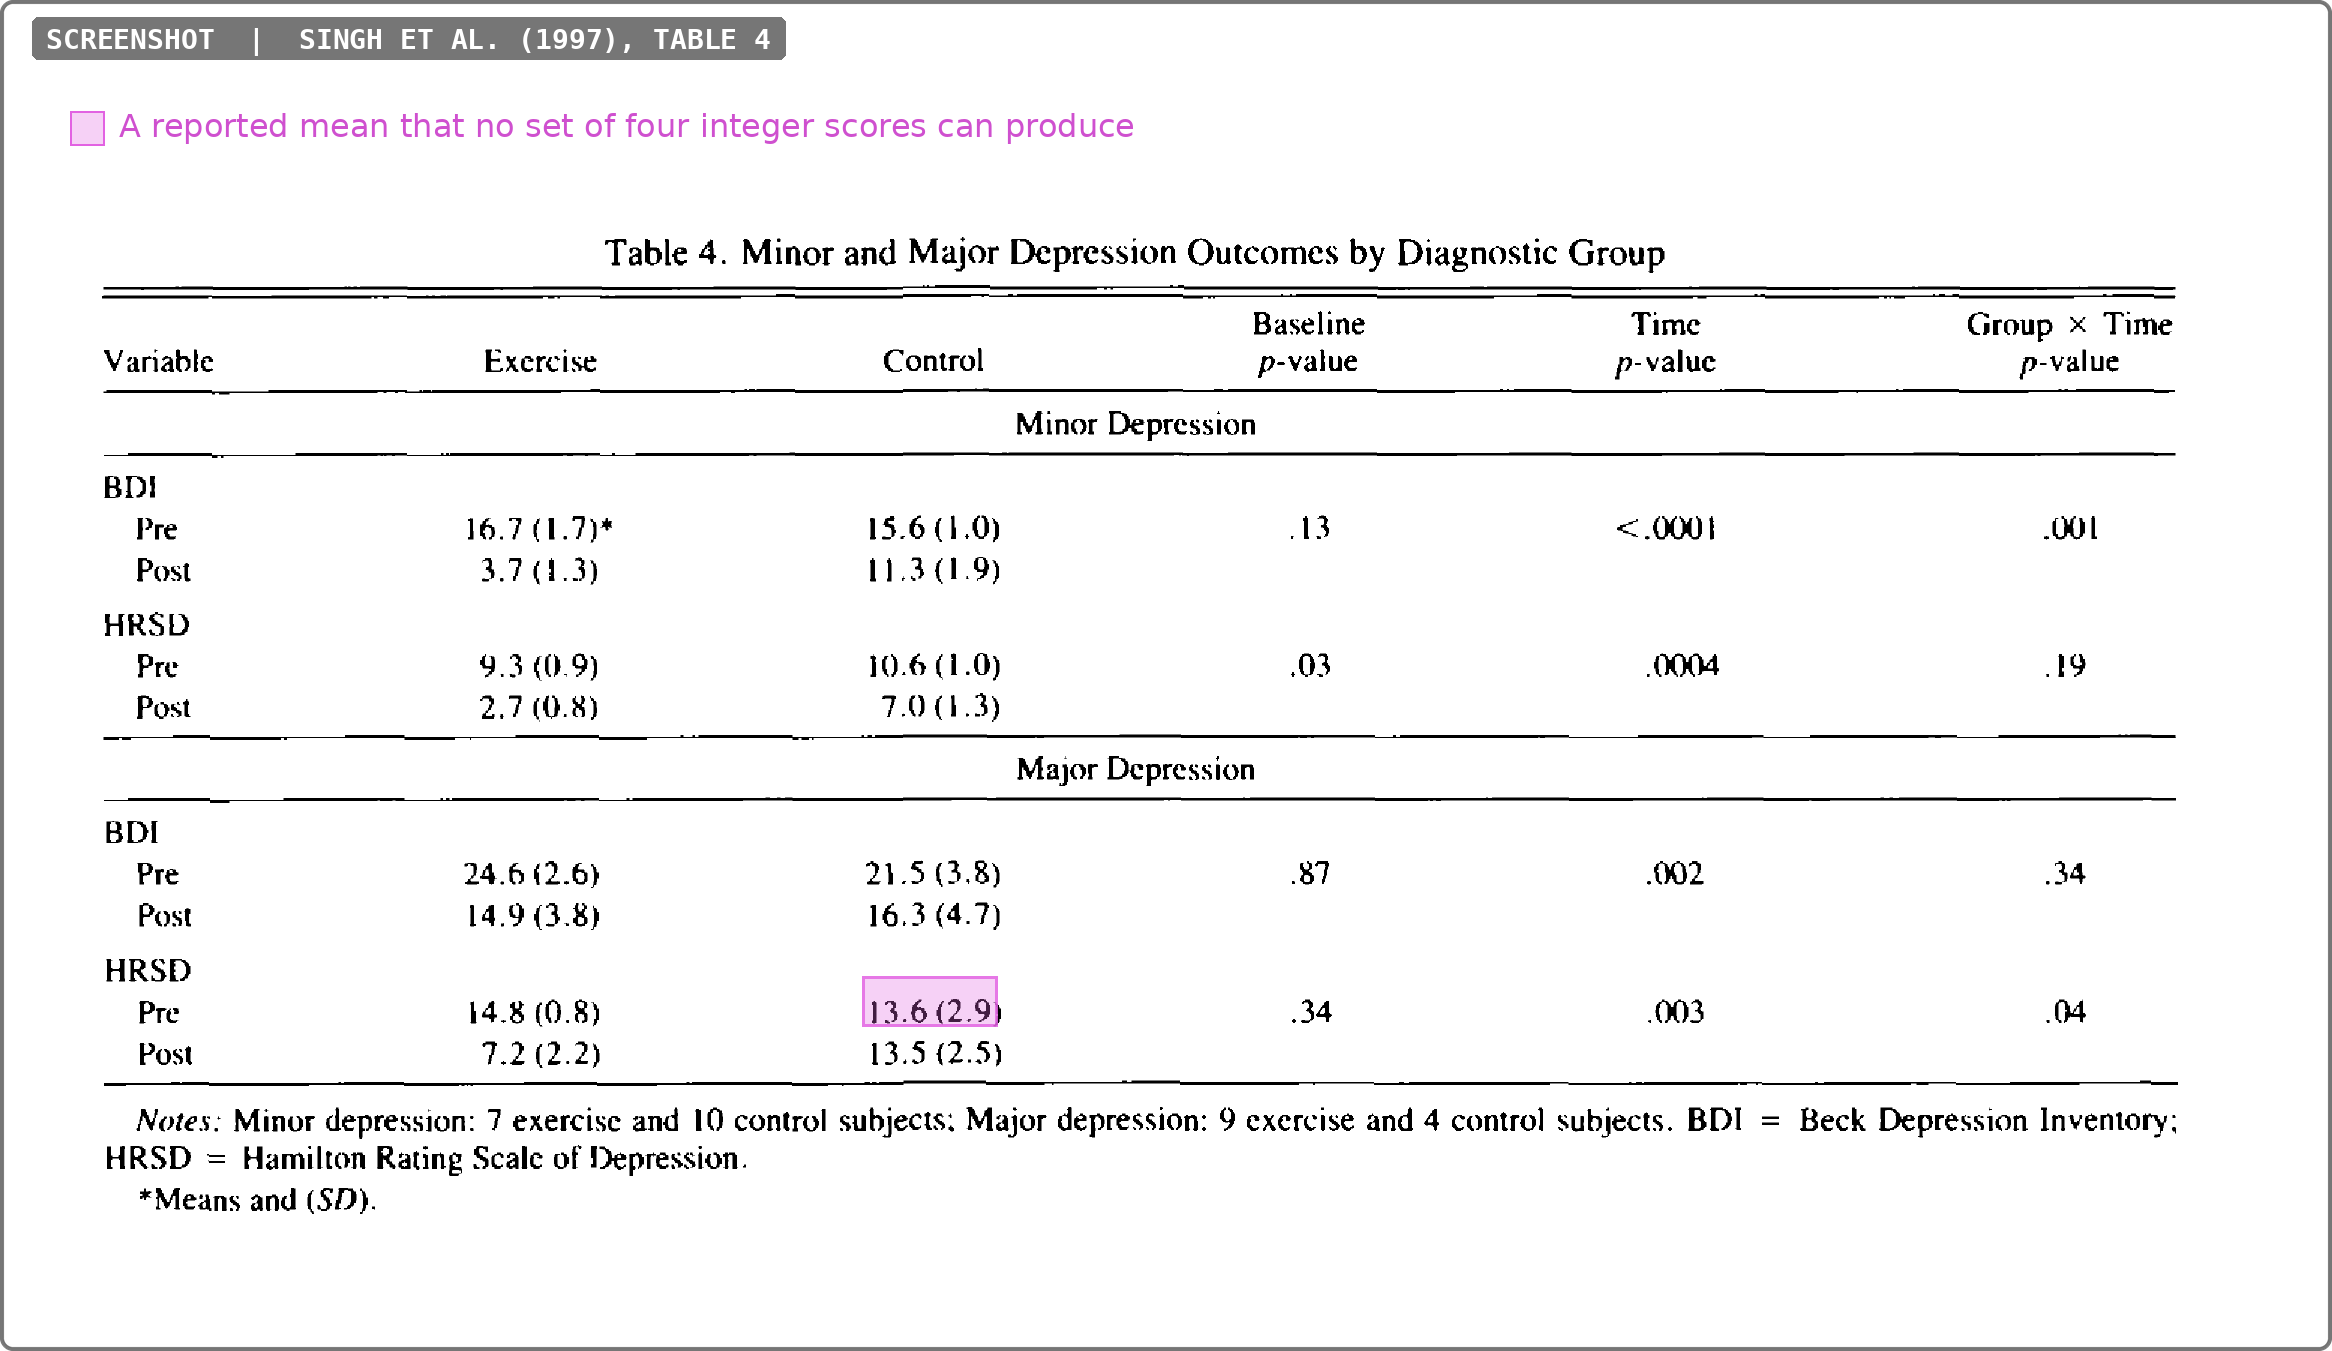
\includegraphics[keepaspectratio]{images/singh_table_4_grim_annotated.png}}

}

\caption{\label{fig-table-4-grim}Table 4 of Singh
(\citeproc{ref-singh1997}{1997}). Pink marks the baseline HRSD mean of
the four control subjects with major depression, which no set of four
integer scores can produce.}

\end{figure}%

Rounding, the scale, and the sample size do not explain the failure. The
notes to Table 4 give the subgroup size as 4, which matches the DSM-IV
diagnosis counts in Table 1 (2 mild and 2 moderate major depression).
The HRSD is scored in whole points. The test already allows for
rounding. The Results state that the improvement in HRSD scores in this
subgroup was twice that of controls, a comparison that depends on the
impossible mean. This is one instance of
\href{https://auditclinicalevidence.org/riv.html#riv-2-2}{\textcolor{acerivblue}{\textbf{Statistical Inconsistencies and Impossible Data Sets (RIV 2.2)}}}.

The other values in the article that can be checked are consistent. The
three correlations reported in the Results for the exercise group
(\(r =\) −0.786, −0.589, and 0.500 with \(n = 17\)) give \emph{p} values
of .0002, .013, and .04, against reported values of .0002, .013, and
.04. The diagnostic subgroup sizes sum to the group sizes once the
dysthymic subject in each group is included. The available evidence
points to problems in how the statistics are labeled and reported. It
gives no reason to doubt that the trial took place.

\section{Conclusion}\label{sec-conclusion}

The audited article describes a small RCT whose tables misstate what
they contain. Every table of continuous outcomes labels the values in
parentheses as standard deviations, yet the Methods state that they are
standard errors. The reported test statistics support the Methods (i.e.,
the values in parentheses are standard errors). For 25 variables across
Tables 1 through 4, 6, and 7, the reported \emph{p} value can not be
reproduced with the values read as SDs and can be with the values read
as SEs. Additionally, the reported age ranges and the Table 4 subgroup
means are impossible under the labeled SDs. This warrants 86 instances
of
\href{https://auditclinicalevidence.org/riv.html#riv-2-4}{\textcolor{acerivblue}{\textbf{Data Miscalculation or Erroneous Reporting (RIV 2.4)}}},
one for each of the values involved.

The effect of this error on meta-analyses is the central finding of this
report. The largest post-test SMD the article can support is −0.72
(−0.44 for the BDI). Of the 24 meta-analyses we located that report an
effect size for this trial, 19 assign Singh
(\citeproc{ref-singh1997}{1997}) a value beyond anything a correct
extraction can produce. The median assigned value is −2.74. In two
syntheses this 32-subject trial is the largest effect in the analysis by
a factor of two or more. Four meta-analyses, including the Cochrane
review, report exactly −1.75, the value that results from meta-analysts
treating the standard errors of the post-intervention BDI scores as
standard deviations. For nearly 30 years, the evidence base on exercise
and depression has carried a moderate effect as one of its largest.

The columns labeled ``Baseline \emph{p}-value'' in the outcome tables do
not report baseline comparisons. In the one table where the SDs are
unambiguous, 7 of the 8 reported \emph{p} values can not be reproduced
as a test of the baseline scores. Under the correct reading of the
depression outcomes, the groups differed at baseline on the somatic
subscale of the BDI, the outcome with the strongest reported
interaction. Yet the Results state that no variable differed at
baseline. The 13 reported values that no baseline test can return are 13
instances of
\href{https://auditclinicalevidence.org/riv.html#riv-2-2}{\textcolor{acerivblue}{\textbf{Statistical Inconsistencies and Impossible Data Sets (RIV 2.2)}}}.
Furthermore, three unpaired and five categorical \emph{p} values in
Tables 1 and 2 can not be reproduced under any reading of the reported
summaries, which adds 8 instances of
\href{https://auditclinicalevidence.org/riv.html#riv-2-2}{\textcolor{acerivblue}{\textbf{Statistical Inconsistencies and Impossible Data Sets (RIV 2.2)}}}.
Two training intensity SDs in the Results are larger than their ranges
allow under either reading, which adds two more. One subgroup mean in
Table 4 is impossible given its sample size, which adds one.

Because the misreporting in Singh (\citeproc{ref-singh1997}{1997}) has
contaminated the evidence syntheses in this field, we recommend
\emph{retraction}. Every table labels the standard errors as standard
deviations. Of the 24 meta-analyses we located, 19 assign Singh
(\citeproc{ref-singh1997}{1997}) an effect size that no correct
extraction can produce. Four of these meta-analyses, including the
Cochrane review, report the value that results from treating the
standard errors as standard deviations. A reader can only use the
published tables as evidence after first correcting them. For nearly 30
years, most meta-analysts have not. In addition, the outcome tables
report \emph{p} values under the label of a baseline comparison that no
test of the baseline scores can return. Furthermore, 8 \emph{p} values
in Tables 1 and 2 can not be reproduced under any reading. One subgroup
mean in Table 4 is impossible given its sample size. As published, the
article's results have no evidentiary value. This recommendation does
not rest on any evidence that the trial was not conducted.

The retraction notice should give the reasons. These are that (a) the
values in parentheses in Tables 1 through 4, 6, and 7 and in the
abstract are standard errors, (b) the first \emph{p} value column of
Tables 3 through 7 does not report a comparison of the groups at
baseline, (c) the groups differed at baseline on the somatic subscale of
the BDI, (d) 8 \emph{p} values in Tables 1 and 2 can not be reproduced
from the reported summaries, (e) the subgroup mean in Table 4 is
impossible given its sample size, and (f) the two training intensity SDs
in the Results are impossible given their ranges.

Whatever the journal decides, meta-analysts and guideline developers who
have included this trial should check the values they extracted from it.
A meta-analysis that recorded the values in parentheses as standard
deviations has treated a moderate effect as a very large one. Such a
meta-analysis should re-extract the study with those values multiplied
by the square root of the group size, or exclude the study.

% keep the RIV summary table on one page
\needspace{12\baselineskip}

\begin{longtable}[]{@{}
  >{\raggedright\arraybackslash}p{(\linewidth - 6\tabcolsep) * \real{0.1429}}
  >{\raggedright\arraybackslash}p{(\linewidth - 6\tabcolsep) * \real{0.5714}}
  >{\centering\arraybackslash}p{(\linewidth - 6\tabcolsep) * \real{0.1429}}
  >{\centering\arraybackslash}p{(\linewidth - 6\tabcolsep) * \real{0.1429}}@{}}
\caption{Summary of Research Integrity Violations identified in the
audited Singh, Clements, and Fiatarone (1997) trial (ACE-RIV
v1.0)}\label{tbl-riv-summary}\tabularnewline
\toprule\noalign{}
\begin{minipage}[b]{\linewidth}\raggedright
{\aceTableHead RIV}
\end{minipage} & \begin{minipage}[b]{\linewidth}\raggedright
{\aceTableHead Title}
\end{minipage} & \begin{minipage}[b]{\linewidth}\centering
{\aceTableHead Instances}
\end{minipage} & \begin{minipage}[b]{\linewidth}\centering
{\aceTableHead Section}
\end{minipage} \\
\midrule\noalign{}
\endfirsthead
\toprule\noalign{}
\begin{minipage}[b]{\linewidth}\raggedright
{\aceTableHead RIV}
\end{minipage} & \begin{minipage}[b]{\linewidth}\raggedright
{\aceTableHead Title}
\end{minipage} & \begin{minipage}[b]{\linewidth}\centering
{\aceTableHead Instances}
\end{minipage} & \begin{minipage}[b]{\linewidth}\centering
{\aceTableHead Section}
\end{minipage} \\
\midrule\noalign{}
\endhead
\bottomrule\noalign{}
\endlastfoot
\textbf{RIV 2.2} & Statistical Inconsistencies and Impossible Data Sets
& 24 & \hyperref[sec-baseline-column]{3.A},
\hyperref[sec-baseline-cat]{3.B}, \hyperref[sec-intensity]{3.C},
\hyperref[sec-grim]{3.D} \\
\textbf{RIV 2.4} & Data Miscalculation or Erroneous Reporting & 86 &
\hyperref[sec-sdse]{2.C} \\
\textbf{\emph{Total}} & & \textbf{\emph{110}} & \\
\end{longtable}

\clearpage

\section*{References}\label{references}
\addcontentsline{toc}{section}{References}

\protect\phantomsection\label{refs}
\begin{CSLReferences}{0}{1}
\bibitem[\citeproctext]{ref-singh1997}
Singh, Clements, Fiatarone (1997) A randomized controlled trial of
progressive resistance training in depressed elders. \emph{The Journals
of Gerontology Series A}. DOI:
\href{https://doi.org/10.1093/gerona/52A.1.M27}{10.1093/gerona/52A.1.M27}.

\bibitem[\citeproctext]{ref-gordon2018}
Gordon, McDowell, Hallgren, Meyer, Lyons, Herring (2018) Association of
efficacy of resistance exercise training with depressive symptoms:
Meta-analysis and meta-regression analysis of randomized clinical
trials. \emph{JAMA Psychiatry}. DOI:
\href{https://doi.org/10.1001/jamapsychiatry.2018.0572}{10.1001/jamapsychiatry.2018.0572}.

\bibitem[\citeproctext]{ref-dai2024}
Dai, Ting, Malau, Wu, Lin, Lin, Chen (2024) Motivational barriers and
facilitators for older adults' engagement in exercise during depressive
episodes: A network meta-analysis of randomized controlled trials.
\emph{Healthcare}. DOI:
\href{https://doi.org/10.3390/healthcare12151498}{10.3390/healthcare12151498}.

\bibitem[\citeproctext]{ref-li2026}
Li, Chen, He, Yan, Zhang, Li (2026) Can exercise truly alleviate
mild-to-moderate and subthreshold depression? Evidence from randomized
controlled trials. \emph{Frontiers in Psychology}. DOI:
\href{https://doi.org/10.3389/fpsyg.2026.1815160}{10.3389/fpsyg.2026.1815160}.

\bibitem[\citeproctext]{ref-lawlor2001}
Lawlor, Hopker (2001) The effectiveness of exercise as an intervention
in the management of depression: Systematic review and meta-regression
analysis of randomised controlled trials. \emph{BMJ}. DOI:
\href{https://doi.org/10.1136/bmj.322.7289.763}{10.1136/bmj.322.7289.763}.

\bibitem[\citeproctext]{ref-liu2011}
Liu, Latham (2011) Can progressive resistance strength training reduce
physical disability in older adults? A meta-analysis study.
\emph{Disability and Rehabilitation}. DOI:
\href{https://doi.org/10.3109/09638288.2010.487145}{10.3109/09638288.2010.487145}.

\bibitem[\citeproctext]{ref-yu2022}
Yu, Wong, Lei, Nie, Shi, Zou, Kong (2022) Comparative effectiveness of
multiple exercise interventions in the treatment of mental health
disorders: A systematic review and network meta-analysis. \emph{Sports
Medicine - Open}. DOI:
\href{https://doi.org/10.1186/s40798-022-00529-5}{10.1186/s40798-022-00529-5}.

\bibitem[\citeproctext]{ref-cooney2013}
Cooney, Dwan, Greig, Lawlor, Rimer, Waugh, McMurdo, Mead (2013) Exercise
for depression. \emph{Cochrane Database of Systematic Reviews}. DOI:
\href{https://doi.org/10.1002/14651858.CD004366.pub6}{10.1002/14651858.CD004366.pub6}.

\bibitem[\citeproctext]{ref-heinzel2015}
Heinzel, Lawrence, Kallies, Rapp, Heissel (2015) Using exercise to fight
depression in older adults: A systematic review and meta-analysis.
\emph{GeroPsych}. DOI:
\href{https://doi.org/10.1024/1662-9647/a000133}{10.1024/1662-9647/a000133}.

\bibitem[\citeproctext]{ref-rhyner2016}
Rhyner, Watts (2016) Exercise and depressive symptoms in older adults: A
systematic meta-analytic review. \emph{Journal of Aging and Physical
Activity}. DOI:
\href{https://doi.org/10.1123/japa.2015-0146}{10.1123/japa.2015-0146}.

\bibitem[\citeproctext]{ref-kvam2016}
Kvam, Kleppe, Nordhus, Hovland (2016) Exercise as a treatment for
depression: A meta-analysis. \emph{Journal of Affective Disorders}. DOI:
\href{https://doi.org/10.1016/j.jad.2016.03.063}{10.1016/j.jad.2016.03.063}.

\bibitem[\citeproctext]{ref-krogh2017}
Krogh, Hjorthøj, Speyer, Gluud, Nordentoft (2017) Exercise for patients
with major depression: A systematic review with meta-analysis and trial
sequential analysis. \emph{BMJ Open}. DOI:
\href{https://doi.org/10.1136/bmjopen-2016-014820}{10.1136/bmjopen-2016-014820}.

\bibitem[\citeproctext]{ref-silveira2013}
Silveira, Moraes, Oliveira, Coutinho, Laks, Deslandes (2013) Physical
exercise and clinically depressed patients: A systematic review and
meta-analysis. \emph{Neuropsychobiology}. DOI:
\href{https://doi.org/10.1159/000345160}{10.1159/000345160}.

\bibitem[\citeproctext]{ref-schuch2016a}
Schuch, Vancampfort, Richards, Rosenbaum, Ward, Stubbs (2016a) Exercise
as a treatment for depression: A meta-analysis adjusting for publication
bias. \emph{Journal of Psychiatric Research}. DOI:
\href{https://doi.org/10.1016/j.jpsychires.2016.02.023}{10.1016/j.jpsychires.2016.02.023}.

\bibitem[\citeproctext]{ref-schuch2016b}
Schuch, Vancampfort, Rosenbaum, Richards, Ward, Veronese, Solmi, Cadore,
Stubbs (2016b) Exercise for depression in older adults: A meta-analysis
of randomized controlled trials adjusting for publication bias.
\emph{Brazilian Journal of Psychiatry}. DOI:
\href{https://doi.org/10.1590/1516-4446-2016-1915}{10.1590/1516-4446-2016-1915}.

\bibitem[\citeproctext]{ref-hooper2018}
Hooper (2018) The efficacy of multiple non-pharmacological treatment
modalities for depressive disorders: A systematic review and network
meta-analysis. \emph{Temple University}. URL:
\url{https://ezproxy.lib.uconn.edu/login?url=https://www.proquest.com/dissertations-theses/efficacy-multiple-non-pharmacological-treatment/docview/2100697816/se-2?accountid=14518}.

\bibitem[\citeproctext]{ref-rossi2024}
Rossi, Santos, Rossi, Stubbs, Schuch, Neves (2024) Strength training has
antidepressant effects in people with depression or depressive symptoms
but no other severe diseases: A systematic review with meta-analysis.
\emph{Psychiatry Research}. DOI:
\href{https://doi.org/10.1016/j.psychres.2024.115805}{10.1016/j.psychres.2024.115805}.

\bibitem[\citeproctext]{ref-noetel2024}
Noetel, Sanders, Gallardo-Gómez, Taylor, Pozo Cruz, Hoek, Smith,
Mahoney, Spathis, Moresi, Pagano, Pagano, Vasconcellos, Arnott, Varley,
Parker, Biddle, Lonsdale (2024) Effect of exercise for depression:
Systematic review and network meta-analysis of randomised controlled
trials. \emph{BMJ}. DOI:
\href{https://doi.org/10.1136/bmj-2023-075847}{10.1136/bmj-2023-075847}.

\bibitem[\citeproctext]{ref-cunha2024}
Cunha, Werneck, Santos, Oliveira, Zou, Schuch, Cyrino (2024) Can
resistance training improve mental health outcomes in older adults? A
systematic review and meta-analysis of randomized controlled trials.
\emph{Psychiatry Research}. DOI:
\href{https://doi.org/10.1016/j.psychres.2024.115746}{10.1016/j.psychres.2024.115746}.

\bibitem[\citeproctext]{ref-nebiker2018}
Nebiker, Lichtenstein, Minghetti, Zahner, Gerber, Faude, Donath (2018)
Moderating effects of exercise duration and intensity in neuromuscular
vs. Endurance exercise interventions for the treatment of depression: A
meta-analytical review. \emph{Frontiers in Psychiatry}. DOI:
\href{https://doi.org/10.3389/fpsyt.2018.00305}{10.3389/fpsyt.2018.00305}.

\bibitem[\citeproctext]{ref-grim}
Brown, Heathers (2017) The GRIM test: A simple technique detects
numerous anomalies in the reporting of results in psychology.
\emph{Social Psychological and Personality Science}. DOI:
\href{https://doi.org/10.1177/1948550616673876}{10.1177/1948550616673876}.

\bibitem[\citeproctext]{ref-heissel2023}
{Heissel, Heinen, Brokmeier, Skarabis, Kangas, Vancampfort, Stubbs,
Firth, Ward, Rosenbaum} (2023) Exercise as medicine for depressive
symptoms? A systematic review and meta-analysis with meta-regression.
\emph{British Journal of Sports Medicine}. DOI:
\href{https://doi.org/10.1136/bjsports-2022-106282}{10.1136/bjsports-2022-106282}.

\bibitem[\citeproctext]{ref-rosenbaum2014}
Rosenbaum, Tiedemann, Sherrington, Curtis, Ward (2014) Physical activity
interventions for people with mental illness: A systematic review and
meta-analysis. \emph{The Journal of Clinical Psychiatry}. DOI:
\href{https://doi.org/10.4088/JCP.13r08765}{10.4088/JCP.13r08765}.

\bibitem[\citeproctext]{ref-rethorst2009}
Rethorst, Wipfli, Landers (2009) The antidepressive effects of exercise:
A meta-analysis of randomized trials. \emph{Sports Medicine}. DOI:
\href{https://doi.org/10.2165/00007256-200939060-00004}{10.2165/00007256-200939060-00004}.

\bibitem[\citeproctext]{ref-dauwan2021}
Dauwan, Begemann, Slot, Lee, Scheltens, Sommer (2021) Physical exercise
improves quality of life, depressive symptoms, and cognition across
chronic brain disorders: A transdiagnostic systematic review and
meta-analysis of randomized controlled trials. \emph{Journal of
Neurology}. DOI:
\href{https://doi.org/10.1007/s00415-019-09493-9}{10.1007/s00415-019-09493-9}.

\bibitem[\citeproctext]{ref-stubbs2016}
Stubbs, Vancampfort, Rosenbaum, Ward, Richards, Ussher, Schuch (2016)
Challenges establishing the efficacy of exercise as an antidepressant
treatment: A systematic review and meta-analysis of control group
responses in exercise randomised controlled trials. \emph{Sports
Medicine}. DOI:
\href{https://doi.org/10.1007/s40279-015-0441-5}{10.1007/s40279-015-0441-5}.

\end{CSLReferences}

\clearpage

\section*{Version history}\label{version-history}
\addcontentsline{toc}{section}{Version history}

{\def\LTcaptype{none} % do not increment counter
\begin{longtable}[]{@{}
  >{\centering\arraybackslash}p{(\linewidth - 6\tabcolsep) * \real{0.0900}}
  >{\raggedright\arraybackslash}p{(\linewidth - 6\tabcolsep) * \real{0.1600}}
  >{\raggedright\arraybackslash}p{(\linewidth - 6\tabcolsep) * \real{0.4100}}
  >{\raggedright\arraybackslash}p{(\linewidth - 6\tabcolsep) * \real{0.3400}}@{}}
\toprule\noalign{}
\begin{minipage}[b]{\linewidth}\centering
{\aceTableHead Version}
\end{minipage} & \begin{minipage}[b]{\linewidth}\raggedright
{\aceTableHead Date}
\end{minipage} & \begin{minipage}[b]{\linewidth}\raggedright
{\aceTableHead DOI}
\end{minipage} & \begin{minipage}[b]{\linewidth}\raggedright
{\aceTableHead Change}
\end{minipage} \\
\midrule\noalign{}
\endhead
\bottomrule\noalign{}
\endlastfoot
1 & 2026-10-12 & reserved at deposit & Initial publication. 110
instances across two categories. \\
\end{longtable}
}

Any change to a finding, RIV count, or recommendation creates a new
version with a new version DOI. Superseded versions remain permanently
resolvable.




\end{document}
